\documentclass[usenames,dvipsnames,svgnames,table]{beamer}


\usetheme{laas}

\usepackage{amssymb}
\usepackage{amsmath}
\usepackage{latexsym}
\usepackage{tikz}
% \usepackage{fp}
\usetikzlibrary{arrows,shadows,fit,calc,positioning,decorations.pathreplacing,matrix,shapes,petri,topaths,fadings,mindmap,backgrounds}
%\usepackage{tkz-berge}




\usepackage{multirow}
\usepackage{rotating}
\usepackage{graphicx}
\usepackage{fancyvrb}
\usepackage[ascii]{inputenc}
\usepackage{subfigure}
\usepackage{ulem} % Barry - for \sout{}
\usepackage{color}
\usepackage{pgfplots}
\usepackage{xspace}
\usepackage[absolute,overlay]{textpos}
\usepackage{transparent}
%\usepackage{multimedia}
\usepackage{media9}
\usepackage{colortbl}
\usepackage{amsfonts}



% Default fixed font does not support bold face
\DeclareFixedFont{\ttb}{T1}{txtt}{bx}{n}{12} % for bold
\DeclareFixedFont{\ttm}{T1}{txtt}{m}{n}{12}  % for normal

% Custom colors
\usepackage{color}
\definecolor{deepblue}{rgb}{0,0,0.5}
\definecolor{deepred}{rgb}{0.6,0,0}
\definecolor{deepgreen}{rgb}{0,0.5,0}

\usepackage{listings}

% Python style for highlighting
\newcommand\pythonstyle{\lstset{
language=Python,
basicstyle=\ttm,
otherkeywords={self},             % Add keywords here
keywordstyle=\ttb\color{deepblue},
emph={MyClass,__init__},          % Custom highlighting
emphstyle=\ttb\color{deepred},    % Custom highlighting style
stringstyle=\color{deepgreen},
frame=tb,                         % Any extra options here
showstringspaces=false            % 
}}

% Python environment
\lstnewenvironment{python}[1][]
{
\pythonstyle
\lstset{#1}
}
{}

% Python for external files
\newcommand\pythonexternal[2][]{{
\tiny
\pythonstyle
\lstinputlisting[#1]{#2}}}

% Python for inline
\newcommand\pythoninline[1]{{\pythonstyle\lstinline!#1!}}



\newenvironment{itemize*}%
{\begin{itemize}%
    \setlength{\itemsep}{0pt}%
    \setlength{\parskip}{0pt}}%
  {\end{itemize}}

\newcommand{\nbj}{Numberjack}
\newcommand{\pyt}{Python}
\newcommand{\mistral}{Mistral}
\newcommand{\gecode}{Gecode}
\newcommand{\minisat}{MiniSat}
\newcommand{\scip}{SCIP}
\def\enlight#1{\textbf{\color[rgb]{.5,.1,.1}#1}}
\def\enlightb#1{\textbf{\color{blue}#1}}
\def\enlightg#1{\textbf{\color{green}#1}}
\def\comment#1{\texttt{\color{blue}\#\# #1}}





%**
% \PutAt<overlay spec>[<box width>]{(<x>, <y>)}{<content>}
%
% real absolute positioning of <content> on a slide, if content is a figure,
% minipage or whatever kind of LR-box, the <box width> argument may be omitted
%
%
% implementation notes: 
%   - based on   \usepackage[absolute,overlay]{textpos}
%   - NOT combinable with any beamer feature that is based on pgfpages
%     (such as dual-screen support, built-in 2up handouts, etc.), as textpos 
%     and pgfpates interfere at the shippout-level.
%

  \newcommand<>{\PutAt}[3][0pt]{%
    {\only#4{\begin{textblock*}{#1}#2%
      #3
    \end{textblock*}}}%
  }

%**
% \ShowPutAtGrid
%
% draws a helpful grid on the current slide to figure <x> and <y> parameters for \PutAt
% 
  \newcommand{\ShowPutAtGrid}{
    \begin{textblock*}{128mm}(0cm,0cm)
    \tikz[color=red!20!white]\draw[very thin, step=5mm] (0mm,0mm) grid (130mm,100mm);
    \end{textblock*}
    \begin{textblock*}{128mm}(0cm,0cm)
    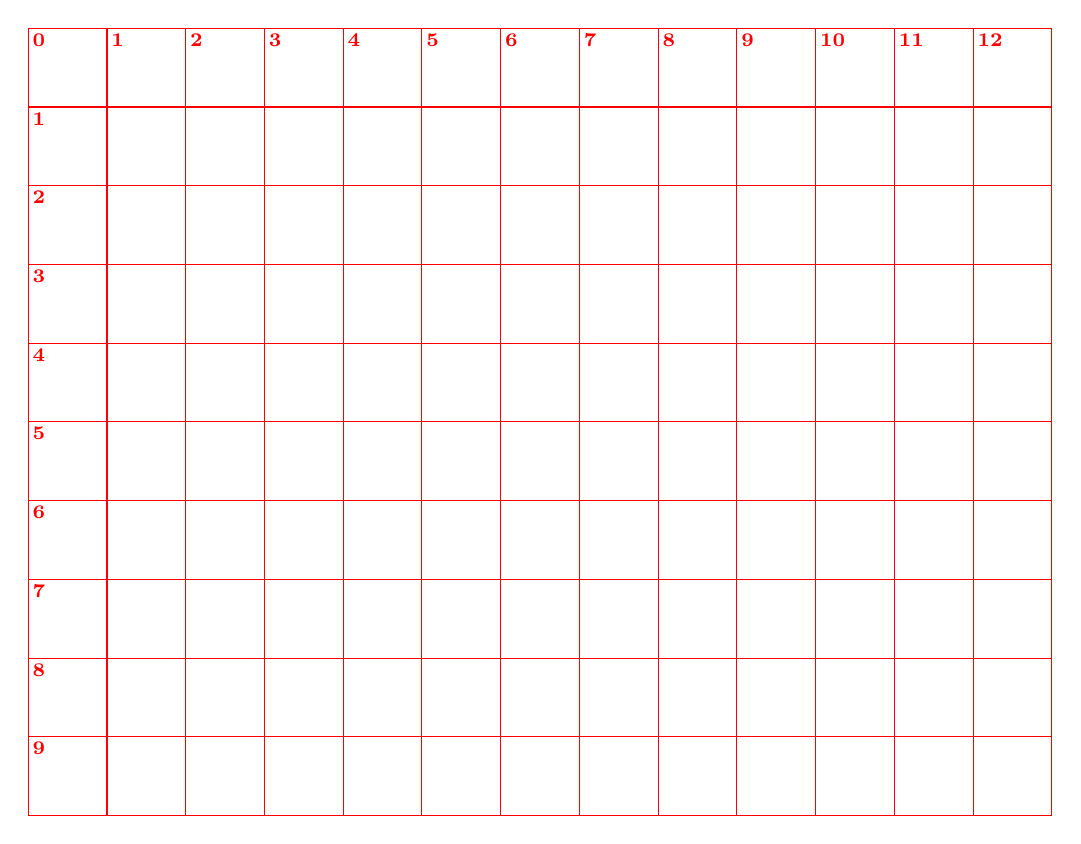
\begin{tikzpicture}[color=red]
      \draw[step=1cm] (0,0mm) grid (130mm,100mm);   
      \foreach \n in {0,...,12}
        \draw[xshift=.5mm,yshift=-1.5mm, inner sep=0pt, anchor=west] (\n,10) node {\scriptsize{\textbf{\n}}};
      \foreach \n in {1,...,9}
        \draw[xshift=.5mm,yshift=-1.5mm, inner sep=0pt, anchor=west] (0,10-\n) node {\scriptsize{\textbf{\n}}};
    \end{tikzpicture}
    \end{textblock*}
  }


%**
% \NormalBox<overlay spec>[tikz picture/node options]{<content>}
%
% draws content boxed in a nice box
% 
\newcommand<>{\NormalBox}[2][]{%
  \uncover#3{\tikz[#1, every node/.style={shape=rectangle, opacity=0.8, fill=white, drop shadow, inner sep=2pt, #1}]\node []{#2};}
}
%**
% \NormalBox<overlay spec>[tikz picture/node options]{<content>}
%
% draws content boxed in a nice box
% 
\newcommand<>{\RightArrow}[2][]{%
  \only#3{\tikz[#1, every node/.style={single arrow,draw=FireBrick,top color=OrangeRed!30, bottom color=Red!70!black, drop shadow, #1}]\node (ra) []{#2};}
}
\newcommand<>{\DownArrow}[2][]{%
  \only#3{\tikz[#1, every node/.style={single arrow,draw=FireBrick,right color=OrangeRed!30, left color=Red!70!black, drop shadow, shape border rotate=270, #1}]\node (da) []{#2};}
}
\newcommand<>{\FlashyBox}[2][]{%
  \only#3{\tikz[#1, every node/.style={rectangle,draw=FireBrick,right color=OrangeRed!30, left color=Red!70!black, drop shadow, shape border rotate=270, #1}]\node (fb) []{#2};}
}
%**
% \OrangeBox<overlay spec>[tikz picture/node options]{<content>}
%
% draws content boxed in an orange call-out box
% 
\newcommand<>{\OrangeBox}[2][]{%
  \onslide#3{\NormalBox[fill=orange!30,draw=black!30,rounded corners=4pt,#1]{#2}}%
} 



 % Keys to support piece-wise uncovering of elements in TikZ pictures:
  % \node[visible on=<2->](foo){Foo}
  % \node[visible on=<{2,4}>](bar){Bar}   % put braces around comma expressions
  %
  % Internally works by setting opacity=0 when invisible, which has the 
  % adavantage (compared to \node<2->(foo){Foo} that the node is always there, hence
  % always consumes space that (foo) is always available.
  %
  % The actual command that implements the invisibility can be overriden
  % by altering the style invisible. For instance \tikzsset{invisible/.style={opacity=0.2}}
  % would dim the "invisible" parts. Alternatively, the color might be set to white, if the
  % output driver does not support transparencies (e.g., PS) 
  %
  \tikzset{
    invisible/.style={opacity=0},
    visible on/.style={alt={#1{}{invisible}}},
    alt/.code args={<#1>#2#3}{%
      \alt<#1>{\pgfkeysalso{#2}}{\pgfkeysalso{#3}} % \pgfkeysalso doesn't change the path
    },
  }
  
  
%  \newcommand<>{\NormalBox}[2][]{%
%    \only#3{\tikz[#1, every node/.style={shape=rectangle,draw,fill=white, drop shadow, #1}]\node []{#2};}
%  }
  

% \setbeamertemplate{footline}[frame number]

\tikzfading[name=arrowfading, top color=transparent!0, bottom color=transparent!95]

\tikzset{arrowfillr/.style={top color=OrangeRed!20, bottom color=Red, general shadow={fill=black, shadow yshift=-0.8ex, path fading=arrowfading}}}
\tikzset{arrowstyler/.style 2 args={draw=FireBrick,arrowfillr, single arrow,minimum height=#1, minimum width=#2, single arrow,
single arrow head extend=.4cm,inner sep=1.5pt,}}


\tikzset{arrowfillb/.style={top color=PaleTurquoise, bottom color=DeepSkyBlue, general shadow={fill=black, shadow yshift=-0.8ex, path fading=arrowfading}}}
\tikzset{arrowstyleb/.style 2 args={draw=DarkBlue,arrowfillb, single arrow,minimum height=#1, minimum width=#2, single arrow,
single arrow head extend=.4cm,inner sep=1.5pt,}}

% \newcommand{\tikzfancyarrow}[2][2cm]{\tikz[baseline=-0.5ex]\node [arrowstyle=#1] {#2};}

\newcommand{\tikzfancyarrowr}[2][2cm]{\tikz[baseline=-0.5ex]\node [arrowstyler=#1] {#2};}
\newcommand{\tikzfancyarrowb}[2][2cm]{\tikz[baseline=-0.5ex]\node [arrowstyleb=#1] {#2};}


\input{sched_macros}
\input{theta_macros}
%
% \usetikzlibrary{external}
% \tikzexternalize
%

% \begin{filecontents}{\jobname.bib}
% \input{src/biblio/index.bib}
% \end{filecontents}
\usepackage[style=authoryear]{biblatex}
\renewcommand*{\nameyeardelim}{\addcomma\addspace}


\newcommand\grayed[1]{\textcolor{black!30}{#1}}

% \usepackage[normalem]{ulem}
% \usepackage{calc}
% \newsavebox\CBox
% \newcommand\hcancel[2][0.5pt]{%
%   \ifmmode\sbox\CBox{$#2$}\else\sbox\CBox{#2}\fi%
%   \makebox[0pt][l]{\usebox\CBox}%
%   \rule[0.5\ht\CBox-#1/2]{\wd\CBox}{#1}}
\usepackage{cancel}	

\usepackage{array}
\newcolumntype{L}[1]{>{\raggedright\let\newline\\\arraybackslash\hspace{0pt}}m{#1}}
\newcolumntype{C}[1]{>{\centering\let\newline\\\arraybackslash\hspace{0pt}}m{#1}}
\newcolumntype{R}[1]{>{\raggedleft\let\newline\\\arraybackslash\hspace{0pt}}m{#1}}


\usepackage{xspace}

\newcommand\pa[1]{\ensuremath{\left(#1\right)}}


\definecolor{cadmiumgreen}{rgb}{0.0, 0.42, 0.24}
\newcommand\mycitation[1]{{\scriptsize \textcolor{cadmiumgreen}{[#1]}}}
\newcommand\mycite[1]{{\scriptsize \textcolor{cadmiumgreen}{\parencite{#1}}}}

% \usepackage{tkz-graph}
% \usetikzlibrary{arrows,%
%                 petri,%
%                 topaths,%
% 								calc,%
% 								automata,
% 								positioning}%


\author{Emmanuel Hebrard}
\title{Resource Constraints in Scheduling}



%\addbibresource{\jobname.bib}
\addbibresource{src/biblio/index.bib}
\begin{document}


\maketitle



\section{Introduction}


	
\begin{frame}
	\frametitle{Content: constraint programming for scheduling}
	
	\pause
	\begin{myblock}{Part I: Propagation of resource constraints}
		\begin{itemize}
			\item Main bibliographic sources
			\begin{itemize}
				\item Constraint-based Scheduling~\mycite{BaptisteEtAl01}
				\item Petr Vil\'im's thesis~\mycite{VilimPhD}
			\end{itemize}
			\item Contributions of constraint programming to scheduling
			% \item The field of scheduling is {\it much} richer
		\end{itemize}
	\end{myblock}
	
	\pause
	\begin{myblock}{Part II: A very quick word on search}
		\begin{itemize}
			\item My biased view
		\end{itemize}
	\end{myblock}
	
	\pause
	\begin{myblock}{Part III: A glimpse of other types of resources}
		\begin{itemize}
			\item Resources come in every form and shape, Rosetta/Philae example
		\end{itemize}
	\end{myblock}
	
\end{frame}




\input{src/sections/examples.tex}

\begin{frame}
	
	\frametitle{Notations}
	
	\begin{center}
	\begin{itemize}
		\item A {\it task} $i$ is represented as a rectangle
		\begin{itemize}
			\item width represents \memph{processing time} $\dur{i}$ (possibly variable)
			\uncover<5->{
			\item height represents \memph{consumption} $\demand{i}$ (possibly variable)
			}
			\uncover<3->{
			\item its {\it domain} is given by its \memph{release date} $\est{i}$ and \memph{due date} $\lct{i}$
			\begin{itemize}
				\item we denote $\lst{i} = \lct{i}-\dur{i}$ its \memph{latest start time} and $\ect{i} = \est{i}+\dur{i}$ its \memph{earliest completion time}
			\end{itemize}
			}
		\end{itemize}
		\uncover<2->{
		\item There can be {\it precedences} between start or end of tasks
		}
		\uncover<4->{
		\item There can be {\it resources} required by some tasks\uncover<5->{, with a given \memph{capacity} $\capacity$}
		}
	\end{itemize}
	
	\medskip
	\medskip

	\begin{colorschedfigure}{.45}
	\input{ex/notation.tex}

	\uncover<3>{
	\draw[thick, densely dashed, color=bostonuniversityred] (0,-5) -- (0, -6.7);
	\node[] at (0, -7) {\scriptsize $\est{{\rm Civa}}$};
	\draw[thick, densely dashed, color=bostonuniversityred] (18,-5) -- (18, -6.7);
	\node[] at (18, -7) {\scriptsize $\lct{{\rm Civa}}$};
	
	\PhantomExtensibleTask{12}{6}{6}{1}{5}{}{Civa}
	
	\draw[thick, densely dashed, color=bostonuniversityred] (6,-5) -- (6, -6.7);
	\node[] at (6, -7) {\scriptsize $\ect{{\rm Civa}}$};
	\draw[thick, densely dashed, color=bostonuniversityred] (12,-5) -- (12, -6.7);
	\node[] at (12, -7) {\scriptsize $\lst{{\rm Civa}}$};
	}
	\end{colorschedfigure}
	\end{center}

\end{frame}


\begin{frame}
\frametitle{Scheduling problem}

\begin{itemize}
	\item Assign a {start time} \memph{$\stof{i}$} and an {completion time} \memph{$\ctof{i}$} to every task \memph{$i \in {\cal T}$} such that:
	\begin{itemize}
		\item Precedence constraints are satisfied
		\item Resource constraints are satisfied
	\end{itemize}
	
	\pause
	\item Objectives:
	\begin{itemize}
		\item Minimize {makespan} (\memph{$\max\{\lct{i} \mid i \in {\cal T}\}$})
		% \item Minimize total tardiness ($\sum_{i \in {\cal T}} \max(0, \lst{i}-)$)
		\item Minimize total weighted tardiness (\memph{$\sum_{i \in {\cal T}} w_i \max(0, \lct{i}-\delta_i)$})
		\item ...
	\end{itemize}
	
	\pause
	\item Within Constraint Programming: not so important
	\begin{itemize}
		\item Handled by a constraint
		\item Depend on start and end times of tasks
	\end{itemize}
	
\end{itemize}

	
\end{frame}




\begin{frame}
	\frametitle{Constraint vs Algorithm}
	
	\begin{itemize}
		\item Constraints \& models written using {\it variables} symbols (\memph{\stof{i}, \ctof{i}})
		\item Algorithmic rules written using {\it domain} symbols (\memph{\est{i},\lst{i},\ect{i},\lct{i}})
		% \begin{itemize}
		% 	\item In some references ``data'' {\it release/due dates} might be differentiated from ``variables'' {\it earliest start/latest completion times} (not here)
		% \end{itemize}
		\uncover<2-> {
		\item Example: precedence \memph{$i \prec j$}
		\uncover<2-> {
		\begin{itemize}
			\item Constraint predicate:\begin{eqnarray*}
				\memph{\ctof{i} \leq \stof{j}}
			\end{eqnarray*}
			\uncover<3-> {
			\item Algorithmic rules:\begin{eqnarray*}
				\memph{\ect{i} > \est{j} \implies \est{j} = \ect{i}} \\
				\memph{\lst{j} < \lct{i} \implies \lct{i} = \lst{j}} 
			\end{eqnarray*}
			}
		\end{itemize}
		}
		}
		\uncover<4-> {
		\item Notion of \memph{consistency}: constraints are sufficient to define the \memph{result} of propagation
		}
	\end{itemize}
	
	% si:[0,2] ei:[4,6]
	% sj:[4,6] ej:[8,10]
	
	% \forall t & \memph{\ect{i} \geq t \implies \est{j} \geq t} \\
	% & \memph{\lst{j} \leq t \implies \lct{i} \leq t}
	
\end{frame}


\begin{frame}
	\frametitle{Bound consistency}
	
	\begin{columns}
	
	\column{.56\textwidth}
	\begin{myblock}{Constraint \memph{$C$} over variables \memph{${\cal X}$}}
			\begin{itemize}
				\item \memph{$C$}: predicate defining a relation in \memph{$\mathbb{N}^{|{\cal X}|}$}
			\end{itemize}
	\end{myblock}
	
	\uncover<2->{
	\begin{myblock}{Bound support \memph{$\sigma$} of \memph{$x,t$} for $C$ over ${\cal X}$}
			\begin{itemize}
				\item $\sigma: {\cal X} \mapsto \mathbb{N}$ with $\sigma(x)=t$
				\item \memph{valid} $\iff \forall x \in {\cal X}~ \min(x) \leq \sigma(x) \leq \max(x)$ 
				\item \memph{consistent} $\iff C(\sigma({\cal X}))$ 
			\end{itemize}
	\end{myblock}
	}
	
	\column{.02\textwidth}
	
	\column{.42\textwidth}

	Ex: $i \prec j$
	\begin{itemize}
		\item Predicate: \memph{$\ctof{i} \leq \stof{j}$}
		
		\begin{colorschedfigure}{.4}
			\PrintTics{0,5,...,11}{1}
			\PrintGrid{10}{2}
			\uncover<1-2>{
			\ExtensibleVariableTask{0.000000}{10.000000}{4.000000}{4.000000}{1}{0}{A}{$i$}
			\ExtensibleVariableTask{0.000000}{10.000000}{4.000000}{4.000000}{1}{1}{A}{$j$}
			}
			\uncover<3->{
			\ExtensibleVariableTask{0.000000}{6.000000}{4.000000}{4.000000}{1}{0}{A}{$i$}
			\ExtensibleVariableTask{4.000000}{10.000000}{4.000000}{4.000000}{1}{1}{A}{$j$}
			\PrunedExtensibleTask{0.000000}{4.000000}{4.000000}{1}{1}{A}{}
			\PrunedExtensibleTask{6.000000}{4.000000}{4.000000}{1}{0}{A}{}
			}
		\end{colorschedfigure}
		
		\uncover<2->{
		\item Ex.: no valid and consistent bound support for $\ctof{i} = 7$
		\begin{itemize}
			\item consistent: $\langle \ctof{i}:7, \stof{j}:7 \rangle$
			\item valid: $\langle \ctof{i}:7, \stof{j}:6 \rangle$
		\end{itemize}
		}
		
	\end{itemize}

	\end{columns}
	
	\uncover<3->{
	\begin{itemize}
		\item Result of propagation algorithm is entailed by ``{\it bound consistency on $\ctof{i} \leq \stof{j}$}''
		\item Its complexity is not
	\end{itemize}
	}
	
\end{frame}


\begin{frame}
	\frametitle{Resource Constraint}
	
	\begin{itemize}
		\item Very rich taxonomy of resources
		\item Focus on Renewable, discrete, non-interruptible, cumulative resource
	\end{itemize}
	
	\begin{myblock}{A model of {\sc CumulativeResource}}
		\begin{itemize}
			\item \memph{Processing time}: require the resources for at least $\dur{i}$ time \hfill $\stof{i} + \dur{i} \geq \ctof{i}~\forall i$
			\item \memph{Non preemption}: cannot be interrupted \hfill $\stof{i} + \dur{i} \leq \ctof{i}~\forall i$
			\item \memph{Bounds}: release and due dates  \hfill  $\est{i} \leq \stof{i} \leq \ctof{i} \leq \lct{i}~\forall i$
			\item \memph{Resource capacity}: additive, upper bounded resource usage \hfill $\sum_{\stof{i} \leq t \leq \ctof{i}} \demand{i} \leq \capacity~\forall t$
		\end{itemize}
	\end{myblock}
	
	\uncover<2-> {
	\begin{itemize}
		\item {\bf File transfer}; memory bank: \memph{Single-machine} resource (\memph{$\demand{i}=\capacity=1$})
		\uncover<3-> {
		\item {\bf File transfer}; download channel: \memph{m-machine} resource (\memph{$\demand{i}=1, \capacity>1$})
		}
		\uncover<4-> {
		\item {\bf Philae}; battery power threshold: \memph{cumulative} resource (\memph{$\demand{i} \geq 1, \capacity>1$})
		}
	\end{itemize}
	}
	
\end{frame}



\begin{frame}
	\frametitle{Coping with NP-hardness}

	\begin{columns}
		
		\column{.18\textwidth}
		
		\column{.64\textwidth}
		
	\begin{myblock}{A \only<1-2>{model}\only<3->{\memph{decomposition}} of {\sc CumulativeResource}}
		\vspace{-.5cm}
		\begin{eqnarray*}
			\stof{i} + \dur{i} \geq \ctof{i} & \forall i \\
			\stof{i} + \dur{i} \leq \ctof{i} & \forall i \\
			\est{i} \leq \stof{i} \leq \ctof{i} \leq \lct{i} & \forall i \\
			\sum_{\stof{i} \leq t \leq \ctof{i}} \demand{i} \leq \capacity & \forall t
		\end{eqnarray*}
	\end{myblock}
	
	\column{.18\textwidth}
	
	\end{columns}

	\begin{itemize}
		\item The problem {\sc CumulativeResource} is strongly NP-hard
		\begin{itemize}
			\item So is bound consistency, since a bound support is a valid schedule
		\end{itemize}
		\uncover<2->{
		\item \memph{Relaxation}: if the relaxed problem is unsatisfiable, so is the original problem
		\uncover<3->{
		\item \memph{Decomposition}: 
		\begin{itemize}
			\item Enforcing bound consistency on {\sc CumulativeResource} is NP-hard (global support)
			\item Enforcing bound consistency on the model above is polynomial (local supports)
		\end{itemize}
		}
		}
	\end{itemize}	
	
	

	
\end{frame}



% \subsection{Goals}


\section{Time-tabling}

\begin{frame}
\frametitle{Time-tabling}

\begin{itemize}
	\item Notion of ``compulsory part'' \mycite{Lahrichi82}
	\begin{itemize}
		\item Period in which the task must be in process
	\end{itemize}

	\uncover<4->{
	\item Notion of ``time-tables'' \mycite{LePapePhD}, ``resource profile'' \mycite{Fox90}, ``resource histogram'' \mycite{CaseauLaburthe96}
	\begin{itemize}
		\item Minimum usage of the resource over time
	\end{itemize}
	}
\end{itemize}

\begin{center}
	\begin{colorschedfigure}{.6}
		\begin{frame}
\frametitle{Time-tabling}

\begin{itemize}
	\item Notion of ``compulsory part'' \mycite{Lahrichi82}
	\begin{itemize}
		\item Period in which the task must be in process
	\end{itemize}

	\uncover<4->{
	\item Notion of ``time-tables'' \mycite{LePapePhD}, ``resource profile'' \mycite{Fox90}, ``resource histogram'' \mycite{CaseauLaburthe96}
	\begin{itemize}
		\item Minimum usage of the resource over time
	\end{itemize}
	}
\end{itemize}

\begin{center}
	\begin{colorschedfigure}{.6}
		\begin{frame}
\frametitle{Time-tabling}

\begin{itemize}
	\item Notion of ``compulsory part'' \mycite{Lahrichi82}
	\begin{itemize}
		\item Period in which the task must be in process
	\end{itemize}

	\uncover<4->{
	\item Notion of ``time-tables'' \mycite{LePapePhD}, ``resource profile'' \mycite{Fox90}, ``resource histogram'' \mycite{CaseauLaburthe96}
	\begin{itemize}
		\item Minimum usage of the resource over time
	\end{itemize}
	}
\end{itemize}

\begin{center}
	\begin{colorschedfigure}{.6}
		\input{ex/timetabling_intuition.tex}
	\end{colorschedfigure}
\end{center}

\end{frame}

% \begin{frame}
% \frametitle{Time-tabling}
%
% \begin{center}
% 	\begin{colorschedfigure}{.6}
% 		\input{ex/cumulative_timetabling.tex}
% 	\end{colorschedfigure}
% \end{center}
%
% \end{frame}


	\end{colorschedfigure}
\end{center}

\end{frame}

% \begin{frame}
% \frametitle{Time-tabling}
%
% \begin{center}
% 	\begin{colorschedfigure}{.6}
% 		\input{ex/cumulative_timetabling.tex}
% 	\end{colorschedfigure}
% \end{center}
%
% \end{frame}


	\end{colorschedfigure}
\end{center}

\end{frame}

% \begin{frame}
% \frametitle{Time-tabling}
%
% \begin{center}
% 	\begin{colorschedfigure}{.6}
% 		\input{ex/cumulative_timetabling.tex}
% 	\end{colorschedfigure}
% \end{center}
%
% \end{frame}



\begin{frame}
\frametitle{Time-tabling decomposition}

\begin{itemize}
	\item Boolean variables \memph{\patvar{i}{t}} standing for: ``task \memph{$i$} is in process at time \memph{$t$}''
	\item Enforce bounds consistency on:
\end{itemize}
\begin{eqnarray}
	%\forall i \in {\cal T}, \forall t \in [1,h] & \memph{\patvar{i}{t} \in \{0,1\}} \\
	\forall i  & {\stof{i} + \dur{i} = \ctof{i}} & {\hfill \scriptsize \textrm{processing~time~\&~non-preemption}} \\
	\forall t  & {\sum_{i \in {\cal T}} \demand{i}\patvar{i}{t} \leq \capacity} & {\hfill \scriptsize \textrm{resource~capacity}} \\
	\forall i \forall t & \memph{\patvar{i}{t} \iff \stof{i} \leq t \wedge t < \ctof{i}} & {\hfill \scriptsize \textrm{channeling}} 
	 % & \memph{(\neg\patvar{i}{t} \wedge t < \ect{i}) \implies \stof{i} > t} \\
	 % & \memph{(\neg\patvar{i}{t} \wedge t \geq \lst{i}) \implies \ctof{i} \leq t}
\end{eqnarray}\begin{center}
	\begin{colorschedfigure}{.45}
		\input{ex/unary_timetabling.tex}
	\end{colorschedfigure}\begin{scriptsize}
	\begin{tabular}{C{1.35cm}C{1.35cm}C{1.35cm}C{1.35cm}C{1.35cm}}
		\only<1-4>{$\{0,1\}$}\only<5->{$\{1\}$} &
		\only<1>{$\{0,1\}$}\only<2->{$\{1\}$} &
		\only<1-2>{$\{0,1\}$}\only<3->{$\{0\}$} &
		\only<1-2>{$\{0,1\}$}\only<3->{$\{0\}$} & ~\\

		\only<1-4>{$\{0,1\}$}\only<5->{$\{0\}$} &
		\only<1>{$\{0,1\}$}\only<2->{$\{0\}$} &
		\only<1-2>{$\{0,1\}$}\only<3->{$\{1\}$} &
		\only<1-2>{$\{0,1\}$}\only<3->{$\{1\}$} & ~
	\end{tabular}\end{scriptsize}\end{center}\uncover<2->{
\begin{itemize}
	\item $\memph{\stof{A} \leq 1 \wedge 1 < \ctof{A}} \Rightarrow \memph{\patvar{A}{1} = 1}$ \hfill $A$ must be in process at $t=1$
	\item $\Rightarrow \memph{\patvar{B}{1} = 0} \Rightarrow \memph{\ctof{B} \leq 1 \vee 1 < \stof{B}}$ \hfill $B$ cannot be in process at $t=1$
	\uncover<3->{
	\item $\Rightarrow \memph{1 < \stof{B}}$ \hfill $B$ cannot end earlier than $t=2$ so it must start at $t \geq 2$
	}
\end{itemize}
}

\end{frame}



% \begin{frame}
% \frametitle{Time-tabling decomposition}
%
% \begin{itemize}
% 	\item Straightforward generalisation to cumulative constraints
% \end{itemize}
%
% \begin{eqnarray}
% 	%\forall i \in {\cal T}, \forall t \in [1,h] & {\patvar{i}{t} \in \{0,1\}} \\
% 	\forall i & \stof{i} + \dur{i} = \ctof{i} & {\hfill \scriptsize \textrm{processing~time~\&~non-preemption}} \\
% 	\forall t & {\sum_{i \in {\cal T}} \memph{\demand{i}}\patvar{i}{t} \leq \memph{\capacity}} & {\hfill \scriptsize \textrm{resource~capacity}} \\
% 	\forall i \forall t & {\patvar{i}{t} \iff \stof{i} \leq t \wedge t < \ctof{i}} & {\hfill \scriptsize \textrm{channeling}}
% \end{eqnarray}
%
% \begin{center}
% 	\begin{colorschedfigure}{.45}
% 		\input{ex/cumulative_timetabling.tex}
% 	\end{colorschedfigure}
% \end{center}
%
% \end{frame}







\begin{frame}
\frametitle{Time-tabling algorithm: satisfiability check}

\begin{columns}
	\column{.35\textwidth}

	\begin{myblock}{Resource profile}
		\uncover<2->{
		\begin{itemize}
			\item Compute compulsory parts
			\uncover<3->{
			\item Sort ``events'' (start and end times of compulsory parts) ($O(n \log n)$)
			}
			\uncover<4->{
			\item Process events to compute the profile \memph{$P$} ($O(n)$)
			}
			\uncover<5->{
			\item \memph{Sweep} algorithm \mycite{BeldiceanuCarlsson01} (more general)
			}
		\end{itemize}
		}
	\end{myblock}

	\column{.65\textwidth}
	\begin{colorschedfigure}{.28}
		\input{ex/timetabling_profile.tex}
				\uncover<3>{
					\draw[color=bostonuniversityred, densely dotted, thick] (4,-6) -- (4,-17.8);
					\node[color=bostonuniversityred] at (4,-18.5) {\tiny +4};
					\draw[color=bostonuniversityred, densely dotted, thick] (7,-6) -- (7,-18.8);
					\node[color=bostonuniversityred] at (7,-19.5) {\tiny -4};

					\draw[color=bostonuniversityred, densely dotted, thick] (9,-10) -- (9,-17.8);
					\node[color=bostonuniversityred] at (8.8,-18.5) {\tiny +4};
					\draw[color=bostonuniversityred, densely dotted, thick] (12,-4) -- (12,-17.8);
					\node[color=bostonuniversityred] at (12,-18.5) {\tiny +3};
					\node[color=bostonuniversityred] at (12,-19.5) {\tiny -4,-2};
					\draw[color=bostonuniversityred, densely dotted, thick] (10,-4) -- (10,-17.8);
					\node[color=bostonuniversityred] at (10.2,-18.5) {\tiny +2};
					\draw[color=bostonuniversityred, densely dotted, thick] (15,-14) -- (15,-18.8);
					\node[color=bostonuniversityred] at (15,-19.5) {\tiny -4};

					\draw[color=bostonuniversityred, densely dotted, thick] (16,0) -- (16,-17.8);
					\node[color=bostonuniversityred] at (16,-18.5) {\tiny +4};
					\draw[color=bostonuniversityred, densely dotted, thick] (17,0) -- (17,-18.8);
					\node[color=bostonuniversityred] at (17,-19.5) {\tiny -4};

				}
	\end{colorschedfigure}
\end{columns}

\end{frame}


\begin{frame}
\frametitle{Time-tabling algorithm: bound propagator}

	\begin{itemize}
		\item Assume \memph{$\capacity=3$} and consider the profile interval \memph{$[5,10):2$}
		\uncover<2->{
		\item A task \only<2-3>{\memph{$A$} such that $[\est{A},\lst{A})$ overlaps with $[5,10)$}\only<4->{\memph{$B$} counted in the profile}
		}
		\uncover<6->{
		\item $[a,b)$ overlaps with $[\est{i},\min(\lst{i},\ect{i})) \implies \est{i} = \min(b,\lst{i})$  
		}
	\end{itemize}

\begin{center}
\begin{colorschedfigure}{.5}

\PrintTics{0,3,...,15}{1.000000}
\PrintGrid{15}{2}
% \MandatoryPartTask{0.000000}{5.000000}{15.000000}{2}{0}{A}{A}

\CProfile{{0.000000/0/5.000000/2, 5.000000/2/10.000000/0, 10.000000/0/15.000000/0}}{2}{4.700000}{A}{15.000000}

\uncover<2>{
\LeftExtensibleVariableTask{3}{15}{5}{5}{2}{0}{A}{A}
\draw[color=bostonuniversityred, very thick, dotted] (3,0) -- (3,-3);
\draw[color=bostonuniversityred, very thick, dotted] (8,0) -- (8,-3);
}
\uncover<3>{
\GroundTask{10}{5}{2}{0}{A}{A}
\PrunedExtensibleTask{3}{7}{7}{2}{0}{A}{}
}

\uncover<4-5>{
\MandatoryPartTask{2.000000}{3.000000}{13.000000}{2}{0}{A}{B}
\draw[color=bostonuniversityred, very thick, dotted] (2,0) -- (2,-3);
\uncover<4>{
\draw[color=bostonuniversityred, very thick, dotted] (10,0) -- (10,-3);
}
\uncover<5>{
\draw[color=bostonuniversityred, very thick, dotted] (7,0) -- (7,-3);
}
}
\uncover<6->{
\GroundTask{7}{8}{2}{0}{A}{B}
\PrunedExtensibleTask{2}{5}{5}{2}{0}{A}{}
}


\end{colorschedfigure}
\end{center}

\end{frame}


\begin{frame}
\frametitle{Time-tabling algorithm: bound propagator}

\begin{columns}
	\column{.35\textwidth}


	\begin{itemize}
		\item Interval \memph{$[a,b):h$}, Task \memph{$i$}
		\begin{itemize}
			\item \memph{overloaded} iff \memph{$\demand{i}+h > \capacity$}
			\item \memph{relevant} iff
				\begin{itemize}
					\item \memph{$\est{i} < b$} and
					\item \memph{$\min(\ect{i},\lst{i}) > a$}
				\end{itemize}
			% \item \memph{forbidden} iff \memph{$\min(\ect{i},\lst{i}) > a$}
		\end{itemize}
		%
		% \item Adjust \memph{$\est{i}$} to \memph{$b$} if \memph{$\exists [a,b) \in P$} of height \memph{$h$} such that:
		% \begin{itemize}
		% 	\item \memph{$\demand{i}+h > \capacity$} {\scriptsize (overload)}
		% 	\item \memph{$\min(\ect{i}, \lst{i}) > a$} {\scriptsize (is not counted in, and cannot end before, the peak)}
		% \end{itemize}
	\end{itemize}

	\uncover<2->{
	\begin{myblock}{Algorithm \mycite{OuelletQuimper13}}
	\begin{itemize}
		\item {\scriptsize compute profile}
		\uncover<3->{
		\item {\scriptsize order chuncks by decreasing \memph{$h$}}
		\item {\scriptsize for \memph{$i \in {\cal T}$} by increasing \memph{$\demand{i}$}:}
		\begin{itemize}
			\item {\scriptsize add \memph{$i$}'s over. intervals to \memph{$S$}}
			\uncover<4->{
			\item {\scriptsize get \memph{$i$}'s relevant interval in \memph{$S$}}
			\begin{itemize}
				\item $O(\log n)$ if \memph{$S$} is an AVL tree
			\end{itemize}
			}
		\end{itemize}
		}
	\end{itemize}
	\end{myblock}
	}
	\column{.65\textwidth}
	\begin{colorschedfigure}{.28}
		\input{ex/timetabling.tex}
		\uncover<3-5>{
		\draw[color=bostonuniversityred, ultra thick] (10,-17.5) -- (12,-17.5);
		}
		\uncover<4-5>{
			\node[color=bostonuniversityred] at (10,-18) {\tiny $a$};
			\node[color=bostonuniversityred] at (12,-18) {\tiny $b$};
		}
		\uncover<4>{
		\node[color=bostonuniversityred] at (5,-3.5) {\tiny $\est{E}$};
		\node[color=bostonuniversityred] at (11,-3.5) {\tiny $\min(\ect{E},\lst{E})$};
			\draw[color=bostonuniversityred, very thick, dotted] (5,-4) -- (5,-17.5);
			\draw[color=bostonuniversityred, very thick, dotted] (10,-4) -- (10,-17.5);
		}
		\uncover<5>{
		\node[color=bostonuniversityred] at (7,-13.5) {\tiny $\est{D}$};
		\node[color=bostonuniversityred] at (13,-13.5) {\tiny $\min(\ect{C},\lst{D})$};
			\draw[color=bostonuniversityred, very thick, dotted] (7,-14) -- (7,-17.5);
			\draw[color=bostonuniversityred, very thick, dotted] (12,-14) -- (12,-17.5);
		}

		\uncover<6>{
			\node[color=bostonuniversityred] at (4,-18) {\tiny $a$};
			\node[color=bostonuniversityred] at (7,-18) {\tiny $b$};
			\draw[color=bostonuniversityred, ultra thick] (9,-17.5) -- (12,-17.5);
			\draw[color=bostonuniversityred, ultra thick] (4,-17.5) -- (7,-17.5);
			\node[color=bostonuniversityred] at (6,-9.5) {\tiny $\est{C}$};
			\node[color=bostonuniversityred] at (10,-9.5) {\tiny $\min(\ect{C},\lst{C})$};
			\draw[color=bostonuniversityred, very thick, dotted] (6,-10) -- (6,-17.5);
			\draw[color=bostonuniversityred, very thick, dotted] (9,-10) -- (9,-17.5);
		}
	\end{colorschedfigure}
\end{columns}

\end{frame}

\begin{frame}
    \frametitle{Time-tabling Algorithms}

		\begin{itemize}
			\item Sweep algorithm \mycite{BeldiceanuCarlsson01}
			\item $O(n^2)$ synchornized sweep algoritm \mycite{LetortEtAl12}
			\item $O(n \log n)$ algorithm \mycite{OuelletQuimper13}
			\item $O(n)$ algorithm (not pracical) and  $O(n^2)$ efficient and simple algorithm \mycite{GayEtAl15}
		\end{itemize}

\end{frame}


\begin{frame}
    \frametitle{PySched -- Available on GitHub}
		\includegraphics[width=\textwidth]{im/code.png}
\end{frame}






\section{Disjunctive reasoning}

\begin{frame}
\frametitle{Disjunctive constraints}

\begin{itemize}
	\item Change the viewpoint (variables) from start times to precedences
	\item Notion of disjunctive graph \mycite{RoySussman64} central to \mycite{CarlierPinson89}'s method
	\begin{itemize}
		\item If \memph{$i$} and \memph{$j$} require the same exclusive resource\uncover<2->{, then either \memph{$i \prec j$} \uncover<3->{or \memph{$j \prec i$}}}
	\end{itemize}
\end{itemize}

\begin{center}
	\begin{colorschedfigure}{.45}
		\input{ex/disjunctive_example.tex}
	\end{colorschedfigure}
\end{center}

\end{frame}


\begin{frame}
\frametitle{Disjunctive decomposition (single-machine)}

\begin{eqnarray*}
	\forall i<j \in {\cal T}, &  \memph{\precvar{i}{j} \iff \ctof{i} \leq \stof{j}} \\
	 &  \memph{\precvar{i}{j} \neq \precvar{j}{i}}
\end{eqnarray*}

\begin{center}
	\begin{colorschedfigure}{.45}
		\begin{frame}
\frametitle{Disjunctive constraints}

\begin{itemize}
	\item Change the viewpoint (variables) from start times to precedences
	\item Notion of disjunctive graph \mycite{RoySussman64} central to \mycite{CarlierPinson89}'s method
	\begin{itemize}
		\item If \memph{$i$} and \memph{$j$} require the same exclusive resource\uncover<2->{, then either \memph{$i \prec j$} \uncover<3->{or \memph{$j \prec i$}}}
	\end{itemize}
\end{itemize}

\begin{center}
	\begin{colorschedfigure}{.45}
		\input{ex/disjunctive_example.tex}
	\end{colorschedfigure}
\end{center}

\end{frame}


\begin{frame}
\frametitle{Disjunctive decomposition (single-machine)}

\begin{eqnarray*}
	\forall i<j \in {\cal T}, &  \memph{\precvar{i}{j} \iff \ctof{i} \leq \stof{j}} \\
	 &  \memph{\precvar{i}{j} \neq \precvar{j}{i}}
\end{eqnarray*}

\begin{center}
	\begin{colorschedfigure}{.45}
		\begin{frame}
\frametitle{Disjunctive constraints}

\begin{itemize}
	\item Change the viewpoint (variables) from start times to precedences
	\item Notion of disjunctive graph \mycite{RoySussman64} central to \mycite{CarlierPinson89}'s method
	\begin{itemize}
		\item If \memph{$i$} and \memph{$j$} require the same exclusive resource\uncover<2->{, then either \memph{$i \prec j$} \uncover<3->{or \memph{$j \prec i$}}}
	\end{itemize}
\end{itemize}

\begin{center}
	\begin{colorschedfigure}{.45}
		\input{ex/disjunctive_example.tex}
	\end{colorschedfigure}
\end{center}

\end{frame}


\begin{frame}
\frametitle{Disjunctive decomposition (single-machine)}

\begin{eqnarray*}
	\forall i<j \in {\cal T}, &  \memph{\precvar{i}{j} \iff \ctof{i} \leq \stof{j}} \\
	 &  \memph{\precvar{i}{j} \neq \precvar{j}{i}}
\end{eqnarray*}

\begin{center}
	\begin{colorschedfigure}{.45}
		\input{ex/disjunctive.tex}
	\end{colorschedfigure}
\end{center}

\uncover<4->{
\begin{itemize}
	\item \memph{Completeness} of disjunctive propagation: deciding only \memph{$\precvar{i}{j}$} variables is sufficient
\end{itemize}
}

% \begin{myblock}{Restricting}
% 	\begin{itemize}
% 		\item Implication is trivial, equivalence might not be
% 		\begin{itemize}
% 			\item
% 		\end{itemize}
% 	\end{itemize}
% \end{myblock}

\end{frame}

\newcommand\istrue[1]{[{#1}]}
\newcommand\isfalse[1]{\neg [{#1}]}

\begin{frame}
\frametitle{Disjunctive algorithm}

\begin{eqnarray*}
	\forall i<j \in {\cal T}, &  {\istrue{\precvar{i}{j}} \implies {i} \prec {j}} & {\footnotesize \hfill \textrm{(post~}{i} \prec {j}\textrm{'s~propagator)}} \\
														&  \only<1-4>{\isfalse{\precvar{i}{j}} \implies {j} \prec {i}}\only<5->{\memph{\isfalse{\precvar{i}{j}} \implies {j} \prec {i}}} & {\footnotesize \hfill \textrm{(post~}{j} \prec {i}\textrm{'s~propagator)}}\\
														& {\ect{j} > \lst{i} \implies \istrue{\precvar{i}{j}}} \\
														& \only<1-3>{\ect{i} > \lst{j} \implies \isfalse{\precvar{i}{j}}}\only<4->{\memph{\ect{i} > \lst{j} \implies \isfalse{\precvar{i}{j}}}}
\end{eqnarray*}


\begin{columns}
	
	\column{.6\textwidth}

\uncover<2->{
\begin{myblock}{Strictly stronger than Time-tabling}
	\begin{itemize}
		\item Suppose $\patvar{i}{t} = 0$ and $\ctof{i} > t$
		\uncover<3->{
		\begin{itemize}
			\item $\exists j$ s.t. $\patvar{j}{t} = 1$ \uncover<4->{hence \memph{$\lst{j} \leq t < \ect{j}$}}
			\uncover<4->{
			\item Therefore, \memph{$\lst{j} < \ect{i}$} so \memph{$\precvar{i}{j}$} must be false
			\uncover<5->{
			\item and thus \memph{${j} \prec {i}$} is posted
			}			
			}
		\end{itemize}
		}
	\end{itemize}
\end{myblock}
}

	\column{.4\textwidth}

\uncover<2->{
		\begin{colorschedfigure}{.4}
			\PrintTics{0,10,...,11}{1}
			\PrintGrid{10}{2}
			\uncover<1->{
			\LeftExtensibleVariableTask{2.000000}{10.000000}{5.000000}{5.000000}{1}{0}{A}{$i$}
			}
			\uncover<2->{
			\ExtensibleTask{5}{1}{1}{1}{0}{E}{}	
			\node[] at (5.5, .5) {$t$};
			
			\uncover<3->{
			\MandatoryPartTask{3.000000}{1.000000}{5.000000}{1}{1}{A}{$j$}
			}
			
			\uncover<4->{
			\draw[thick, densely dashed, color=bostonuniversityred] (7,0) -- (7, -2.3);
			\node[] at (7, -3) {\scriptsize $\ect{i}$};
			
			\draw[thick, densely dashed, color=bostonuniversityred] (5,-1) -- (5, -3.3);
			\node[] at (5, -4) {\scriptsize $\lst{j}$};
			}
			
			% \ExtensibleVariableTask{0.000000}{10.000000}{4.000000}{4.000000}{1}{1}{A}{$j$}
			}
			% \uncover<2>{
			% \ExtensibleVariableTask{0.000000}{6.000000}{4.000000}{4.000000}{1}{0}{A}{$i$}
			% \ExtensibleVariableTask{4.000000}{10.000000}{4.000000}{4.000000}{1}{1}{A}{$j$}
			% \PrunedExtensibleTask{0.000000}{4.000000}{4.000000}{1}{1}{A}{}
			% \PrunedExtensibleTask{6.000000}{4.000000}{4.000000}{1}{0}{A}{}
			% }
		\end{colorschedfigure}	
	}
	
\end{columns}

\end{frame}
\begin{frame}
\frametitle{Generalisation to cumulative resources}

\begin{itemize}
	\item Either \memph{$i \prec j$}, \memph{$j \prec i$} or \memph{$i \not\prec j \wedge j \not\prec i$}
	\begin{itemize}
		\item Easy change: \memph{$\precvar{i}{i} \neq \precvar{j}{i}$} becomes \memph{$\neg(\precvar{i}{j} \wedge \precvar{j}{i})$}, but not complete anymore! 
	\end{itemize}
	
	% \uncover<2->{
	% \item Straightforward ``particular case'' generalisation \mycite{BaptisteEtAl01}
	% \begin{itemize}
	% 	\item \memph{$\demand{i}+\demand{j}>\capacity \implies \precvar{i}{j} \vee \precvar{j}{i}$}
	% \end{itemize}
	\uncover<2->{
	\item To keep the property that start times do not need to be set:
	
	\begin{itemize}
	\item For every \memph{minimal} subset \memph{$S$} of tasks such that \memph{$\sum_{i \in S}\demand{i} > \capacity$}, post:
	% \begin{itemize}
		% \item
		\memph{$$\bigvee_{i \neq j \in S} \precvar{i}{j}$$}
	% \end{itemize}
	\item Not used in practice
	\end{itemize}
	}
	% }
\end{itemize}

\end{frame}




	\end{colorschedfigure}
\end{center}

\uncover<4->{
\begin{itemize}
	\item \memph{Completeness} of disjunctive propagation: deciding only \memph{$\precvar{i}{j}$} variables is sufficient
\end{itemize}
}

% \begin{myblock}{Restricting}
% 	\begin{itemize}
% 		\item Implication is trivial, equivalence might not be
% 		\begin{itemize}
% 			\item
% 		\end{itemize}
% 	\end{itemize}
% \end{myblock}

\end{frame}

\newcommand\istrue[1]{[{#1}]}
\newcommand\isfalse[1]{\neg [{#1}]}

\begin{frame}
\frametitle{Disjunctive algorithm}

\begin{eqnarray*}
	\forall i<j \in {\cal T}, &  {\istrue{\precvar{i}{j}} \implies {i} \prec {j}} & {\footnotesize \hfill \textrm{(post~}{i} \prec {j}\textrm{'s~propagator)}} \\
														&  \only<1-4>{\isfalse{\precvar{i}{j}} \implies {j} \prec {i}}\only<5->{\memph{\isfalse{\precvar{i}{j}} \implies {j} \prec {i}}} & {\footnotesize \hfill \textrm{(post~}{j} \prec {i}\textrm{'s~propagator)}}\\
														& {\ect{j} > \lst{i} \implies \istrue{\precvar{i}{j}}} \\
														& \only<1-3>{\ect{i} > \lst{j} \implies \isfalse{\precvar{i}{j}}}\only<4->{\memph{\ect{i} > \lst{j} \implies \isfalse{\precvar{i}{j}}}}
\end{eqnarray*}


\begin{columns}
	
	\column{.6\textwidth}

\uncover<2->{
\begin{myblock}{Strictly stronger than Time-tabling}
	\begin{itemize}
		\item Suppose $\patvar{i}{t} = 0$ and $\ctof{i} > t$
		\uncover<3->{
		\begin{itemize}
			\item $\exists j$ s.t. $\patvar{j}{t} = 1$ \uncover<4->{hence \memph{$\lst{j} \leq t < \ect{j}$}}
			\uncover<4->{
			\item Therefore, \memph{$\lst{j} < \ect{i}$} so \memph{$\precvar{i}{j}$} must be false
			\uncover<5->{
			\item and thus \memph{${j} \prec {i}$} is posted
			}			
			}
		\end{itemize}
		}
	\end{itemize}
\end{myblock}
}

	\column{.4\textwidth}

\uncover<2->{
		\begin{colorschedfigure}{.4}
			\PrintTics{0,10,...,11}{1}
			\PrintGrid{10}{2}
			\uncover<1->{
			\LeftExtensibleVariableTask{2.000000}{10.000000}{5.000000}{5.000000}{1}{0}{A}{$i$}
			}
			\uncover<2->{
			\ExtensibleTask{5}{1}{1}{1}{0}{E}{}	
			\node[] at (5.5, .5) {$t$};
			
			\uncover<3->{
			\MandatoryPartTask{3.000000}{1.000000}{5.000000}{1}{1}{A}{$j$}
			}
			
			\uncover<4->{
			\draw[thick, densely dashed, color=bostonuniversityred] (7,0) -- (7, -2.3);
			\node[] at (7, -3) {\scriptsize $\ect{i}$};
			
			\draw[thick, densely dashed, color=bostonuniversityred] (5,-1) -- (5, -3.3);
			\node[] at (5, -4) {\scriptsize $\lst{j}$};
			}
			
			% \ExtensibleVariableTask{0.000000}{10.000000}{4.000000}{4.000000}{1}{1}{A}{$j$}
			}
			% \uncover<2>{
			% \ExtensibleVariableTask{0.000000}{6.000000}{4.000000}{4.000000}{1}{0}{A}{$i$}
			% \ExtensibleVariableTask{4.000000}{10.000000}{4.000000}{4.000000}{1}{1}{A}{$j$}
			% \PrunedExtensibleTask{0.000000}{4.000000}{4.000000}{1}{1}{A}{}
			% \PrunedExtensibleTask{6.000000}{4.000000}{4.000000}{1}{0}{A}{}
			% }
		\end{colorschedfigure}	
	}
	
\end{columns}

\end{frame}
\begin{frame}
\frametitle{Generalisation to cumulative resources}

\begin{itemize}
	\item Either \memph{$i \prec j$}, \memph{$j \prec i$} or \memph{$i \not\prec j \wedge j \not\prec i$}
	\begin{itemize}
		\item Easy change: \memph{$\precvar{i}{i} \neq \precvar{j}{i}$} becomes \memph{$\neg(\precvar{i}{j} \wedge \precvar{j}{i})$}, but not complete anymore! 
	\end{itemize}
	
	% \uncover<2->{
	% \item Straightforward ``particular case'' generalisation \mycite{BaptisteEtAl01}
	% \begin{itemize}
	% 	\item \memph{$\demand{i}+\demand{j}>\capacity \implies \precvar{i}{j} \vee \precvar{j}{i}$}
	% \end{itemize}
	\uncover<2->{
	\item To keep the property that start times do not need to be set:
	
	\begin{itemize}
	\item For every \memph{minimal} subset \memph{$S$} of tasks such that \memph{$\sum_{i \in S}\demand{i} > \capacity$}, post:
	% \begin{itemize}
		% \item
		\memph{$$\bigvee_{i \neq j \in S} \precvar{i}{j}$$}
	% \end{itemize}
	\item Not used in practice
	\end{itemize}
	}
	% }
\end{itemize}

\end{frame}




	\end{colorschedfigure}
\end{center}

\uncover<4->{
\begin{itemize}
	\item \memph{Completeness} of disjunctive propagation: deciding only \memph{$\precvar{i}{j}$} variables is sufficient
\end{itemize}
}

% \begin{myblock}{Restricting}
% 	\begin{itemize}
% 		\item Implication is trivial, equivalence might not be
% 		\begin{itemize}
% 			\item
% 		\end{itemize}
% 	\end{itemize}
% \end{myblock}

\end{frame}

\newcommand\istrue[1]{[{#1}]}
\newcommand\isfalse[1]{\neg [{#1}]}

\begin{frame}
\frametitle{Disjunctive algorithm}

\begin{eqnarray*}
	\forall i<j \in {\cal T}, &  {\istrue{\precvar{i}{j}} \implies {i} \prec {j}} & {\footnotesize \hfill \textrm{(post~}{i} \prec {j}\textrm{'s~propagator)}} \\
														&  \only<1-4>{\isfalse{\precvar{i}{j}} \implies {j} \prec {i}}\only<5->{\memph{\isfalse{\precvar{i}{j}} \implies {j} \prec {i}}} & {\footnotesize \hfill \textrm{(post~}{j} \prec {i}\textrm{'s~propagator)}}\\
														& {\ect{j} > \lst{i} \implies \istrue{\precvar{i}{j}}} \\
														& \only<1-3>{\ect{i} > \lst{j} \implies \isfalse{\precvar{i}{j}}}\only<4->{\memph{\ect{i} > \lst{j} \implies \isfalse{\precvar{i}{j}}}}
\end{eqnarray*}


\begin{columns}
	
	\column{.6\textwidth}

\uncover<2->{
\begin{myblock}{Strictly stronger than Time-tabling}
	\begin{itemize}
		\item Suppose $\patvar{i}{t} = 0$ and $\ctof{i} > t$
		\uncover<3->{
		\begin{itemize}
			\item $\exists j$ s.t. $\patvar{j}{t} = 1$ \uncover<4->{hence \memph{$\lst{j} \leq t < \ect{j}$}}
			\uncover<4->{
			\item Therefore, \memph{$\lst{j} < \ect{i}$} so \memph{$\precvar{i}{j}$} must be false
			\uncover<5->{
			\item and thus \memph{${j} \prec {i}$} is posted
			}			
			}
		\end{itemize}
		}
	\end{itemize}
\end{myblock}
}

	\column{.4\textwidth}

\uncover<2->{
		\begin{colorschedfigure}{.4}
			\PrintTics{0,10,...,11}{1}
			\PrintGrid{10}{2}
			\uncover<1->{
			\LeftExtensibleVariableTask{2.000000}{10.000000}{5.000000}{5.000000}{1}{0}{A}{$i$}
			}
			\uncover<2->{
			\ExtensibleTask{5}{1}{1}{1}{0}{E}{}	
			\node[] at (5.5, .5) {$t$};
			
			\uncover<3->{
			\MandatoryPartTask{3.000000}{1.000000}{5.000000}{1}{1}{A}{$j$}
			}
			
			\uncover<4->{
			\draw[thick, densely dashed, color=bostonuniversityred] (7,0) -- (7, -2.3);
			\node[] at (7, -3) {\scriptsize $\ect{i}$};
			
			\draw[thick, densely dashed, color=bostonuniversityred] (5,-1) -- (5, -3.3);
			\node[] at (5, -4) {\scriptsize $\lst{j}$};
			}
			
			% \ExtensibleVariableTask{0.000000}{10.000000}{4.000000}{4.000000}{1}{1}{A}{$j$}
			}
			% \uncover<2>{
			% \ExtensibleVariableTask{0.000000}{6.000000}{4.000000}{4.000000}{1}{0}{A}{$i$}
			% \ExtensibleVariableTask{4.000000}{10.000000}{4.000000}{4.000000}{1}{1}{A}{$j$}
			% \PrunedExtensibleTask{0.000000}{4.000000}{4.000000}{1}{1}{A}{}
			% \PrunedExtensibleTask{6.000000}{4.000000}{4.000000}{1}{0}{A}{}
			% }
		\end{colorschedfigure}	
	}
	
\end{columns}

\end{frame}
\begin{frame}
\frametitle{Generalisation to cumulative resources}

\begin{itemize}
	\item Either \memph{$i \prec j$}, \memph{$j \prec i$} or \memph{$i \not\prec j \wedge j \not\prec i$}
	\begin{itemize}
		\item Easy change: \memph{$\precvar{i}{i} \neq \precvar{j}{i}$} becomes \memph{$\neg(\precvar{i}{j} \wedge \precvar{j}{i})$}, but not complete anymore! 
	\end{itemize}
	
	% \uncover<2->{
	% \item Straightforward ``particular case'' generalisation \mycite{BaptisteEtAl01}
	% \begin{itemize}
	% 	\item \memph{$\demand{i}+\demand{j}>\capacity \implies \precvar{i}{j} \vee \precvar{j}{i}$}
	% \end{itemize}
	\uncover<2->{
	\item To keep the property that start times do not need to be set:
	
	\begin{itemize}
	\item For every \memph{minimal} subset \memph{$S$} of tasks such that \memph{$\sum_{i \in S}\demand{i} > \capacity$}, post:
	% \begin{itemize}
		% \item
		\memph{$$\bigvee_{i \neq j \in S} \precvar{i}{j}$$}
	% \end{itemize}
	\item Not used in practice
	\end{itemize}
	}
	% }
\end{itemize}

\end{frame}





\section{Energetic reasoning}


\begin{frame}
\frametitle{Energetic reasoning}


\begin{itemize}
	\item A lot of different forms and flavours
	\begin{itemize}
		\item Preemptive relaxation
		\item Fully Elastic relaxation
		\item Partialy Elastic relaxation
		\item Edge finding
		\item Energetic reasoning
	\end{itemize}
	\uncover<6->{
		\item Basic idea: view a (set of) task(s) as fluid quantity (\memph{energy})
	}
\end{itemize}


\begin{center}
	\begin{colorschedfigure}{.55}
		\input{ex/overload_checking.tex}
	\end{colorschedfigure}
\end{center}

\end{frame}


\begin{frame}
\frametitle{Preemptive relaxation \mycite{FedergruenGroenevelt86}}

\begin{itemize}
	\item Tasks can be interrupted (cut in vertical slices)
\end{itemize}
\begin{eqnarray*}
	\forall i \forall t \not\in [\est{i},\lct{i}) & \patvar{i}{t} = 0 & {\hfill \rm bounds} \label{pr:eq:bound} \\
	\forall t & {\sum_{i} {\demand{i}}\patvar{i}{t} \leq {\capacity}} & {\hfill \rm resource~capacity} \\
	\forall i & \sum_{t} \patvar{i}{t} = \dur{i} & {\hfill \rm processing~times} \label{pr:eq:dur}
\end{eqnarray*}

\begin{columns}

	\column{.7\textwidth}

\begin{myblock}{Properties of the preemptive relaxation}
	\begin{itemize}
	\item NP-Hard, can encode {\sc BinPacking} even with unit processing times
	\begin{itemize}
		\item Capacity = number of bins
		\item Consumption = item size
	\end{itemize}
	\item Easy when \memph{$\forall i~\demand{i}=1$}: \memph{Maximum flow} formulation
	\begin{itemize}
		\item {\sc Gcc} when \memph{$\forall i,~\dur{i}=1$}
		\item {\sc AllDifferent} when \memph{$\forall i,~\dur{i}=1$} and \memph{$\capacity=1$}
	\end{itemize}
	\end{itemize}
\end{myblock}


	\column{.3\textwidth}

	\begin{center}
		\begin{colorschedfigure}{.55}
			\input{ex/binpacking_example.tex}
		\end{colorschedfigure}
	\end{center}

\end{columns}

\end{frame}



\begin{frame}
\frametitle{Fully elastic relaxation \mycite{BaptisteEtAl98}}

\begin{itemize}
	\item Tasks can be interrupted and resource usage is given by a total \memph{energy}
	\item Replace Boolean ``in process'' \memph{\patvar{i}{t}} variables by integer ``usage'' \memph{\usagevar{i}{t}} variables in \memph{$[0,\demand{i}]$}
\end{itemize}
\begin{eqnarray*}
	\forall i \forall t \not\in [\est{i},\lct{i}) & \usagevar{i}{t} = 0 & {\hfill \rm bounds} \label{pr:eq:bound} \\
	\forall t & {\sum_{i} \memph{\usagevar{i}{t}} \leq {\capacity}} & {\hfill \rm resource~capacity} \\
	\forall i & \memph{\sum_{t} \usagevar{i}{t} = \dur{i}\demand{i}} & {\hfill \rm energy} \label{pr:eq:dur}
\end{eqnarray*}


\begin{myblock}{Properties of the fully elastic relaxation}
	\begin{itemize}
	\item Polynomial
	\begin{itemize}
		\item When \memph{$\capacity=1$}, equivalent to preemptive relaxation and solved by \memph{Jackson Preemptive Schedule}~\mycite{Jackson55} in $O(n \log n)$
		\item When \memph{$\capacity>1$}: equivalent reformulation to the \memph{$\capacity=1$} case
		\begin{itemize}
			\item The horizon / time windows are multiplied by \memph{$\capacity$}
			\item The processing time \memph{$\dur{i}$} is multiplied  \memph{$\demand{i}$}
		\end{itemize}
	\end{itemize}
	% \item Transformation to the case where
	% \item \memph{Maximum flow} formulation
	% \begin{itemize}
	% 	\item {\sc Gcc} when \memph{$\forall i,~\dur{i}=1$}
	% 	\item {\sc Alldifferent} when \memph{$\capacity=1$} and \memph{$\forall i,~\dur{i}=1$}
	% \end{itemize}
	
	\end{itemize}
\end{myblock}

\end{frame}



\begin{frame}
\frametitle{Partially elastic relaxation \mycite{BaptisteEtAl98}}

\begin{itemize}
	\item Strengthen the relaxation: constraint on energy of nested intervals
\end{itemize}
\begin{eqnarray*}
	\grayed{\forall i \forall t \not\in [\est{i},\lct{i})} & \grayed{\usagevar{i}{t} = 0} & {\hfill \rm bounds} \label{pr:eq:bound} \\
	\grayed{\forall t} & \grayed{\sum_{i} {\usagevar{i}{t}} \leq {\capacity}} & {\hfill \rm resource~capacity} \\
	\grayed{\forall i} & \grayed{\sum_{t} \usagevar{i}{t} = \dur{i}\demand{i}} & {\hfill \rm energy} \label{pr:eq:dur} \\
	\forall i \forall t \in [\est{i},\lct{i}) & \memph{\sum_{x < t} \usagevar{i}{t} \leq \demand{i}(t - \est{i})} \\
	\forall i \forall t \in [\est{i},\lct{i}) & \memph{\sum_{x \geq t} \usagevar{i}{t} \leq \demand{i}(\lct{i} - t)}
\end{eqnarray*}


\begin{myblock}{Properties of the partially elastic relaxation}
	\begin{itemize}
		\item Equivalent to the {\sc SubsetSum} bound \mycite{Perregaard95}
		\item Equivalent to the preemptive energetic reasoning \mycite{LopezPhD,LopezEtAl92}
		\item Algorithm in $O(n^2 \log n)$ \mycite{BaptistePhD}
	\end{itemize}
\end{myblock}

\end{frame}








\begin{frame}
\frametitle{Overload Checking decomposition}

\begin{itemize}
	\item The relaxation gives a \memph{satisfiability test} but not a \memph{propagator}
	\item Decomposition~\mycite{Carlier82}:
\end{itemize}
\begin{eqnarray*}
	\forall \Omega \subseteq {\cal T} & \memph{\stof{\Omega} = \min(\{\stof{j} \mid j \in \Omega\})} \\
	\forall \Omega \subseteq {\cal T} & \memph{\ctof{\Omega} = \max(\{\ctof{j} \mid j \in \Omega\})} \\
	\forall \Omega \subseteq {\cal T} & \memph{\energy{\Omega} \leq \capacity(\ctof{\Omega} - \stof{\Omega})}
\end{eqnarray*}
\hfill with $\energy{\Omega} = \sum_{j \in \Omega}\dur{j}\demand{j}$~~~

\begin{myblock}{Theorem}
\begin{center}
Bound consistency on this decomposition fails \\
\memph{if and only if}\\
	the fully elastic decomposition is unsatisfiable
\end{center}
\end{myblock}

\end{frame}


\begin{frame}
\frametitle{Edge Finding}

\begin{itemize}
	\item Channel to precedence variables \mycite{CarlierPinson89}, \mycite{ApplegateCook91}
	\begin{itemize}
		\item adding \memph{$i$} to \memph{$\Omega$} not last leads to overload $\implies$ \memph{$i$} is last
	\end{itemize}
	\item $O(n \log n)$ algorithm based on Jackson Preemptive Schedule \mycite{CarlierPinson94}
\end{itemize}
\begin{eqnarray*}
	\grayed{\forall \Omega \subseteq {\cal T}} & \grayed{\stof{\Omega} = mjn(\{\stof{j} \mid j \in \Omega\})} \\
	\grayed{\forall \Omega \subseteq {\cal T}} & \grayed{\ctof{\Omega} = max(\{\ctof{j} \mid j \in \Omega\})} \\
	\grayed{\forall \Omega \subseteq {\cal T}} & \grayed{\stof{\Omega} + \dur{\Omega} \leq \ctof{\Omega}} \\
	 \forall \Omega \subseteq {\cal T},~ \forall i \not\in \Omega & \memph{\precvar{i}{\Omega} \iff \bigwedge_{j \in \Omega} \ctof{i} \leq \stof{j}} \\
	 \forall \Omega \subseteq {\cal T},~ \forall i \not\in \Omega & \stof{\memph{\Omega \cup \{i\}}} \memph{+ \dur{i}} +
	 \dur{\Omega}
	 > \ctof{\Omega} \implies \memph{\precvar{i}{\Omega}}
\end{eqnarray*}

\begin{center}
	\begin{colorschedfigure}{.45}
		\input{ex/edge_finding.tex}
	\end{colorschedfigure}
\end{center}

\end{frame}


\begin{frame}
\frametitle{Not first / Not last decomposition}

\begin{itemize}
	\item Reverse implication \mycite{PinsonPhD}, complete $O(n^2)$ algorithm~\mycite{BaptisteLePape96a}
	\begin{itemize}
		\item adding \memph{$i$} to \memph{$\Omega$} last leads to overload $\implies$ \memph{$i$} is not last
	\end{itemize}
\end{itemize}
\begin{eqnarray*}
	\grayed{\forall \Omega \subseteq {\cal T}} & \grayed{\stof{\Omega} = mjn(\{\stof{j} \mid j \in \Omega\})} \\
	\grayed{\forall \Omega \subseteq {\cal T}} & \grayed{\ctof{\Omega} = max(\{\ctof{j} \mid j \in \Omega\})} \\
	\grayed{\forall \Omega \subseteq {\cal T}} & \grayed{\stof{\Omega} + \dur{\Omega} \leq \ctof{\Omega}} \\
	 \grayed{\forall \Omega \subseteq {\cal T},~ \forall i \not\in \Omega} & \grayed{\precvar{i}{\Omega} \iff \bigwedge_{j \in \Omega} \ctof{i} \leq \stof{j}} \\
	 \grayed{\forall \Omega \subseteq {\cal T},~ \forall i \not\in \Omega} & \grayed{\stof{{\Omega \cup \{i\}}} {+ \dur{i}} +
	 \dur{\Omega}
	 > \ctof{\Omega} \implies {\precvar{i}{\Omega}}} \\
	 \forall \Omega \subseteq {\cal T},~ \forall i \not\in \Omega &
	 \memph{\ctof{i} - \stof{\Omega} < \dur{\Omega} + \dur{i}
	 \implies \neg \precvar{i}{\Omega}}
\end{eqnarray*}

\begin{center}
	\begin{colorschedfigure}{.4}
		\input{ex/not_last.tex}
	\end{colorschedfigure}
\end{center}

\end{frame}



\input{src/sections/ThetaTree.tex}
\input{src/sections/EdgeFindingAlgo.tex}



\begin{frame}
\frametitle{Cumulative Overload Checking}

\begin{myblock}{Notion of energy}
	\begin{center}
	\begin{columns}
		\column{.3\textwidth}
	\begin{itemize}
		\item \memph{$\energy{j} = \dur{i}\demand{i}$}
	\end{itemize}
		\column{.3\textwidth}
	\begin{itemize}
		\item \memph{$\energy{\Omega} = \sum_{j \in \Omega}\energy{j}$}
	\end{itemize}
	\end{columns}
	\end{center}
\end{myblock}

\begin{itemize}
	\item Overload checking is similar to the single-machine case
\end{itemize}

\begin{footnotesize}
\begin{eqnarray*}
	\forall \Omega \subseteq {\cal T} & \memph{\energy{\Omega} \leq \capacity(\ctof{\Omega} - \stof{\Omega})}
\end{eqnarray*}
\end{footnotesize}

\end{frame}



\begin{frame}
\frametitle{Cumulative Edge Finding~\mycite{NuijtenAarts94}}

\uncover<3->{
\begin{itemize}
	\item If energy of \memph{$\Omega$} and \memph{$i$} exceeds capacity when \memph{$i$} is not last
	\begin{itemize}
		\item then \memph{$i$} has to be last \uncover<4->{\memph{but not necessarily} follows every task in $\Omega$!}
	\end{itemize}
	\uncover<8->{
	\item $O(n^2k)$~\mycite{NuijtenAarts94}, $O(n^2)$ \mycite{BaptisteEtAl01}, $O(kn \log n)$ \mycite{Vilim09}, $O(n^2)$ \mycite{KameugneEtAl11}
	}
\end{itemize}}
\begin{footnotesize}
	\begin{eqnarray*}
		\onslide<1->{ {\forall \Omega \subseteq {\cal T}} & {\energy{\Omega} \leq \capacity(\ctof{\Omega} - \stof{\Omega})} }
 		\onslide<5->{ \\
		%\forall \Omega \subseteq {\cal T},~\forall i \not\in \Omega & \memph{\energy{\Omega \cup \{i\}} > \capacity(\ctof{\Omega} - \stof{\Omega \cup \{i\}})} & \memph{\implies \stof{i} \geq \stof{\Omega} + \frac{1}{\demand{i}}R(\Omega, \demand{i})} \\
		\forall \Omega \subseteq {\cal T},~\forall c & \memph{ R(\Omega, \demand{}) = \energy{\Omega} - (\capacity - \demand{})(\ctof{\Omega} - \stof{\Omega})} }
 		\onslide<3->{ \\
		\forall \Omega \subseteq {\cal T},~\forall i \not\in \Omega\only<6->{,~\forall \Omega' \in \Omega} & \memph{\energy{\Omega \cup \{i\}} > \capacity(\ctof{\Omega} - \stof{\Omega \cup \{i\}})} \only<3>{ \memph{~{\implies \Omega \prec i} }}\only<4-5>{ \memph{~\cancel{\implies \Omega \prec i}}} \only<6->{\memph{\implies \stof{i} \geq \stof{\Omega\only<7->{'}} + \frac{1}{\demand{i}}R(\Omega\only<7->{'}, \demand{i})}}
		}
	\end{eqnarray*}


	% \only<2>{\begin{eqnarray*}
	% 	\forall \Omega \subseteq {\cal T},~\forall i \not\in \Omega & \memph{\energy{\Omega \cup \{i\}} > \capacity(\ctof{\Omega} - \stof{\Omega \cup \{i\}})} & \memph{~\cancel{\implies \Omega \prec i}}
	% \end{eqnarray*}
	% }
	% \only<3>{
	% \begin{eqnarray*}
	% 	\forall \Omega \subseteq {\cal T},~\forall i \not\in \Omega,~ \forall \Omega' \subseteq \Omega & \memph{\energy{\Omega \cup \{i\}} > \capacity(\ctof{\Omega} - \stof{\Omega \cup \{i\}})} & \memph{\only<3>{~\cancel{\implies \Omega \prec i}}\only<4->{\implies}} \nonumber \\
	% 	& \only<4->{\memph{\stof{i} \geq \stof{\Omega'} + \frac{1}{\demand{i}}R(\Omega', \demand{i})}} & \\
	% 	\forall \Omega \subseteq {\cal T} &  \memph{R(\Omega, \demand{}) = \energy{\Omega} - (\capacity - \demand{})(\ctof{\Omega} - \stof{\Omega})} &
	% \end{eqnarray*}
	% }
	% \uncover<4->{
	% \begin{eqnarray*}
	% 	\forall \Omega \subseteq {\cal T} &  \memph{R(\Omega, \demand{}) = \energy{\Omega} - (\capacity - \demand{})(\ctof{\Omega} - \stof{\Omega})} &
	% \end{eqnarray*}
	% }


% \begin{eqnarray*}
% 	\grayed{\forall \Omega \subseteq {\cal T}} & \grayed{\energy{\Omega} \leq \capacity(\ctof{\Omega} - \stof{\Omega})} \\
% 	\uncover<2->{
% 		\forall \Omega \subseteq {\cal T},~\forall i \not\in \Omega,~ \forall \Omega' \subseteq \Omega & \memph{\energy{\Omega \cup \{i\}} > \capacity(\ctof{\Omega} - \stof{\Omega \cup \{i\}})} & \memph{\only<3>{~\cancel{\implies \Omega \prec i}}\only<4->{\implies}} \nonumber \\
% 		& \only<4->{\memph{\stof{i} \geq \stof{\Omega'} + \frac{1}{\demand{i}}R(\Omega', \demand{i})}} & \\
% 	\forall \Omega \subseteq {\cal T} &  \memph{R(\Omega, \demand{}) = \energy{\Omega} - (\capacity - \demand{})(\ctof{\Omega} - \stof{\Omega})} &
% 	}
% 	% %\ctof{\Omega} < \ctof{i}} \\
% 	% \forall \Omega \subseteq {\cal T},~\forall i \not\in \Omega,~ \forall \Omega' \subseteq \Omega & \memph{\energy{\Omega} + \demand{i}(\ctof{i} - \max(\stof{\Omega}, \stof{i})) > \capacity(\ctof{\Omega} - \stof{\Omega}) \implies} \nonumber \\
% 	% & \memph{\stof{i} \geq \stof{\Omega'} + \frac{1}{\demand{i}}R(\Omega', \demand{i})} \\
% 	% \forall \Omega \subseteq {\cal T},~\forall i \not\in \Omega,~ \forall \Omega' \subseteq \Omega & \memph{\stof{i} \geq  \stof{\Omega} \vee} \nonumber \\
% 	% & \memph{(\energy{\Omega} + \demand{i}(\ctof{i} - \stof{\Omega}) > \capacity(\ctof{\Omega} - \stof{\Omega}) \implies} \nonumber \\
% 	% & \memph{\stof{i} \geq \stof{\Omega'} + \frac{1}{\demand{i}}R(\Omega', \demand{i}))}
% \end{eqnarray*}
\end{footnotesize}
%\hfill with $\energy{j} = \dur{i}\demand{i}$ and $\energy{\Omega} = \sum_{j \in \Omega}\energy{j}$~~~

\begin{center}
	\uncover<1->{
	\begin{colorschedfigure}{.45}
		\PrintTics{0,5,...,20}{1.000000}
		\PrintGrid{20}{6}
		\draw[dashed, thick, color=red] (0, -3) -- (20, -3);
		\node[] at (21, -3) {\scriptsize \memph{$\capacity$}};

		\uncover<1>{
		\UnlabeledGroundTask{2.000000}{15.000000}{2.633333}{3.366666}{A}{$\energy{\Omega}$}
		\ExtensibleVariableTask{2}{20}{5}{5}{2}{0}{A}{i}
		}

		\uncover<2>{
		\UnlabeledGroundTask{2.000000}{18.000000}{2.75}{3.25}{A}{$\energy{\Omega \cup \{i\}}$}
		\ExtensibleVariableTask{2}{20}{5}{5}{2}{0}{A}{i}
		}
		\uncover<3-4>{
		\UnlabeledGroundTask{2.000000}{15.000000}{3.3}{2.7}{A}{$\energy{\Omega \cup \{i\}}$}
		}

		\uncover<3-5>{
		\ExtensibleVariableTask{2}{17}{5}{5}{2}{0}{A}{i}
		\PrunedExtensibleTask{17}{3}{3}{2}{0}{A}{}
		}

		\uncover<5>{
		\UnlabeledGroundTask{2.000000}{15.0000}{1.633333}{3.366666}{A}{$R(\Omega, \demand{i}) = \energy{\Omega} - (\capacity - \demand{i})(\ctof{\Omega} - \stof{\Omega})$}
		% \ExtensibleVariableTask{2}{20}{5}{5}{2}{0}{A}{i}
		}

		\uncover<5->{
		\UnlabeledGroundTask{2.000000}{15.000000}{1}{5}{A}{$(\capacity - \demand{i})(\ctof{\Omega} - \stof{\Omega})$}
		}

		\uncover<6->{
		\PrunedExtensibleTask{2}{12.25}{12.25}{2}{0}{A}{}
		\LeftExtensibleVariableTask{14.25}{20}{5}{5}{2}{0}{A}{i}
		\UnlabeledGroundTask{2.000000}{12.250000}{2}{3}{A}{$R(\Omega, \demand{i}) = \energy{\Omega} - (\capacity - \demand{i})(\ctof{\Omega} - \stof{\Omega})$}
		}
	\end{colorschedfigure}
	}
\end{center}


\end{frame}



\begin{frame}
\frametitle{C. Extended Edge Finding~\mycite{NuijtenAarts94}}

\uncover<2->{
\begin{itemize}
	\item Case where \memph{$i$} may start before \memph{$\Omega$} but cannot be completed before \memph{$\Omega$} starts
	\begin{itemize}
		\item Stronger constraint if we consider the \memph{overlap}: \memph{$(\ctof{i} - \stof{\Omega})\demand{i}$}
	\end{itemize}
	\uncover<7->{
	\item $O(n^3)$~\mycite{NuijtenAarts94}, $O(n^2)$ \mycite{MercierVanHentenryck05}, $O(kn \log n)$ \mycite{OuelletQuimper13}
	}
\end{itemize}}
\begin{footnotesize}
	\begin{eqnarray*}
		\grayed{\forall \Omega \subseteq {\cal T}} & \grayed{\energy{\Omega} \leq \capacity(\ctof{\Omega} - \stof{\Omega})} \\
		\grayed{\forall \Omega \subseteq {\cal T},~\forall c} & \grayed{R(\Omega, \demand{}) = \energy{\Omega} - (\capacity - \demand{})(\ctof{\Omega} - \stof{\Omega})} \\
		\grayed{\forall \Omega \subseteq {\cal T},~\forall i \not\in \Omega,~\forall \Omega' \in \Omega} & \grayed{\energy{\Omega \cup \{i\}} > \capacity(\ctof{\Omega} - \stof{\Omega \cup \{i\}}) \implies \stof{i} \geq \stof{\Omega'} + \frac{1}{\demand{i}}R(\Omega', \demand{i})}
 		\onslide<4->{ \\ \forall \Omega \subseteq {\cal T},~\forall i \not\in \Omega,~\forall \Omega' \in \Omega & \memph{\energy{\Omega}+(\ctof{i} - \stof{\Omega})\demand{i} > \capacity(\ctof{\Omega} - \stof{\Omega}) \implies \stof{i} \geq \stof{\Omega'} + \frac{1}{\demand{i}}R(\Omega', \demand{i})}}
	\end{eqnarray*}
\end{footnotesize}
\begin{center}
	\uncover<1->{
	\begin{colorschedfigure}{.45}
		\PrintTics{0,5,...,20}{1.000000}
		\PrintGrid{20}{6}
		\draw[dashed, thick, color=bostonuniversityred] (0, -3) -- (20, -3);
		\node[] at (21, -3) {\scriptsize \memph{$\capacity$}};

		\uncover<1>{
		\UnlabeledGroundTask{2.000000}{15.000000}{2.633333}{3.366666}{A}{$\energy{\Omega}$}
		\ExtensibleVariableTask{0}{20}{5}{5}{2}{0}{A}{i}
		}

		\uncover<2>{
		\UnlabeledGroundTask{0.000000}{20.000000}{2.475}{3.525}{A}{$\energy{\Omega \cup \{i\}}$}
		\ExtensibleVariableTask{0}{20}{5}{5}{2}{0}{A}{i}
		}

		\uncover<3>{
		\UnlabeledGroundTask{0.000000}{17.000000}{2.9117647}{3.0882352}{A}{$\energy{\Omega \cup \{i\}}$}
		\ExtensibleVariableTask{0}{17}{5}{5}{2}{0}{A}{i}
		\PrunedExtensibleTask{17}{3}{3}{2}{0}{A}{}
		}

		\uncover<4>{
		\UnlabeledGroundTask{2.000000}{15.000000}{3.033333}{2.966666}{A}{$\energy{\Omega \cup \{i\}}$}
		}

		\uncover<4-5>{
		\UnlabeledExtensibleVariableTask{2}{17}{3}{3}{2}{0}{A}{$(\ect{i}-\est{\Omega})\demand{i}$}
		\PrunedExtensibleTask{17}{3}{3}{2}{0}{A}{}
		\PrunedExtensibleTask{0}{2}{2}{2}{0}{A}{}
		}

		\uncover<5>{
		\UnlabeledGroundTask{2.000000}{15.0000}{1.633333}{3.366666}{A}{$R(\Omega, \demand{i}) = \energy{\Omega} - (\capacity - \demand{i})(\ctof{\Omega} - \stof{\Omega})$}
		% \ExtensibleVariableTask{2}{20}{5}{5}{2}{0}{A}{i}
		}

		\uncover<5->{
		\UnlabeledGroundTask{2.000000}{15.000000}{1}{5}{A}{$(\capacity - \demand{i})(\ctof{\Omega} - \stof{\Omega})$}
		}
		%
		\uncover<6->{
		\PrunedExtensibleTask{2}{12.25}{12.25}{2}{0}{A}{}
		\LeftExtensibleVariableTask{14.25}{20}{5}{5}{2}{0}{A}{i}
		\UnlabeledGroundTask{2.000000}{12.250000}{2}{3}{A}{$R(\Omega, \demand{i}) = \energy{\Omega} - (\capacity - \demand{i})(\ctof{\Omega} - \stof{\Omega})$}
		}
	\end{colorschedfigure}
	}
\end{center}


\end{frame}




\begin{frame}
\frametitle{Time-tabling Edge Finding}


\begin{itemize}
	\item Time-tabling and (Extended) Edge finding are incomparable when $\capacity>1$
	\uncover<5->{
	\begin{itemize}
		\item Combine them! \memph{$3 \times 8 + 4 + 5 > 4 \times 8$}
	\end{itemize}
	}


\end{itemize}

\begin{center}
	\begin{colorschedfigure}{.4}

		\uncover<1-2>{
		\input{ex/incomparable.tex}
		}
		\uncover<3>{
		\input{ex/efview.tex}
		}
		\uncover<4>{
		\input{ex/eefview.tex}
		\PrunedExtensibleTask{0}{5}{5}{2}{0}{A}{}
		\PrunedExtensibleTask{12}{5}{5}{2}{0}{A}{}
		}
		\uncover<5->{
		\input{ex/ttef.tex}
		}
	\end{colorschedfigure}
	
	\vspace{-1.5cm}
	\uncover<3->{
	\only<3>{\memph{$20+4+4 \leq 3 \times 12 = 36$}}
	\only<4>{\memph{$10+4+4 \leq 3 \times 7 = 21$}}
	}
	
\end{center}


\end{frame}



\begin{frame}
\frametitle{Time-tabling Edge Finding decomposition}


\begin{itemize}
	\item Channel Time-tabling and (Extended) Edge finding decompositions
	\uncover<3->{
	\begin{itemize}
		\item Algorithm in $O(n^2)$ for Edge finding + Time-tabling~\mycite{Vilim11}
		\item Algorithm in $O(kn \log n)$ for Edge finding + Extended Edge finding + Time-tabling~\mycite{OuelletQuimper13}
	\end{itemize}
	}
\end{itemize}


\begin{footnotesize}
	\begin{eqnarray*}
		\forall \Omega \subseteq {\cal T} & \energy{\Omega} \leq \capacity(\ctof{\Omega} - \stof{\Omega}) \only<2->{\memph{- \sum_{t=\stof{\Omega}}^{\ctof{\Omega}}\sum_{i \not\in \Omega} {\demand{i}}\patvar{i}{t}}}  \\
		\forall \Omega \subseteq {\cal T},~\forall c &  R(\Omega, \demand{}) = \energy{\Omega} - (\capacity - \demand{})(\ctof{\Omega} - \stof{\Omega}) \\
		\forall \Omega \subseteq {\cal T},~\forall i \not\in \Omega,~\forall \Omega' \in \Omega & {\energy{\Omega \cup \{i\}} > \capacity(\ctof{\Omega} - \stof{\Omega \cup \{i\}})} {\implies \stof{i} \geq \stof{\Omega'} + \frac{1}{\demand{i}}R(\Omega', \demand{i})} \\
		\forall \Omega \subseteq {\cal T},~\forall i \not\in \Omega,~\forall \Omega' \in \Omega & \energy{\Omega}+(\ctof{i} - \stof{\Omega})\demand{i} > \capacity(\ctof{\Omega} - \stof{\Omega}) \implies \stof{i} \geq \stof{\Omega'} + \frac{1}{\demand{i}}R(\Omega', \demand{i})
		% \forall t & {\sum_{i \in {\cal T}} {\demand{i}}\patvar{i}{t} \leq {\capacity}}
		\onslide<2->{
		\\
		\forall i \forall t & \memph{\patvar{i}{t} \iff \stof{i} \leq t \wedge t < \ctof{i}}
		}
	\end{eqnarray*}

\end{footnotesize}

\end{frame}


\begin{frame}
\frametitle{Time-tabling Edge Finding algorithm}

	\begin{myblock}{Algorithm of~\mycite{OuelletQuimper13}}
		\uncover<3->{
		\begin{itemize}
			\item A fixed task for each interval of the profile, remove the compulsory part from the task
			\item Apply any \memph{extended} edge finding algorithm
		\end{itemize}
		}
	\end{myblock}


	\begin{columns}[t]

		\column{.5\textwidth}
	\begin{colorschedfigure}{.3}
		\input{ex/ttef_orig.tex}
		\uncover<3->{
			\draw[ultra thick, profA] (8, -14.5) -- (8, -15.5);
			\draw[ultra thick, profA] (9, -13.5) -- (9, -15.5);
			\draw[ultra thick, profA] (10, -13.5) -- (10, -15.5);
			\draw[ultra thick, profA] (11, -14.5) -- (11, -15.5);
			\draw[ultra thick, profA] (13, -14.5) -- (13, -15.5);

			\node[font=\tiny] at (4, -15) {1};
			\node[font=\tiny] at (7, -15) {2};
			\node[font=\tiny] at (8.5, -15) {3};
			\node[font=\tiny] at (9.5, -15) {4};
			\node[font=\tiny] at (10.5, -15) {5};
			\node[font=\tiny] at (12, -15) {6};
			\node[font=\tiny] at (13.5, -15) {7};
		}

	\end{colorschedfigure}

		\column{.5\textwidth}
	\begin{colorschedfigure}{.3}
		\input{ex/ttef_decomposition.tex}
	\end{colorschedfigure}

	\end{columns}

\end{frame}




\begin{frame}
\frametitle{Energetic reasoning \mycite{LopezPhD}}

\begin{itemize}
	\item Energy of a set of tasks $\implies$ Energy of \memph{all tasks} over a given \memph{interval}
\end{itemize}

\begin{center}
	\begin{colorschedfigure}{.42}
		\input{ex/shifts.tex}
	\end{colorschedfigure}
	% \vspace{-1cm}
	\uncover<1->{ \begin{myblock}{Notion of energy (over an interval)}
	\begin{center}
	\begin{columns}
		\column{.5\textwidth}
	\begin{itemize}
		\item $\memph{\leftshift{j}{a}} = \max(0, \dur{j}-\max(0, a - \stof{j}))$
		\item $\memph{\rightshift{j}{b}} = \max(0, \dur{j}-\max(0, \ctof{j} - b))$
		\item $\memph{\energyon{j}{a}{b}} = \demand{j} \min(b-a, \leftshift{j}{a}, \rightshift{j}{b})$
	\end{itemize}
		\column{.4\textwidth}
	\begin{itemize}
		\item  $\memph{\totalenergy{a}{b}} = \sum_{j \in {\cal T}}\energyon{j}{a}{b}$
	\end{itemize}
	\end{columns}
	\end{center}

\end{myblock}
}
\end{center}

\end{frame}



\begin{frame}
\frametitle{Energetic reasoning decomposition}

\begin{eqnarray*}
	\forall 0 \leq a < b < h &  \memph{\totalenergy{a}{b} \leq \capacity(b-a)} & {\textrm{(ER)}} 
	% \label{eq:fullER}
\end{eqnarray*}

\uncover<2-> {
\begin{columns}

\column{.45\textwidth}

\begin{myblock}{Relevant intervals \mycite{BaptistePhD}}
\begin{eqnarray*}
		% O_1 & = & \memph{\bigcup_{i \in {\cal T}}\{\est{i},\lst{i},\ect{i}\}} \\
		% O_2 & = & \memph{\bigcup_{i \in {\cal T}}\{\lct{i},\lst{i},\ect{i}\}} \\
		% O(t) & = & \memph{\{\lst{i}-t \mid i \in {\cal T}\}}
		O_1(i) & = & \memph{\{\est{i},\lst{i},\ect{i}\}} \\
		O_2(i) & = & \memph{\{\lct{i},\lst{i},\ect{i}\}} \\
		O(i,t) & = & \memph{\{\lst{i}-t \mid i \in {\cal T}\}}
\end{eqnarray*}
% \uncover<3-> {
% \begin{eqnarray*}
% 	% (\ref{eq:fullER})
% 	\textrm{(ER)}
% 	 \iff & \forall a \in O_1, \forall b \in O_2, \totalenergy{a}{b} \leq \capacity(b-a) & \wedge \\
% 	 & \forall a \in O_1, \forall b \in O(a), \totalenergy{a}{b} \leq \capacity(b-a) & \wedge \\
% 	 & \forall b \in O_2, \forall a \in O(b), \totalenergy{a}{b} \leq \capacity(b-a) &
% \end{eqnarray*}
% }
\end{myblock}

\column{.07\textwidth}

\column{.48\textwidth}

\begin{itemize}
	\item (ER) holds iff it holds for every \memph{$i \neq j$} and every \memph{$a < b$} s.t.
	\begin{itemize}
		\item $a,b \in O_1(i) \times O_2(j)$
		\item $a,b \in O_1(i) \times O(j,a)$
		\item $a,b \in O_2(i) \times O(j,b)$
	\end{itemize}
\end{itemize}

\end{columns}

\begin{itemize}
	\item \memph{$O(n^2)$} relevant intervals, \memph{$15$} for each pair \memph{$i,j$} \mycite{BaptisteEtAl01}
	\begin{itemize}
		\item Algorithm to check them all in $O(n^2)$ \mycite{BaptisteEtAl01}
	\end{itemize}
	\uncover<3->{
	\item Possible with only \memph{$2$} intervals for each pair \mycite{DerrienPetit14}
	}
\end{itemize}
}
\end{frame}


\begin{frame}
\frametitle{Energetic reasoning decomposition}

\begin{eqnarray*}
	\forall 0 \leq a < b < h &  {\totalenergy{a}{b} \leq \capacity(b-a)} 
\end{eqnarray*}
\vspace{-5mm}
\uncover<3->{
{\footnotesize
\begin{eqnarray*}
	& \underbrace{\totalenergy{a}{b} \memph{+ \leftshift{i}{a} - \energyon{i}{a}{b}} - \capacity(b-a)}_{R ~({\rm at~least~after~}b)} > 0 \implies \ctof{i} \geq b + \frac{R}{\demand{i}} 
	\onslide<4->{ \\
	& \memph{\min(b-a,\leftshift{i}{a})} - \underbrace{\memph{\energyon{i}{a}{b}} + \capacity(b-a) - \totalenergy{a}{b}}_{R ~({\rm at~most~before~}b)} > 0 \implies \stof{i} \geq b - \frac{R}{\demand{i}}
	}
\end{eqnarray*}
}
}

\begin{center}
	\begin{colorschedfigure}{.42}
		\PrintTics{0,5,...,25}{1.000000}
		\PrintGrid{25}{4}
		\uncover<1-2> {
		\ExtensibleVariableTask{0.000000}{25.000000}{12.000000}{12.000000}{1}{0}{A}{A}
		}
		\draw[ub] (3,.5) -- (3,-4.5);
		\node[] (a) at (3,-4.8) {a=3};
		\draw[ub] (19,.5) -- (19,-4.5);
		\node[] (b) at (19,-4.8) {b=19};
		
		\uncover<2>{
		\UnlabeledGroundTask{3.000000}{16.000000}{2.5}{1.5}{A}{$\totalenergy{3}{16}-\energyon{i}{3}{16}=40$}
		}
		\uncover<3>{
		% \UnlabeledGroundTask{3.000000}{8.000000}{1}{1}{A}{}
		% \UnlabeledGroundTask{3.000000}{16.000000}{2}{2}{A}{}
		\PhantomUnlabeledGroundTask{11}{5}{1}{0}{A}{$i$}
		\UnlabeledGroundTask{19.000000}{1.000000}{1}{0}{A}{$R$}
		\UnlabeledGroundTask{3.000000}{16.000000}{3}{1}{A}{$\capacity(b-a)$}
		}
		\uncover<4>{
		\UnlabeledGroundTask{11}{8}{1}{0}{A}{$R$}
		\PhantomUnlabeledGroundTask{19.000000}{4.000000}{1}{0}{A}{$i$}
		\UnlabeledGroundTask{3.000000}{16}{2.5}{1.5}{A}{$\capacity(b-a) - R$}
		}
	\end{colorschedfigure}
	
	\uncover<2->{
	\begin{itemize}
		\item \memph{$\capacity = 3$}, maximum energy on \memph{$[3,19) = 48$} ($\totalenergy{3}{16} = 46,~\energyon{i}{3}{16}=6$) 
	\end{itemize}
	}
	
\end{center}

\end{frame}

\begin{frame}
\frametitle{Energetic reasoning algorithm}

\begin{itemize}
	\item $O(n^3)$ \mycite{BaptisteEtAl01}
	\uncover<2->{
	\item $O(n^2 \log n)$ \mycite{Bonifas14,Tesch16} 
	\begin{itemize}
		\item Not complete, but at least one bound adjustment (hence $O(kn^2 \log n)$ where $k$ is the number of tasks requiring a bound adjustment)
	\end{itemize}
	}
\end{itemize}


\end{frame}




\section{Search}

\section{Precedence Graph}

		
% 1/ Precedence graph / difference system -> convenient way of implementing	domains
		
% 1/ CP branching does not work
% 2/ Schedule or postpone is good but not great and not standard branching
% 3/ Idea of branching on precedences
% 4/ Branching on precedences performs surprisingly well
% 5/ Some explanation ?
% 6/ Precedence graph / difference system -> convenient way of implementing this
		
		
% \begin{frame}
% 	\frametitle{Search}
%
% 	\begin{itemize}
% 		\item
% 		\begin{itemize}
% 			\item Choose task $i$ minimizing $\lct{i} - \est{i} - \dur{i}$ (and/or most constrained by resources and precedences)
% 			\item Set $\stof{i}$ to $\est{i}$
% 			\item When backtracking, set $\stof{i}$ to $\est{i}+1$
% 		\end{itemize}
% 		\item ``Schedule or postpone'' $\simeq$ branch on the task to start at the first available slot
% 		\begin{itemize}
% 			\item Circumvent the precision problem, usually efficient for makespan minimization
% 			\item Non trivial to implement in a classical CP solver
% 			\item Might be incomplete for some objectives or constraints
% 		\end{itemize}
% 	\end{itemize}
%
% \end{frame}


\begin{frame}
	\frametitle{The importance of search: a short story}

	\begin{columns}
	\begin{column}{0.5\textwidth}
		
		\only<1-2> {
			\begin{itemize}
				\item Jobs: Files to transfer
				\item Resources:
				\begin{itemize}
					\item \memph{Download channels}: at most that many simultaneous downloads
					\uncover<2-> {
					\begin{itemize}
						\item \emph{Cumulative resource shared by every task}
					\end{itemize}
					}
					\item \memph{Memory banks}: cannot download two files stored on the same memory bank simultaneously
					\uncover<2-> {
					\begin{itemize}
						\item \emph{Tasks partitioned in as many unary resources as memory banks (\memph{$m$})}
					\end{itemize}
					}
				\end{itemize}
				\item Download as much data as possible within a given time window
				\uncover<2-> {
				\begin{itemize}
					\item \emph{Minimize makespan}
				\end{itemize}
				}
			\end{itemize}
			}
			
			\only<3-> {
				\begin{itemize}
					\item Alas, our method was hardly better than a very basic greedy algorithm...
				\end{itemize}
			
				\begin{myblock}{Greedy algorithm}
					\begin{itemize}
						\item \textbf{Repeat:}
						\begin{itemize}
						\item Choose the largest task \memph{a} from the resource with highest demand
						\item Schedule \memph{a} as soon as possible
						\end{itemize}
					\end{itemize}
				\end{myblock}
			
				\uncover<4->{
				% \begin{myblock}{Approximation ratio}
					\begin{itemize}
						\item Approximation ratio: \memph{$ 2 - \frac{2}{m+1} $} \mycite{HebrardEtAl16}
						\uncover<5->{
						\item Approximation ratio: \memph{$ 1 + \rho \frac{m-1}{n} $} where \memph{$\rho$} is the ratio between largest and smallest task size
						}
					\end{itemize}
				% \end{myblock}
				}
				
				\uncover<6->{
					Not \memph{all} resource scheduling are hard!
				}
			}

	\end{column}
	\begin{column}{0.5\textwidth}  %%<--- here
		
		\begin{center}

	     \includegraphics[width=0.8\textwidth]{im/satellites.jpg}
			 
			 \includegraphics[width=0.8\textwidth]{im/station.jpg}

		\end{center}
		
	\end{column}
	\end{columns}
	

\end{frame}

		

\begin{frame}
	\frametitle{Search strategy}

	\begin{itemize}
		\item Default CP strategy is a very bad idea:
		\begin{itemize}
			\item Choose task \memph{$i$} minimizing \memph{$\lct{i} - \est{i} - \dur{i}$} (and/or most constrained by resources and precedences)
			\item Branch on \memph{$\stof{i} = \est{i}$ or $\stof{i} > \est{i}$}: create ``holes'', dependent on the precision
			% \item When backtracking, set $\stof{i}$ to $\est{i}+1$
		\end{itemize}
		\item ``Schedule or postpone'' $\simeq$ branch on the task to start at the first available slot
		\begin{itemize}
			\item Circumvent the precision problem, usually efficient for makespan minimization
			\item Non trivial to implement in a classical CP solver
			\item Might be incomplete for some objectives or constraints
		\end{itemize}
		\item Sophisticated techniques in the latest CP solver (CP Optimizer) \mycite{VilimEtAl15}
		\begin{itemize}
			\item Alternate between Large Neighborhood Search and ``Failure Directed Search''
		\end{itemize}
	\end{itemize}

	% \begin{myblock}{Branch on precedences \mycitation{Cesta and Odi}}
	% 	\begin{itemize}
	% 		\item For unary resources: one Boolean variable per disjunctive constraint
	% 	\end{itemize}
	% \end{myblock}

\end{frame}


\newcommand{\bestopt}[1]{\cellcolor{bostonuniversityred}{\bf \textcolor{white}{#1}}}
\newcommand{\best}[1]{\cellcolor{airforceblue}{\bf \textcolor{white}{#1}}}



\begin{frame}
	\frametitle{Precedence graph / Difference system}

	\begin{center}
		\begin{colorschedfigure}{.5}
			\input{ex/scheduling_instance.tex}
		\end{colorschedfigure}


		\begin{colorschedfigure}{.55}
			\input{ex/precedence_graph.tex}
		\end{colorschedfigure}
	\end{center}
\end{frame}


\begin{frame}
	\frametitle{Precedence graph as ``domain''}

	\begin{center}
		\begin{colorschedfigure}{.55}
			\uncover<1>{
				\input{ex/precedence_graph.tex}
			}
			\uncover<2->{
				\input{ex/precedence_graph_lb.tex}
			}
			\uncover<3->{
				\input{ex/precedence_graph_ub.tex}
			}
		\end{colorschedfigure}
	\end{center}

	\uncover<2->{
	\begin{itemize}
		\item Lower bound of node \memph{$x$} is \memph{$-\dur{0,x}$} where \memph{$\dur{0,x}$} is the shortest path from \memph{$0$} to \memph{$x$}
		\uncover<3->{
		\item Upper bound of node \memph{$x$} is \memph{$\dur{x,0}$}
		}
	\end{itemize}
	}

\end{frame}


\begin{frame}
	\frametitle{Precedence graph as ``domain''}

	\begin{itemize}
		\item Convenient way to implement the domain / solution space
		\begin{itemize}
			\item Fewer concepts (\memph{nodes, arcs} vs. min/max duration $\dur{i}$, release and due dates $\est{i},\lct{i}$, precedences)
			\item Clean propagation
			\begin{itemize}
				\item Lower, upper bounds and negative cycles: \mycitation{Bellman--Ford}
				\item Transitive closure on precedences: \mycitation{Floyd--Warshall}
			\end{itemize}
		\end{itemize}
	\end{itemize}
	


\end{frame}


\begin{frame}
	\frametitle{Precedence search}

	\begin{myblock}{Search on the precedence graph}
		\begin{itemize}
			\item Variable \memph{$\precvar{i}{j}$} standing for \memph{$i \prec j$} for each pair of tasks \memph{$i,j$} sharing a resource
		\end{itemize}		
	\end{myblock}
	\vspace{-.75cm}
	\begin{center}
		\begin{colorschedfigure}{.65}
				\input{ex/precedence_graph.tex}
				\uncover<2->{
					\path (x4) edge[dashed, ->, thick, shorten >=1mm,shorten <=1mm] node[labelstyle, near start] {\textcolor{black}{$\precvar{B}{C}$}} (x7);
					\path (x6) edge[dashed, ->, thick, shorten >=1mm,shorten <=1mm] node[labelstyle, near start] {\textcolor{black}{$\precvar{C}{B}$}} (x5);
				}
				\uncover<3->{
					\path (x8) edge[dashed, ->, thick, shorten >=1mm,shorten <=1mm] 
					%node[labelstyle, near start] {\textcolor{black}{$\precvar{B}{C}$}} 
					(x11);
					\path (x10) edge[dashed, ->, thick, shorten >=1mm,shorten <=1mm] 
					%node[labelstyle, near start] {\textcolor{black}{$\precvar{C}{B}$}} 
					(x9);
					\path (x10) edge[dashed, ->, thick, shorten >=1mm,shorten <=1mm] 
					%node[labelstyle, near start] {\textcolor{black}{$\precvar{B}{C}$}} 
					(x13);
					\path (x12) edge[dashed, ->, thick, shorten >=1mm,shorten <=1mm] 
					%node[labelstyle, near start] {\textcolor{black}{$\precvar{C}{B}$}} 
					(x11);
					\path (x8) edge[dashed, ->, thick, shorten >=1mm,shorten <=1mm] 
					%node[labelstyle, near start] {\textcolor{black}{$\precvar{B}{C}$}} 
					(x13);
					\path (x12) edge[dashed, ->, thick, shorten >=1mm,shorten <=1mm] 
					%node[labelstyle, near start] {\textcolor{black}{$\precvar{C}{B}$}} 
					(x9);
				}
		\end{colorschedfigure}
	\end{center}

	
\end{frame}



\begin{frame}
	\frametitle{Precedence search}

	\begin{myblock}{Search on the precedence graph}
		\begin{itemize}
			\item There is a solution iff there is no negative cycle (no need to assign the start times)			
			\item Disjunctive constraints (\memph{$\forall i,j~ \precvar{i}{j} \implies i \prec j; \precvar{i}{j} \neq \precvar{j}{i}$})
			% \begin{itemize}
			% 	\item Unary constraints: complete the subgraph corresponding to a resource
			% \end{itemize}
			% \item Look-ahead much harder for cumulative resource, but checking a complete graph is still easy
		\end{itemize}		
	\end{myblock}
	\vspace{-.75cm}
	\begin{center}
		\begin{colorschedfigure}{.6}
				\input{ex/precedence_graph.tex}
					\path (x4) edge[dashed, ->, thick, shorten >=1mm,shorten <=1mm] 
					%node[labelstyle, near start] {\textcolor{black}{$\precvar{B}{C}$}} 
					(x7);
					\path (x6) edge[dashed, ->, thick, shorten >=1mm,shorten <=1mm] 
					%node[labelstyle, near start] {\textcolor{black}{$\precvar{C}{B}$}} 
					(x5);
					\path (x8) edge[dashed, ->, thick, shorten >=1mm,shorten <=1mm] 
					%node[labelstyle, near start] {\textcolor{black}{$\precvar{B}{C}$}} 
					(x11);
					\path (x10) edge[dashed, ->, thick, shorten >=1mm,shorten <=1mm] 
					%node[labelstyle, near start] {\textcolor{black}{$\precvar{C}{B}$}} 
					(x9);
					\path (x10) edge[dashed, ->, thick, shorten >=1mm,shorten <=1mm] 
					%node[labelstyle, near start] {\textcolor{black}{$\precvar{B}{C}$}} 
					(x13);
					\path (x12) edge[dashed, ->, thick, shorten >=1mm,shorten <=1mm] 
					%node[labelstyle, near start] {\textcolor{black}{$\precvar{C}{B}$}} 
					(x11);
					\path (x8) edge[dashed, ->, thick, shorten >=1mm,shorten <=1mm] 
					%node[labelstyle, near start] {\textcolor{black}{$\precvar{B}{C}$}} 
					(x13);
					\path (x12) edge[dashed, ->, thick, shorten >=1mm,shorten <=1mm] 
					%node[labelstyle, near start] {\textcolor{black}{$\precvar{C}{B}$}} 
					(x9);
		\end{colorschedfigure}
	\end{center}

	
\end{frame}



\begin{frame}
	\frametitle{Precedence search}

	\begin{myblock}{Search on the precedence graph}
		\begin{itemize}
			\item Cumulative constraints ($\forall i,j~ \precvar{i}{j} \implies i \prec j; \memph{\neg \precvar{i}{j} \vee \neg \precvar{j}{i}}$)
			\uncover<2->{
			\[
			\memph{\forall \Omega~ \sum_{i \in \Omega} \demand{i} > \capacity \implies \sum_{i \in \Omega}\sum_{j \in \Omega}\precvar{i}{j} > 0} 
			\]
			}
		\end{itemize}		
	\end{myblock}
	\vspace{-.75cm}
	\begin{center}
		\begin{colorschedfigure}{.6}
				\input{ex/precedence_graph.tex}
					\path (x4) edge[dashed, ->, thick, shorten >=1mm,shorten <=1mm] 
					%node[labelstyle, near start] {\textcolor{black}{$\precvar{B}{C}$}} 
					(x7);
					\path (x6) edge[dashed, ->, thick, shorten >=1mm,shorten <=1mm] 
					%node[labelstyle, near start] {\textcolor{black}{$\precvar{C}{B}$}} 
					(x5);
					\path (x8) edge[dashed, ->, thick, shorten >=1mm,shorten <=1mm] 
					%node[labelstyle, near start] {\textcolor{black}{$\precvar{B}{C}$}} 
					(x11);
					\path (x10) edge[dashed, ->, thick, shorten >=1mm,shorten <=1mm] 
					%node[labelstyle, near start] {\textcolor{black}{$\precvar{C}{B}$}} 
					(x9);
					\path (x10) edge[dashed, ->, thick, shorten >=1mm,shorten <=1mm] 
					%node[labelstyle, near start] {\textcolor{black}{$\precvar{B}{C}$}} 
					(x13);
					\path (x12) edge[dashed, ->, thick, shorten >=1mm,shorten <=1mm] 
					%node[labelstyle, near start] {\textcolor{black}{$\precvar{C}{B}$}} 
					(x11);
					\path (x8) edge[dashed, ->, thick, shorten >=1mm,shorten <=1mm] 
					%node[labelstyle, near start] {\textcolor{black}{$\precvar{B}{C}$}} 
					(x13);
					\path (x12) edge[dashed, ->, thick, shorten >=1mm,shorten <=1mm] 
					%node[labelstyle, near start] {\textcolor{black}{$\precvar{C}{B}$}} 
					(x9);
		\end{colorschedfigure}
	\end{center}

	
\end{frame}



\begin{frame}
	\frametitle{Conflict directed scheduling \mycite{GrimesHebrard15}}

		\begin{columns}

			\column{.1\textwidth}

			\column{.4\textwidth}
			\begin{myblock}{Conflict weighting}
				\begin{itemize}
					\item Only disjunctive constraints, one Boolean variable for each
					\item Weighted Degree: choose the tasks involved in the most \memph{conflicts}
					\item Branch on the Boolean variables (post precedence one way)
				\end{itemize}
			\end{myblock}

			\column{.4\textwidth}
			\begin{myblock}{IBM CP Optimizer}
				\begin{itemize}
					\item Every algorithm seen here and use Cplex linear relaxation
					\item Alternate large neighborhood search and strong lower bounds from Cplex
					\item Specialized strategies and auto-tuning
				\end{itemize}
			\end{myblock}

		\end{columns}

		\medskip

		\tabcolsep=0pt
		\uncover<2-> {
		\begin{tabular}{C{.15\textwidth}C{0pt}C{.21\textwidth}C{3pt}C{.19\textwidth}C{12pt}C{.21\textwidth}C{3pt}C{.19\textwidth}}
			 && Objective && Proof && Objective && Proof \\
		\end{tabular}
		}\uncover<2-> {
		\begin{tabular}{C{.15\textwidth}C{0pt}C{.21\textwidth}C{3pt}C{.19\textwidth}C{12pt}C{.21\textwidth}C{3pt}C{.19\textwidth}}
			$C_{max}$ && 0.50\% && \bestopt{75\%} && \best{0.03\%} && 56\% \\
		\end{tabular}
		}\uncover<3-> {
		\begin{tabular}{C{.15\textwidth}C{0pt}C{.21\textwidth}C{3pt}C{.19\textwidth}C{12pt}C{.21\textwidth}C{3pt}C{.19\textwidth}}
			$setup$ && \best{0.00\%} && \bestopt{52\%} && 0.27\% && ~4\% \\
		\end{tabular}
		}\uncover<4-> {
		\begin{tabular}{C{.15\textwidth}C{0pt}C{.21\textwidth}C{3pt}C{.19\textwidth}C{12pt}C{.21\textwidth}C{3pt}C{.19\textwidth}}
			$lags$ && \best{0.39\%} && \bestopt{64\%} && 0.54\% && 22\% \\
				\end{tabular}
		}\uncover<5-> {
		\begin{tabular}{C{.15\textwidth}C{0pt}C{.21\textwidth}C{3pt}C{.19\textwidth}C{12pt}C{.21\textwidth}C{3pt}C{.19\textwidth}}
			$T_{\sum}$ && \best{1.59\%} && \bestopt{73\%} && 2.52\% && 33\% \\
		\end{tabular}
		}

\end{frame}

% \begin{frame}
% 		\begin{tikzpicture}[scale=.55]
% 				\input{ex/g1.tex}
% 		\end{tikzpicture}
% \end{frame}
%
% \begin{frame}
% 		\begin{tikzpicture}[scale=.55]
% 				\input{ex/g2.tex}
% 		\end{tikzpicture}
% \end{frame}
%
%
% \begin{frame}
% \frametitle{Search} % on \mycitation{Hurley j3per0_2.txt}}
%
% \begin{center}
% 	\begin{colorschedfigure}{.45}
% 		\input{ex/tracej3p02.tex}
% 	\end{colorschedfigure}
%
%
% \uncover<44->{
%
% 	% \begin{center}
% 		\begin{tabular}{C{1cm}|L{2cm}|L{7cm}}
%
% 			level
% 			&
% 			decisions
% 			&
% 			deductions
% 			\\
%
% 			\hline
%
% 			\only<49->{0.}
% 			&
% 			&
% 			\only<49->{{\normalsize $F_2 \prec F_0$}}\only<53->{{\normalsize $,F_1 \prec F_2$}$~\Rightarrow \perp$}
% 			\\
%
% 			\only<44-48>{1.}\only<50-52>{1.} & \only<44-48>{\memph{$F_0 \prec F_2$}}\only<50-52>{\memph{$F_2 \prec F_1$}}
% 			&
% 			\only<44-48>{{\normalsize $D_2 \prec F_2, E_2 \prec F_2$}}\only<48>{{\normalsize $,F_2 \prec F_1$}}\only<52>{{\normalsize $F_0 \prec F_1$}$~\Rightarrow \perp$}
% 			\\
%
% 			\only<45-47>{2.}\only<51>{2.} & \only<45-47>{\memph{$F_1 \prec F_2$}}\only<51>{\memph{$F_1 \prec F_0$}}
% 			&
% 			\only<47>{{\normalsize $F_1 \prec F_0$}$~\Rightarrow \perp$}
% 			%D_2 \prec F_2, E_2 \prec F_2,F_1 \prec D_1,
% 			%\ldots$}}
% 			%D_1 \prec D_0,D_1 \prec E_1,D_1 \prec D_2,F_1 \prec E_1, E_2 \prec E_1, E_2 \prec D_2$}}
% 			\\
%
% 			\only<46>{3.} & \only<46>{\memph{$F_0 \prec F_1$}}
% 			&
% 			%\only<46>{{\normalsize $E_1 \prec E_2, E_1 \prec D_1, D_1 \prec F_1, F_0 \prec D_0$}}
% 			\only<46>{$~\Rightarrow \perp$}
% 			\\
% 		\end{tabular}
% 	% \end{center}
% 	}
%
% \end{center}
%
% \end{frame}
%
% \begin{frame}
% 	\frametitle{Proof system}
%
% 	\begin{itemize}
% 		\item Proofs written with start times as variables can be rewritten with $O(n)$ precedences
% 		\begin{itemize}
% 			\item Proof system of Disjunctive alone is as strong as (not sure)
% 		\end{itemize}
% 		\item A precedence may require $O(h)$ bound expressions
% 		\item Of course propagation algorithms manipulate precedences
% 		\begin{itemize}
% 			\item However, they do not have explicit access to each-other precedences
% 			\item It may be possible that the proof system of solvers branching
% 		\end{itemize}
% 	\end{itemize}
%
% \end{frame}



% \begin{frame}
% \begin{tikzpicture}[opacity=.4]
% % \draw[block filldraw]              (0,0) rectangle (1,1)       ;
% % \node[block] (rect)             at (0,0)                 {test};
% % \node[block, anchor=south west] at (0,0)                 {test};
% % \node[from={0,0 to 2,.5}, color=egyptianblue, fill=white!40!blue(ncs)]                 {$a_1$};
%
% % \foreach \x/\y/\pos in {0/0/below,1/1/above,2/.5/right}
% %   \fill[opacity=1] (\x,\y) circle (1pt) node [\pos] {$\x,\y$};
% \end{tikzpicture}
% \end{frame}


% \begin{frame}
% 	\tikzset{edgestyle/.style={thick, shorten >=1pt, shorten <=1pt, -latex}}
% 	\tikzset{vertexstyle/.style={shape=circle,draw,inner sep=2pt}}
% 	\tikzset{labelstyle/.style={inner sep=2pt, fill=white, font=\tiny}}
% \begin{tikzpicture}[scale=.8]
% \input{ex/h.tex}
% \end{tikzpicture}
% \end{frame}
% \begin{tikzpicture}[scale=0.75,transform shape]
%   \Vertex[x=0,y=0](K)
%   \Vertex[x=0,y=2](F)
%   \Vertex[x=-1,y=4](D)
%   \Vertex[x=3,y=7](H)
%   \Vertex[x=8,y=5](B)
%   \Vertex[x=9,y=2](N)
%   \Vertex[x=5,y=0](M)
%   \Vertex[x=3,y=1](S)
%   \tikzstyle{LabelStyle}=[fill=white,sloped]
%   \tikzstyle{EdgeStyle}=[bend left]
%   \Edge[label=$120$](K)(F)
%   \Edge[label=$650$](H)(S)
%   \Edge[label=$780$](H)(M)
%   \Edge[label=$490$](D)(B)
%   \Edge[label=$600$](D)(M)
%   \Edge[label=$580$](B)(M)
%   \Edge[label=$600$](H)(N)
%   \Edge[label=$490$](F)(H)
%   \tikzstyle{EdgeStyle}=[bend right]
%   \Edge[label=$630$](S)(B)
%   \Edge[label=$210$](S)(N)
%   \Edge[label=$230$](S)(M)
% \end{tikzpicture}

\section{Other types of resource}

\begin{frame}
  \frametitle{Outline}

  \tableofcontents
\end{frame}



\begin{frame}
	\frametitle{Planning the mission of Philae on the comet 67P \mycite{SimoninEtAl15}}

	\begin{columns}
	\begin{column}{0.4\textwidth}
		
			\begin{itemize}
				\item Jobs: Scientific experiments
				\item Resources:
				\begin{itemize}
					\item \memph{Batteries}: threshold on the instant energy consumption
					\only<2->{
					\begin{itemize}
						\item Nested cumulative constraints
					\end{itemize}
					}
					\item \memph{Memory}: experiments produce data and transfers are possible only when Rosetta is visible
					\only<2->{
					\begin{itemize}
						\item \memph{Memory / transfer channel resources (?)}
					\end{itemize}
					}
				\end{itemize}
				% \item Maximise the lifespan of the batterie
			\end{itemize}

	\end{column}
	\begin{column}{0.6\textwidth}  %%<--- here
		\begin{center}

	     \includegraphics[width=0.75\textwidth]{im/philaeexp.jpg}
			 
			 \includegraphics[width=0.45\textwidth]{im/ampoule.jpg}
			 \includegraphics[width=0.45\textwidth]{im/floppydisk.png}
			 
		\end{center}
	\end{column}
	\end{columns}
	
	% \ShowPutAtGrid
	
	\PutAt<2->{(6.5cm,7cm)}{
	\FlashyBox[font=\footnotesize]{Cumulative}
	}
	
	\PutAt<2->{(10cm,7cm)}{
	\FlashyBox[font=\footnotesize]{~~~??~~~}
	}
	

\end{frame}



\begin{frame}[fragile]
	\frametitle{Command and Data Management Subsystem} 
	
	\uncover<2->{
	% \begin{itemize}
		\hfill \textcolor{white}{()}\only<2>{(\memph{non-visibility})}\only<3->{(\memph{visibility})}
	% \end{itemize}
	}
	
% Define module styles
\tikzstyle{hub} = [diamond, draw=DarkBlue, top color=Teal!50!black, bottom color=Teal, drop shadow, text=white, 
    text width=4.5em, text badly centered, node distance=2.8cm, inner sep=0pt]
\tikzstyle{module} = [rectangle, draw=DarkBlue, top color=Teal!50, bottom color=Teal, drop shadow, 
    text width=4.5em, text centered, rounded corners, minimum height=3.8em]
\tikzstyle{line} = [draw, very thick, -latex, shorten >=2pt,shorten <=2pt]
\tikzstyle{satellite} = [ellipse, draw=FireBrick, top color=OrangeRed!30, bottom color=Red!70!black, node distance=.9cm,
    minimum height=2em, drop shadow]
    
		\begin{center}
\begin{tikzpicture}[scale=.75]
	
	\tikzset{prio/.style={single arrow,draw=FireBrick,top color=OrangeRed!30, bottom color=Red!70!black}}
	
    % Place nodes
		
		\node [hub] (cdms) at (0,0) {CDMS};
		
		\uncover<2-> {
				\node [prio, above right =.7cm and 2.4cm of cdms, rotate=270, minimum height=3.6cm] {~~prio~~~~~~~~-rity};  
		}
		
		\invisible<2> {
	 	\node [above left = 1.6cm and -.3cm of cdms] (rosetta) {\includegraphics[width=5cm]{im/rosetta.png}};
		}
		
		\node [module, left = 1.5cm of cdms] (memory) {Mass Memory};
		\node [satellite, above right = 3.6cm and 4cm of cdms] (exp1) {{\small Exp. 1}};
		\node [module, minimum height=2em, below left = .6cm and 0.25cm of exp1] (mem1) {{\small Mem. 1}};
		\node [satellite, below = 1.5cm of exp1] (exp2) {{\small Exp. 2}};
		\node [module, minimum height=2em, below left = .6cm and 0.25cm of exp2] (mem2) {{\small Mem. 2}};
		\node [satellite, below = 1.5cm of exp2] (exp3) {{\small Exp. 3}};
		\node [module, minimum height=2em, below left = .6cm and 0.25cm of exp3] (mem3) {{\small Mem. 3}};
		%\node [satellite, below = 1cm of exp3] (exp4) {Experiment 4};
		
		

		

		% Draw edges
		\only<1> {
		\draw [line] (cdms) to (rosetta);
		\draw [line, latex-latex] (cdms) to (memory);
		\draw [line] (exp1) to (mem1);
		\draw [line] (exp2) to (mem2);
		\draw [line] (exp3) to (mem3);
		\draw [line] (mem1) to (cdms);
		\draw [line] (mem2) to (cdms);
		\draw [line] (mem3) to (cdms);
		%\draw [line] (exp4) to (cdms);
		}
		
		
		\only<2> {
		\draw [line, ultra thick, color=red!50!black] (cdms) to (memory);
		\draw [line, ultra thick, color=red!50!black] (exp1) to (mem1);
		\draw [line, ultra thick, color=red!50!black] (exp2) to (mem2);
		\draw [line, ultra thick, color=red!50!black] (exp3) to (mem3);
		\draw [line, ultra thick, color=red!50!black] (mem1) to (cdms);
		\draw [line, ultra thick, color=red!50!black] (mem2) to (cdms);
		\draw [line, ultra thick, color=red!50!black] (mem3) to (cdms);
		%\draw [line] (exp4) to (cdms);
		}
		
		\only<2-> {
		\node[font=\footnotesize] at (1.9,-.5) {\memph{$\tau_3$}};
		\node[font=\footnotesize] at (1.9,.8) {\memph{$\tau_2$}};
		\node[font=\footnotesize] at (1.9,2.4) {\memph{$\tau_1$}};
		}
		
		\only<3> {
		\draw [line, ultra thick, color=blue!50!black, -latex] (cdms) to (rosetta);
		\draw [line, ultra thick, color=blue!50!black] (memory) to (cdms);
		\draw [line, ultra thick, color=blue!50!black] (exp1) to (mem1);
		\draw [line, ultra thick, color=blue!50!black] (exp2) to (mem2);
		\draw [line, ultra thick, color=blue!50!black] (exp3) to (mem3);
		\draw [line, ultra thick, color=blue!50!black] (mem1) to (cdms);
		\draw [line, ultra thick, color=blue!50!black] (mem2) to (cdms);
		\draw [line, ultra thick, color=blue!50!black] (mem3) to (cdms);
		%\draw [line] (exp4) to (cdms);
		}

\end{tikzpicture}
\end{center}

	%\ShowPutAtGrid
	
\end{frame}


\begin{frame}
\frametitle{Simulating the Transfers}

\begin{myblock}{Original implementation}
 \begin{center} \texttt{IlcReservoir} constraints and optional \memph{transfer tasks} \end{center}
\end{myblock}
\begin{columns}
\column[t]{.42\textwidth}
\uncover<2->{
\begin{itemize}
\item Two experiments producing data
	\begin{itemize}

		\item Exp.2 has higher priority
		\item production rate \memph{$<$} transfer rate
	\end{itemize}
\end{itemize}
}

\vspace{.3cm}

\uncover<3->{
\begin{itemize}
\item Transfers
\begin{itemize}
	\item Switch back and forth\\ from Exp.2 to Exp.1
\end{itemize}
\end{itemize}
}

\vspace{.1cm}


\uncover<4-> {
\begin{itemize}
	\item Modeled as \memph{bandwidth sharing}
	\begin{itemize}
		\item Depends on priority, production and transfer rates
	\end{itemize}
\end{itemize}
}



\column[t]{.58\textwidth}
\vspace{-.5cm}
\uncover<2->{
\begin{center}
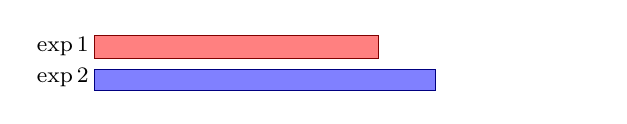
\begin{tikzpicture}[scale=0.4]
	\draw[color=white] (-2, -3) -- (16, -3);
	\node[font=\footnotesize] (e1) at (-1, -3.3) {$\exp{1}$};
	\node[font=\footnotesize] (e2) at (-1, -4.3) {$\exp{2}$};
	\filldraw[fill=red!50!white, draw=red!50!black] (0, -3.7) rectangle (9.02554, -2.9623);
	\filldraw[fill=blue!50!white, draw=blue!50!black] (0, -4.7) rectangle (10.8307, -4.04426);
\end{tikzpicture}
\end{center}
}

%\vspace{.05cm}

\uncover<3->{
\begin{center}
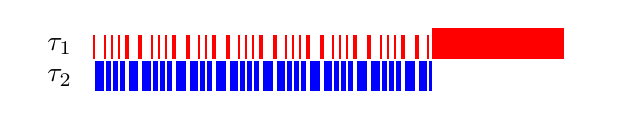
\begin{tikzpicture}[scale=0.4]
		\draw[color=white] (-2, -1) -- (16, -1);
% \draw[->] (-.2, -3.2) -- (15.2, -3.2) node[right] {time};
\node[] (t1) at (-1, -1.3) {$\tau_1$};
\node[] (t1) at (-1, -2.3) {$\tau_2$};
\fill[red] (0.0665893, -1.7) rectangle (0.130345, -0.929508);
\fill[blue] (0.130345, -2.7) rectangle (0.393197, -1.76557);
\fill[red] (0.393197, -1.7) rectangle (0.456953, -0.929508);
\fill[blue] (0.456953, -2.7) rectangle (0.614665, -1.76557);
\fill[red] (0.614665, -1.7) rectangle (0.67842, -0.929508);
\fill[blue] (0.67842, -2.7) rectangle (0.836132, -1.76557);
\fill[red] (0.836132, -1.7) rectangle (0.899887, -0.929508);
\fill[blue] (0.899887, -2.7) rectangle (1.0576, -1.76557);
\fill[red] (1.0576, -1.7) rectangle (1.18511, -0.929508);
\fill[blue] (1.18511, -2.7) rectangle (1.50053, -1.76557);
\fill[red] (1.50053, -1.7) rectangle (1.62804, -0.929508);
\fill[blue] (1.62804, -2.7) rectangle (1.8909, -1.76557);
\fill[red] (1.8909, -1.7) rectangle (1.95465, -0.929508);
\fill[blue] (1.95465, -2.7) rectangle (2.11236, -1.76557);
\fill[red] (2.11236, -1.7) rectangle (2.17612, -0.929508);
\fill[blue] (2.17612, -2.7) rectangle (2.33383, -1.76557);
\fill[red] (2.33383, -1.7) rectangle (2.39759, -0.929508);
\fill[blue] (2.39759, -2.7) rectangle (2.5553, -1.76557);
\fill[red] (2.5553, -1.7) rectangle (2.68281, -0.929508);
\fill[blue] (2.68281, -2.7) rectangle (2.99823, -1.76557);
\fill[red] (2.99823, -1.7) rectangle (3.12574, -0.929508);
\fill[blue] (3.12574, -2.7) rectangle (3.3886, -1.76557);
\fill[red] (3.3886, -1.7) rectangle (3.45235, -0.929508);
\fill[blue] (3.45235, -2.7) rectangle (3.61006, -1.76557);
\fill[red] (3.61006, -1.7) rectangle (3.67382, -0.929508);
\fill[blue] (3.67382, -2.7) rectangle (3.83153, -1.76557);
\fill[red] (3.83153, -1.7) rectangle (3.95904, -0.929508);
\fill[blue] (3.95904, -2.7) rectangle (4.27447, -1.76557);
\fill[red] (4.27447, -1.7) rectangle (4.40198, -0.929508);
\fill[blue] (4.40198, -2.7) rectangle (4.66483, -1.76557);
\fill[red] (4.66483, -1.7) rectangle (4.72858, -0.929508);
\fill[blue] (4.72858, -2.7) rectangle (4.8863, -1.76557);
\fill[red] (4.8863, -1.7) rectangle (4.95005, -0.929508);
\fill[blue] (4.95005, -2.7) rectangle (5.10776, -1.76557);
\fill[red] (5.10776, -1.7) rectangle (5.17152, -0.929508);
\fill[blue] (5.17152, -2.7) rectangle (5.32923, -1.76557);
\fill[red] (5.32923, -1.7) rectangle (5.45674, -0.929508);
\fill[blue] (5.45674, -2.7) rectangle (5.77216, -1.76557);
\fill[red] (5.77216, -1.7) rectangle (5.89968, -0.929508);
\fill[blue] (5.89968, -2.7) rectangle (6.16253, -1.76557);
\fill[red] (6.16253, -1.7) rectangle (6.22628, -0.929508);
\fill[blue] (6.22628, -2.7) rectangle (6.384, -1.76557);
\fill[red] (6.384, -1.7) rectangle (6.44775, -0.929508);
\fill[blue] (6.44775, -2.7) rectangle (6.60546, -1.76557);
\fill[red] (6.60546, -1.7) rectangle (6.66922, -0.929508);
\fill[blue] (6.66922, -2.7) rectangle (6.82693, -1.76557);
\fill[red] (6.82693, -1.7) rectangle (6.95444, -0.929508);
\fill[blue] (6.95444, -2.7) rectangle (7.26986, -1.76557);
\fill[red] (7.26986, -1.7) rectangle (7.39738, -0.929508);
\fill[blue] (7.39738, -2.7) rectangle (7.66023, -1.76557);
\fill[red] (7.66023, -1.7) rectangle (7.72398, -0.929508);
\fill[blue] (7.72398, -2.7) rectangle (7.8817, -1.76557);
\fill[red] (7.8817, -1.7) rectangle (7.94545, -0.929508);
\fill[blue] (7.94545, -2.7) rectangle (8.10316, -1.76557);
\fill[red] (8.10316, -1.7) rectangle (8.16692, -0.929508);
\fill[blue] (8.16692, -2.7) rectangle (8.32463, -1.76557);
\fill[red] (8.32463, -1.7) rectangle (8.45214, -0.929508);
\fill[blue] (8.45214, -2.7) rectangle (8.76756, -1.76557);
\fill[red] (8.76756, -1.7) rectangle (8.89508, -0.929508);
\fill[blue] (8.89508, -2.7) rectangle (9.15793, -1.76557);
\fill[red] (9.15793, -1.7) rectangle (9.22168, -0.929508);
\fill[blue] (9.22168, -2.7) rectangle (9.3794, -1.76557);
\fill[red] (9.3794, -1.7) rectangle (9.44315, -0.929508);
\fill[blue] (9.44315, -2.7) rectangle (9.60086, -1.76557);
\fill[red] (9.60086, -1.7) rectangle (9.66462, -0.929508);
\fill[blue] (9.66462, -2.7) rectangle (9.82233, -1.76557);
\fill[red] (9.82233, -1.7) rectangle (9.94984, -0.929508);
\fill[blue] (9.94984, -2.7) rectangle (10.2653, -1.76557);
\fill[red] (10.2653, -1.7) rectangle (10.3928, -0.929508);
\fill[blue] (10.3928, -2.7) rectangle (10.6556, -1.76557);
\fill[red] (10.6556, -1.7) rectangle (10.7194, -0.929508);
\fill[blue] (10.7194, -2.7) rectangle (10.8245, -1.76557);
\fill[red] (10.8245, -1.7) rectangle (15, -0.7);
\end{tikzpicture}
\end{center}
}



%\vspace{.05cm}

\uncover<4->{
\begin{center}
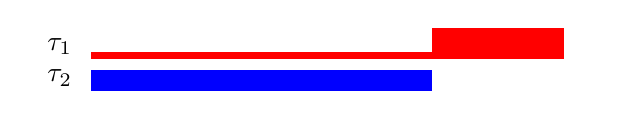
\begin{tikzpicture}[scale=0.4]
		\draw[color=white] (-2, -1) -- (16, -1);
% \draw[color=red, line width=2pt] (0,0) edge (9.02554,1.66572);
% \draw[color=red, line width=2pt] (9.02554,1.66572) edge (10.8307,1.515);
% \draw[color=red, line width=2pt] (10.8307,1.515) edge (15,0);
% \draw[color=blue, line width=2pt] (0,0) edge (9.02554,0);
% \draw[color=blue, line width=2pt] (9.02554,0) edge (10.8307,0);
% \draw[color=blue, line width=2pt] (10.8307,0) edge (15,0);
% \draw[color=black, line width=2pt] (0,0) edge (9.02554,2.90417);
% \draw[color=black, line width=2pt] (9.02554,2.90417) edge (10.8307,3.485);
% \draw[color=black, line width=2pt] (10.8307,3.485) edge (15,5);
\node[] (t1) at (-1, -1.3) {$\tau_1$};
\node[] (t1) at (-1, -2.3) {$\tau_2$};
% \draw[] (15.2, 5.2) node[right] {$m_m$};
% \draw[->] (-.2, -.2) -- (15.2, -.2) node[right] {time};
% \draw[->] (-.2, -.2) -- (-.2, 5.2) node[right] {memory};
% \draw[step=35.8423,very thin,color=gray] (0,0) grid (15, 5);
\fill[blue] (0, -2.7) rectangle (9.02554, -2.04426);
\fill[red] (0, -1.7) rectangle (9.02554, -1.4702);
\fill[blue] (9.02554, -2.7) rectangle (10.8307, -2.04426);
\fill[red] (9.02554, -1.7) rectangle (10.8307, -1.4702);
\fill[red] (10.8307, -1.7) rectangle (15, -0.7);
\end{tikzpicture}
\end{center}
}

\end{columns}


\end{frame}


\begin{frame}[fragile]
	\frametitle{Checking the Constraint}

\begin{center}
\begin{tikzpicture}[scale = 0.55]


%\draw (8.6353, -6.5) rectangle (15, -1);




\filldraw[fill=red!50!white, draw=red!50!black] (0, -4) rectangle (1.68224, -3.85714);
\filldraw[fill=green!50!white, draw=green!50!black] (0.841121, -6) rectangle (2.24299, -5.08571);
\filldraw[fill=red!50!white, draw=red!50!black] (4.48598, -4) rectangle (6.72897, -3.85714);
\filldraw[fill=blue!50!white, draw=blue!50!black] (5.04673, -5) rectangle (8.41121, -4.46429);
\filldraw[fill=green!50!white, draw=green!50!black] (7.85047, -6) rectangle (10.0935, -5.10714);
\filldraw[fill=red!50!white, draw=red!50!black] (7.57009, -4) rectangle (10.3738, -3.85714);
\filldraw[fill=blue!50!white, draw=blue!50!black] (9.25234, -5) rectangle (12.0561, -4.57143);
\filldraw[fill=green!50!white, draw=green!50!black] (11.215, -6) rectangle (12.6168, -5.08571);

\draw[->] (-.2, -.2) -- (15.2, -.2) node[right] {{\footnotesize time}};
\draw[->] (-.2, -.2) -- (-.2, 5.2) node[right] {{\footnotesize memory}};
\draw[step=46.9484,very thin,color=gray] (0,0) grid (15, 5);


\node[] (e1) at (-1, -4) {\scriptsize{$\exp{1}$}};
\node[] (e2) at (-1, -4.7) {\scriptsize{$\exp{2}$}};
\node[] (e3) at (-1, -5.6) {\scriptsize{$\exp{3}$}};


\uncover<1-> {


\node[] (t1) at (-1, -1.5) {\scriptsize{$\tau_1$}};

\draw[color=black, line width=1.5pt] (0,0) edge (0.841121,0.0704225);
\draw[color=green, line width=1.5pt] (0,0) edge (0.841121,0);
\draw[color=blue, line width=1.5pt] (0,0) edge (0.841121,0);
\draw[color=red, line width=1.5pt] (0,0) edge (0.841121,0);
\fill[red] (0, -1.7) rectangle (0.841121, -1.53607);
\only<1-3> \draw[dashed] (0.841121, -1) -- (0.841121, -6.5);

}
\uncover<2-> {


\node[] (t3) at (-1, -3.2) {\scriptsize{$\tau_3$}};

\draw[color=black, line width=1.5pt] (0.841121,0.0704225) edge (1.68224,0.413763);
\draw[color=green, line width=1.5pt] (0.841121,0) edge (1.68224,0.177786);
\draw[color=blue, line width=1.5pt] (0.841121,0) edge (1.68224,0);
\draw[color=red, line width=1.5pt] (0.841121,0) edge (1.68224,0);
\fill[red] (0.841121, -1.7) rectangle (1.68224, -1.53607);
\fill[green] (0.841121, -3.7) rectangle (1.68224, -3.06468);
\only<2-4> \draw[dashed] (1.68224, -1) -- (1.68224, -6.5);

}
\uncover<3-> {

\draw[color=black, line width=1.5pt] (1.68224,0.413763) edge (2.24299,0.634421);
\draw[color=green, line width=1.5pt] (1.68224,0.177786) edge (2.24299,0.257598);
\draw[color=blue, line width=1.5pt] (1.68224,0) edge (2.24299,0);
\draw[color=red, line width=1.5pt] (1.68224,0) edge (2.24299,0);
\fill[green] (1.68224, -3.7) rectangle (2.24299, -2.92951);
\only<3-5> \draw[dashed] (2.24299, -1) -- (2.24299, -6.5);

}
\uncover<4-> {

\draw[color=black, line width=1.5pt] (2.24299,0.634421) edge (2.89761,0.892019);
\draw[color=green, line width=1.5pt] (2.24299,0.257598) edge (2.89761,0);
\draw[color=blue, line width=1.5pt] (2.24299,0) edge (2.89761,0);
\draw[color=red, line width=1.5pt] (2.24299,0) edge (2.89761,0);
\fill[green] (2.24299, -3.7) rectangle (2.89761, -2.92951);
\only<4-6> \draw[dashed] (2.89761, -1) -- (2.89761, -6.5);

}
\uncover<5-> {

\draw[color=black, line width=1.5pt] (2.89761,0.892019) edge (4.48598,0.892019);
\draw[color=green, line width=1.5pt] (2.89761,0) edge (4.48598,0);
\draw[color=blue, line width=1.5pt] (2.89761,0) edge (4.48598,0);
\draw[color=red, line width=1.5pt] (2.89761,0) edge (4.48598,0);
\only<5-7> \draw[dashed] (4.48598, -1) -- (4.48598, -6.5);

}
\uncover<6-> {

\draw[color=black, line width=1.5pt] (4.48598,0.892019) edge (5.04673,0.938967);
\draw[color=green, line width=1.5pt] (4.48598,0) edge (5.04673,0);
\draw[color=blue, line width=1.5pt] (4.48598,0) edge (5.04673,0);
\draw[color=red, line width=1.5pt] (4.48598,0) edge (5.04673,0);
\fill[red] (4.48598, -1.7) rectangle (5.04673, -1.53607);
\only<6-8> \draw[dashed] (5.04673, -1) -- (5.04673, -6.5);

}
\uncover<7-> { 

\node[] (t2) at (-1, -2.4) {\scriptsize{$\tau_2$}};

\draw[color=black, line width=1.5pt] (5.04673,0.938967) edge (6.72897,1.5455);
\draw[color=green, line width=1.5pt] (5.04673,0) edge (6.72897,0);
\draw[color=blue, line width=1.5pt] (5.04673,0) edge (6.72897,0.0624813);
\draw[color=red, line width=1.5pt] (5.04673,0) edge (6.72897,0);
\fill[red] (5.04673, -1.7) rectangle (6.72897, -1.53607);
\fill[blue] (5.04673, -2.7) rectangle (6.72897, -2.15797);
\only<7-9> \draw[dashed] (6.72897, -1) -- (6.72897, -6.5);


}
\uncover<8-> {

\draw[color=black, line width=1.5pt] (6.72897,1.5455) edge (7.57009,1.84127);
\draw[color=green, line width=1.5pt] (6.72897,0) edge (7.57009,0);
\draw[color=blue, line width=1.5pt] (6.72897,0.0624813) edge (7.57009,0.0307911);
\draw[color=red, line width=1.5pt] (6.72897,0) edge (7.57009,0);
\fill[blue] (6.72897, -2.7) rectangle (7.57009, -2.01148);
\only<8-10> \draw[dashed] (7.57009, -1) -- (7.57009, -6.5);

}
\uncover<9-> {

\draw[color=black, line width=1.5pt] (7.57009,1.84127) edge (7.85047,1.94236);
\draw[color=green, line width=1.5pt] (7.57009,0) edge (7.85047,0);
\draw[color=blue, line width=1.5pt] (7.57009,0.0307911) edge (7.85047,0.0412047);
\draw[color=red, line width=1.5pt] (7.57009,0) edge (7.85047,0);
\fill[red] (7.57009, -1.7) rectangle (7.85047, -1.53607);
\fill[blue] (7.57009, -2.7) rectangle (7.85047, -2.15797);
\only<9-11> \draw[dashed] (7.85047, -1) -- (7.85047, -6.5);

}
\uncover<10-> {

\draw[color=black, line width=1.5pt] (7.85047,1.94236) edge (8.41121,2.14454);
\draw[color=green, line width=1.5pt] (7.85047,0) edge (8.41121,0.293427);
\draw[color=blue, line width=1.5pt] (7.85047,0.0412047) edge (8.41121,0.0620318);
\draw[color=red, line width=1.5pt] (7.85047,0) edge (8.41121,0);
\fill[red] (7.85047, -1.7) rectangle (8.41121, -1.53607);
\fill[blue] (7.85047, -2.7) rectangle (8.41121, -2.15797);
\only<10-12> \draw[dashed] (8.41121, -1) -- (8.41121, -6.5);

}
\uncover<11-> {

\draw[color=black, line width=1.5pt] (8.41121,2.14454) edge (8.6353,2.22533);
\draw[color=green, line width=1.5pt] (8.41121,0.293427) edge (8.6353,0.410685);
\draw[color=blue, line width=1.5pt] (8.41121,0.0620318) edge (8.6353,0);
\draw[color=red, line width=1.5pt] (8.41121,0) edge (8.6353,0);
\fill[red] (8.41121, -1.7) rectangle (8.6353, -1.53607);
\fill[blue] (8.41121, -2.7) rectangle (8.6353, -2.15797);
\only<11-13> \draw[dashed] (8.6353, -1) -- (8.6353, -6.5);

}
\uncover<12-> {

\draw[color=black, line width=1.5pt] (8.6353,2.22533) edge (9.25234,2.43154);
\draw[color=green, line width=1.5pt] (8.6353,0.410685) edge (9.25234,0.579024);
\draw[color=blue, line width=1.5pt] (8.6353,0) edge (9.25234,0);
\draw[color=red, line width=1.5pt] (8.6353,0) edge (9.25234,0);
\fill[red] (8.6353, -1.7) rectangle (9.25234, -1.53607);
\fill[green] (8.6353, -3.7) rectangle (9.25234, -3.20959);
\only<12-14> \draw[dashed] (9.25234, -1) -- (9.25234, -6.5);

}
\uncover<13-> {

\draw[color=black, line width=1.5pt] (9.25234,2.43154) edge (10.0935,2.73275);
\draw[color=green, line width=1.5pt] (9.25234,0.579024) edge (10.0935,0.999643);
\draw[color=blue, line width=1.5pt] (9.25234,0) edge (10.0935,0);
\draw[color=red, line width=1.5pt] (9.25234,0) edge (10.0935,0);
\fill[red] (9.25234, -1.7) rectangle (10.0935, -1.53607);
\fill[blue] (9.25234, -2.7) rectangle (10.0935, -2.2082);
\fill[green] (9.25234, -3.7) rectangle (10.0935, -3.65456);
\only<13-15> \draw[dashed] (10.0935, -1) -- (10.0935, -6.5);

}
\uncover<14-> {

\draw[color=black, line width=1.5pt] (10.0935,2.73275) edge (10.3738,2.83315);
\draw[color=green, line width=1.5pt] (10.0935,0.999643) edge (10.3738,0.993136);
\draw[color=blue, line width=1.5pt] (10.0935,0) edge (10.3738,0);
\draw[color=red, line width=1.5pt] (10.0935,0) edge (10.3738,0);
\fill[red] (10.0935, -1.7) rectangle (10.3738, -1.53607);
\fill[blue] (10.0935, -2.7) rectangle (10.3738, -2.2082);
\fill[green] (10.0935, -3.7) rectangle (10.3738, -3.65456);
\only<14-16> \draw[dashed] (10.3738, -1) -- (10.3738, -6.5);

}
\uncover<15-> {

\draw[color=black, line width=1.5pt] (10.3738,2.83315) edge (11.215,3.20121);
\draw[color=green, line width=1.5pt] (10.3738,0.993136) edge (11.215,0.836353);
\draw[color=blue, line width=1.5pt] (10.3738,0) edge (11.215,0);
\draw[color=red, line width=1.5pt] (10.3738,0) edge (11.215,0);
\fill[blue] (10.3738, -2.7) rectangle (11.215, -2.2082);
\fill[green] (10.3738, -3.7) rectangle (11.215, -3.33503);
\only<15-17> \draw[dashed] (11.215, -1) -- (11.215, -6.5);

}
\uncover<16-> {

\draw[color=black, line width=1.5pt] (11.215,3.20121) edge (12.0561,3.56926);
\draw[color=green, line width=1.5pt] (11.215,0.836353) edge (12.0561,1.13027);
\draw[color=blue, line width=1.5pt] (11.215,0) edge (12.0561,0);
\draw[color=red, line width=1.5pt] (11.215,0) edge (12.0561,0);
\fill[blue] (11.215, -2.7) rectangle (12.0561, -2.2082);
\fill[green] (11.215, -3.7) rectangle (12.0561, -3.33503);
\only<16-18> \draw[dashed] (12.0561, -1) -- (12.0561, -6.5);

}
\uncover<17-> {

\draw[color=black, line width=1.5pt] (12.0561,3.56926) edge (12.6168,3.85564);
\draw[color=black, line width=1.5pt] (12.6168,3.85564) edge (14.8575,5);
\draw[color=green, line width=1.5pt] (12.0561,1.13027) edge (12.6168,1.14436);
\draw[color=green, line width=1.5pt] (12.6168,1.14436) edge (14.8575,0);
\draw[color=blue, line width=1.5pt] (12.0561,0) edge (12.6168,0);
\draw[color=blue, line width=1.5pt] (12.6168,0) edge (14.8575,0);
\draw[color=red, line width=1.5pt] (12.0561,0) edge (12.6168,0);
\draw[color=red, line width=1.5pt] (12.6168,0) edge (14.8575,0);
\fill[green] (12.0561, -3.7) rectangle (14.8575, -2.7);

}

\end{tikzpicture}
\end{center}
% \uncover<5->{
% \begin{itemize}
% 	\item We can jump from \memph{"event"} to \memph{"event"}: \memph{$O(n \log n)$} worst case time complexity
% \end{itemize}
% }

\end{frame}



\begin{frame}[fragile]
  \frametitle{Sweep algorithm~\mycite{BeldiceanuCarlsson01}}
    
		\begin{itemize}
			\item The constraint can be checked in $\memph{O(n \log n)}$
			\pause \item Several experiments active simultaneously:
			\begin{itemize}
				\item Error is less than or equal to \memph{$1 + \frac{\tau^{max}}{\tau^{min}} \simeq 3$} blocks \\~
			\end{itemize}			
			\pause \item \memph{Faster and more accurate than the reservoir/transfer tasks model}
			
			\pause \item Bound adjustments? Two principles:
			\begin{itemize}
				\item Producing too much data too quickly can lead to data loss
				\item Filling up the mass memory while not in visibility can lead to data loss
			\end{itemize}
		\end{itemize}
	
\end{frame}


	\def\tsat{\overline{t}}


\begin{frame}[fragile]
\frametitle{Propagation: production/transfer rate}
\begin{myblock}{For a set of tasks}
\begin{itemize}
\item \memph{lower bound} on how much time the CDMS needs to transfer without data loss
\end{itemize}
\end{myblock}

\medskip

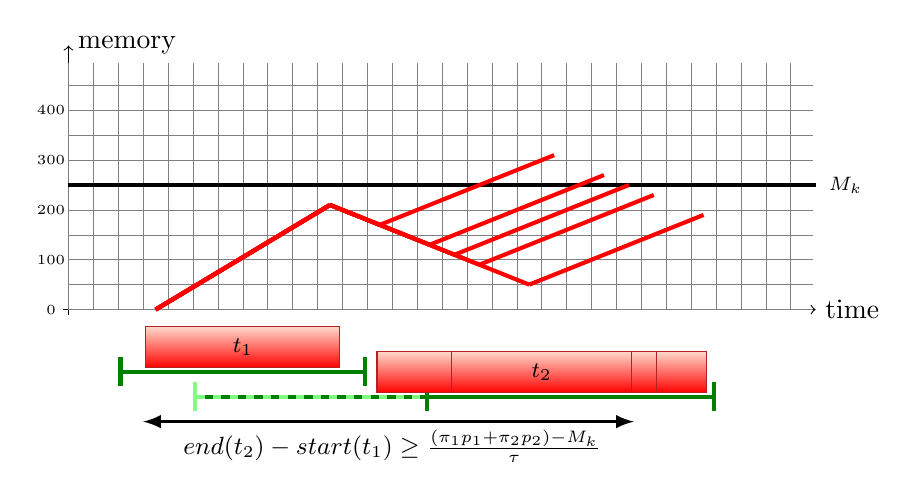
\begin{tikzpicture}[scale=0.9]
	
\tikzset{task/.style={draw=FireBrick,top color=OrangeRed!20, bottom color=Red, minimum height=15pt, shape=rectangle, font=\footnotesize}}
\tikzset{t1/.style={task, minimum width=70pt}}
\tikzset{t2/.style={task, minimum width=65pt}}
	
\node[t1] (t31) at (70pt,-15pt) {$t_1$};
\draw[|-|, ultra thick, green!50!black] (20pt,-25pt) -- (120pt,-25pt);

\uncover<1-4> {
\draw[|-|, ultra thick, green!50!black] (50pt,-35pt) -- (260pt,-35pt);
}

\uncover<5> {
\draw[|-, dashed, ultra thick, green!50] (50pt,-35pt) -- (143pt,-35pt);
\draw[|-|, ultra thick, green!50!black] (143pt,-35pt) -- (260pt,-35pt);
}

\draw[->] (-2pt,0pt) -- (300pt,0pt) node[right] {time};
\draw[->] (0pt,-2pt) -- (0pt,106pt) node[right] {memory};
\draw[step=10pt,very thin,color=gray] (0pt,0pt) grid (299pt,99pt);
\node[] (mark0) at (-7pt,0pt) {{\tiny 0}};
\node[] (mark20) at (-7pt,20pt) {{\tiny 100}};
\node[] (mark40) at (-7pt,40pt) {{\tiny 200}};
\node[] (mark60) at (-7pt,60pt) {{\tiny 300}};
\node[] (mark80) at (-7pt,80pt) {{\tiny 400}};

\draw[color=black, line width=1.5pt] (0pt,50pt) edge (300pt,50pt);
\node[] (mark0) at (312pt,50pt) {{\scriptsize $M_k$}};

\uncover<1>{
\node[t2] (t32) at (220pt,-25pt) {$t_2$};
\draw[color=red, line width=1.5pt] (35pt,0pt) edge (105pt,42pt);
\draw[color=red, line width=1.5pt] (105pt,42pt) edge (185pt,10pt);
\draw[color=red, line width=1.5pt] (185pt,10pt) edge (255pt,38pt);
}

\uncover<2>{
\node[t2] (t32) at (200pt,-25pt) {$t_2$};
\draw[color=red, line width=1.5pt] (35pt,0pt) edge (105pt,42pt);
\draw[color=red, line width=1.5pt] (105pt,42pt) edge (165pt,18pt);
\draw[color=red, line width=1.5pt] (165pt,18pt) edge (235pt,46pt);
}

\uncover<3>{
\node[t2] (t32) at (180pt,-25pt) {$t_2$};
\draw[color=red, line width=1.5pt] (35pt,0pt) edge (105pt,42pt);
\draw[color=red, line width=1.5pt] (105pt,42pt) edge (145pt,26pt);
\draw[color=red, line width=1.5pt] (145pt,26pt) edge (215pt,54pt);
}

\uncover<4>{
\node[t2] (t32) at (160pt,-25pt) {$t_2$};
\draw[color=red, line width=1.5pt] (35pt,0pt) edge (105pt,42pt);
\draw[color=red, line width=1.5pt] (105pt,42pt) edge (125pt,34pt);
\draw[color=red, line width=1.5pt] (125pt,34pt) edge (195pt,62pt);
}


\uncover<5>{
\node[t2] (t32) at (190pt,-25pt) {$t_2$};
\draw[color=red, line width=1.5pt] (35pt,0pt) edge (105pt,42pt);
\draw[color=red, line width=1.5pt] (105pt,42pt) edge (155pt,22pt);
\draw[color=red, line width=1.5pt] (155pt,22pt) edge (225pt,50pt);

\draw[latex-latex, very thick] (30pt,-45pt) -- (227pt,-45pt);
\node[] (mark0) at (130pt,-55pt) {{\small \memph{$end(t_2) - start(t_1) \geq \frac{(\pi_1 p_1 + \pi_2 p_2)-M_k}{\tau}$}}};
}


\end{tikzpicture}

\end{frame}


\begin{frame}
	\frametitle{Propagation: production/transfer rate}
	
	More generally, we consider a set of tasks \memph{$\Omega$} of a given experiment
	\begin{itemize}
		%\item Let \memph{$[a,b]=[\min_{t_{ki}\in \Omega}(\max(s_{ki})), \max_{t_{ki}\in \Omega}(\min(s_{ki}+p_{ki}))]$}
		\pause \item Let \memph{$[a,b]$} be a time interval \memph{necessarily} contained in \memph{$\Omega$}'s transfer period 
		\pause \item We can take into account the tasks of higher priority producing during \memph{$[a,b]$}
	\end{itemize}
	
\pause \begin{myblock}{Filtering rule}
\begin{itemize}
%\item Let \memph{$min(|t_{ki}\cap[a,b]|)$} be the minimal intersection between \memph{$t_{ki}$} and \memph{$[a,b]$}
\item 
Minimum amount of higher priority data to transfer on \memph{$[a,b]$} over transfer rate:
\begin{itemize}
	\item Lower bound on the time dedicated to higher priority experiment: \memph{$T_k(a,b)$}
\end{itemize}
% \begin{itemize}
% 	\item \memph{$\sum_{j=1}^{j<R(k)} \sum_{i=1}^n \min(|t_{P(j)i} \cap [a,b]|)*\pi_{P(j)i}$}
% \end{itemize}
% \pause
% \item Necessary duration:\\
% \hspace{1cm} \memph{$T_k(a,b)= \dfrac{\sum_{j=1}^{j<R(k)} \sum_{i=1}^n \min(|t_{P(j)i} \cap [a,b]|)*\pi_{P(j)i}}{\tau}$}
\pause 
\item Induced constraint:\\
\hspace{1cm} \memph{$Makespan(\Omega) \geq \frac{(\sum_{t_{ki}\in \Omega} \pi_i p_i)-M_k}{\tau} + T_k(a,b)$}
%\memph{$\max_{t_{ki} \in \Omega}(e_{ki}) - \min_{t_{ki} \in \Omega}(s_{ki}) \geq \frac{(\sum_{t_{ki}\in \Omega} \pi_i p_i)-M_k}{\tau} + T_k(a,b)$}

\end{itemize}
\end{myblock}

\end{frame}

	
	
\begin{frame}
  \frametitle{Propagation: visibility}
  
	
	\begin{itemize}
		\item When the mass memory is full, no more data is transferred to it
		\uncover<2->{\item Minimal usage and peak \memph{$m_0^{max}$}
%		\item Compute the date \memph{$\tsat$} at which the usage reaches its maximum \memph{$m_0^{\tsat}$}
		\uncover<3->{%\item Given an experiment with memory \memph{$M_k$}
		%\begin{itemize}
			\item If the production exceeds \memph{$M_k + M_0 - m_0^{max}$} in \memph{$[a, b]$} then data will be \memph{lost}
		%\end{itemize}
		\uncover<4->{
		\begin{itemize}
			\item \memph{Filtering: bound start time w.r.t. this quantity of data and production rate}
		\end{itemize}
		}
		}
		}
	\end{itemize}


\begin{center}
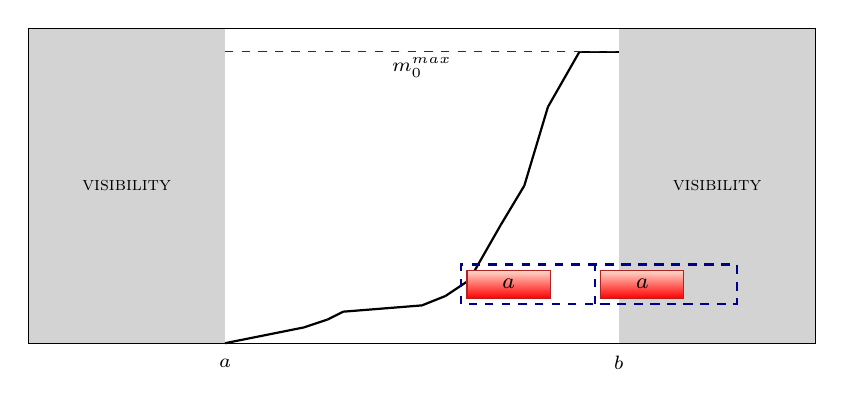
\begin{tikzpicture}
	
	\tikzset{task/.style={draw=FireBrick,top color=OrangeRed!20, bottom color=Red, minimum height=10pt, shape=rectangle, font=\footnotesize, minimum width=30pt}}
	
		 
		 \fill[color=LightGray] (0,0) rectangle (2.5,4);
		 \node[font=\scriptsize] at (1.25,2) {{\sc visibility}};
		 \fill[color=LightGray] (7.5,0) rectangle (10,4);
		 \node[font=\scriptsize] at (8.75,2) {{\sc visibility}};
		 \draw[color=black] (0,0) rectangle (10,4);
		 
		 \uncover<2-> {
		 \draw[thick] (2.5,0) -- (3.5,.2);
		 \draw[thick] (3.5,.2) -- (3.8,.3);
		 \draw[thick] (3.8,.3) -- (4,.4);
		 \draw[thick] (4,.4) -- (5,.48);
		 \draw[thick] (5,.48) -- (5.3,.6);
		 \draw[thick] (5.3,.6) -- (5.6,.8);
		 \draw[thick] (5.6,.8) -- (6,1.5);
		 \draw[thick] (6,1.5) -- (6.3,2);
		 \draw[thick] (6.3,2) -- (6.6,3);
		 \draw[thick] (6.6,3) -- (7,3.7);
		 \draw[thick] (7,3.7) -- (7.5,3.7);
		 
		 %\draw[dashed, color=red!60!black] (7,0) -- (7,4);
		 
		 \draw[dashed, color=red!60!black] (2.5,3.7) -- (7.5,3.7);
		 
%		 \node[font=\scriptsize] at (7, -.2) {$\tsat$};
		 \node[font=\scriptsize] at (2.5, -.25) {$a$};
		 \node[font=\scriptsize] at (7.5, -.25) {$b$};
		 \node[font=\scriptsize] at (5, 3.5) {\memph{$m_0^{max}$}};
		 }
		 
		 
		 \uncover<3> {
		 \draw[dashed, color=DarkBlue, thick] (5.5,.5) rectangle (9,1);
		 \node[task] at (6.1,.75) {$a$};
		 }
		 
		 \uncover<4> {
		 \draw[dashed, color=DarkBlue, thick] (7.2,.5) rectangle (9,1);
		 \node[task] at (7.8,.75) {$a$};
		 }
		 
				 
\end{tikzpicture}
\end{center}


\end{frame}






















% \section{Single Machine Resource}
%
% % \input{src/sections/unary.tex}
%
% \section{Cumulative Resource}

% \input{src/sections/cumulative.tex}

% \section{Search}

% \section{Precedence Graph}

		
% 1/ Precedence graph / difference system -> convenient way of implementing	domains
		
% 1/ CP branching does not work
% 2/ Schedule or postpone is good but not great and not standard branching
% 3/ Idea of branching on precedences
% 4/ Branching on precedences performs surprisingly well
% 5/ Some explanation ?
% 6/ Precedence graph / difference system -> convenient way of implementing this
		
		
% \begin{frame}
% 	\frametitle{Search}
%
% 	\begin{itemize}
% 		\item
% 		\begin{itemize}
% 			\item Choose task $i$ minimizing $\lct{i} - \est{i} - \dur{i}$ (and/or most constrained by resources and precedences)
% 			\item Set $\stof{i}$ to $\est{i}$
% 			\item When backtracking, set $\stof{i}$ to $\est{i}+1$
% 		\end{itemize}
% 		\item ``Schedule or postpone'' $\simeq$ branch on the task to start at the first available slot
% 		\begin{itemize}
% 			\item Circumvent the precision problem, usually efficient for makespan minimization
% 			\item Non trivial to implement in a classical CP solver
% 			\item Might be incomplete for some objectives or constraints
% 		\end{itemize}
% 	\end{itemize}
%
% \end{frame}


\begin{frame}
	\frametitle{The importance of search: a short story}

	\begin{columns}
	\begin{column}{0.5\textwidth}
		
		\only<1-2> {
			\begin{itemize}
				\item Jobs: Files to transfer
				\item Resources:
				\begin{itemize}
					\item \memph{Download channels}: at most that many simultaneous downloads
					\uncover<2-> {
					\begin{itemize}
						\item \emph{Cumulative resource shared by every task}
					\end{itemize}
					}
					\item \memph{Memory banks}: cannot download two files stored on the same memory bank simultaneously
					\uncover<2-> {
					\begin{itemize}
						\item \emph{Tasks partitioned in as many unary resources as memory banks (\memph{$m$})}
					\end{itemize}
					}
				\end{itemize}
				\item Download as much data as possible within a given time window
				\uncover<2-> {
				\begin{itemize}
					\item \emph{Minimize makespan}
				\end{itemize}
				}
			\end{itemize}
			}
			
			\only<3-> {
				\begin{itemize}
					\item Alas, our method was hardly better than a very basic greedy algorithm...
				\end{itemize}
			
				\begin{myblock}{Greedy algorithm}
					\begin{itemize}
						\item \textbf{Repeat:}
						\begin{itemize}
						\item Choose the largest task \memph{a} from the resource with highest demand
						\item Schedule \memph{a} as soon as possible
						\end{itemize}
					\end{itemize}
				\end{myblock}
			
				\uncover<4->{
				% \begin{myblock}{Approximation ratio}
					\begin{itemize}
						\item Approximation ratio: \memph{$ 2 - \frac{2}{m+1} $} \mycite{HebrardEtAl16}
						\uncover<5->{
						\item Approximation ratio: \memph{$ 1 + \rho \frac{m-1}{n} $} where \memph{$\rho$} is the ratio between largest and smallest task size
						}
					\end{itemize}
				% \end{myblock}
				}
				
				\uncover<6->{
					Not \memph{all} resource scheduling are hard!
				}
			}

	\end{column}
	\begin{column}{0.5\textwidth}  %%<--- here
		
		\begin{center}

	     \includegraphics[width=0.8\textwidth]{im/satellites.jpg}
			 
			 \includegraphics[width=0.8\textwidth]{im/station.jpg}

		\end{center}
		
	\end{column}
	\end{columns}
	

\end{frame}

		

\begin{frame}
	\frametitle{Search strategy}

	\begin{itemize}
		\item Default CP strategy is a very bad idea:
		\begin{itemize}
			\item Choose task \memph{$i$} minimizing \memph{$\lct{i} - \est{i} - \dur{i}$} (and/or most constrained by resources and precedences)
			\item Branch on \memph{$\stof{i} = \est{i}$ or $\stof{i} > \est{i}$}: create ``holes'', dependent on the precision
			% \item When backtracking, set $\stof{i}$ to $\est{i}+1$
		\end{itemize}
		\item ``Schedule or postpone'' $\simeq$ branch on the task to start at the first available slot
		\begin{itemize}
			\item Circumvent the precision problem, usually efficient for makespan minimization
			\item Non trivial to implement in a classical CP solver
			\item Might be incomplete for some objectives or constraints
		\end{itemize}
		\item Sophisticated techniques in the latest CP solver (CP Optimizer) \mycite{VilimEtAl15}
		\begin{itemize}
			\item Alternate between Large Neighborhood Search and ``Failure Directed Search''
		\end{itemize}
	\end{itemize}

	% \begin{myblock}{Branch on precedences \mycitation{Cesta and Odi}}
	% 	\begin{itemize}
	% 		\item For unary resources: one Boolean variable per disjunctive constraint
	% 	\end{itemize}
	% \end{myblock}

\end{frame}


\newcommand{\bestopt}[1]{\cellcolor{bostonuniversityred}{\bf \textcolor{white}{#1}}}
\newcommand{\best}[1]{\cellcolor{airforceblue}{\bf \textcolor{white}{#1}}}



\begin{frame}
	\frametitle{Precedence graph / Difference system}

	\begin{center}
		\begin{colorschedfigure}{.5}
			\input{ex/scheduling_instance.tex}
		\end{colorschedfigure}


		\begin{colorschedfigure}{.55}
			\input{ex/precedence_graph.tex}
		\end{colorschedfigure}
	\end{center}
\end{frame}


\begin{frame}
	\frametitle{Precedence graph as ``domain''}

	\begin{center}
		\begin{colorschedfigure}{.55}
			\uncover<1>{
				\input{ex/precedence_graph.tex}
			}
			\uncover<2->{
				\input{ex/precedence_graph_lb.tex}
			}
			\uncover<3->{
				\input{ex/precedence_graph_ub.tex}
			}
		\end{colorschedfigure}
	\end{center}

	\uncover<2->{
	\begin{itemize}
		\item Lower bound of node \memph{$x$} is \memph{$-\dur{0,x}$} where \memph{$\dur{0,x}$} is the shortest path from \memph{$0$} to \memph{$x$}
		\uncover<3->{
		\item Upper bound of node \memph{$x$} is \memph{$\dur{x,0}$}
		}
	\end{itemize}
	}

\end{frame}


\begin{frame}
	\frametitle{Precedence graph as ``domain''}

	\begin{itemize}
		\item Convenient way to implement the domain / solution space
		\begin{itemize}
			\item Fewer concepts (\memph{nodes, arcs} vs. min/max duration $\dur{i}$, release and due dates $\est{i},\lct{i}$, precedences)
			\item Clean propagation
			\begin{itemize}
				\item Lower, upper bounds and negative cycles: \mycitation{Bellman--Ford}
				\item Transitive closure on precedences: \mycitation{Floyd--Warshall}
			\end{itemize}
		\end{itemize}
	\end{itemize}
	


\end{frame}


\begin{frame}
	\frametitle{Precedence search}

	\begin{myblock}{Search on the precedence graph}
		\begin{itemize}
			\item Variable \memph{$\precvar{i}{j}$} standing for \memph{$i \prec j$} for each pair of tasks \memph{$i,j$} sharing a resource
		\end{itemize}		
	\end{myblock}
	\vspace{-.75cm}
	\begin{center}
		\begin{colorschedfigure}{.65}
				\input{ex/precedence_graph.tex}
				\uncover<2->{
					\path (x4) edge[dashed, ->, thick, shorten >=1mm,shorten <=1mm] node[labelstyle, near start] {\textcolor{black}{$\precvar{B}{C}$}} (x7);
					\path (x6) edge[dashed, ->, thick, shorten >=1mm,shorten <=1mm] node[labelstyle, near start] {\textcolor{black}{$\precvar{C}{B}$}} (x5);
				}
				\uncover<3->{
					\path (x8) edge[dashed, ->, thick, shorten >=1mm,shorten <=1mm] 
					%node[labelstyle, near start] {\textcolor{black}{$\precvar{B}{C}$}} 
					(x11);
					\path (x10) edge[dashed, ->, thick, shorten >=1mm,shorten <=1mm] 
					%node[labelstyle, near start] {\textcolor{black}{$\precvar{C}{B}$}} 
					(x9);
					\path (x10) edge[dashed, ->, thick, shorten >=1mm,shorten <=1mm] 
					%node[labelstyle, near start] {\textcolor{black}{$\precvar{B}{C}$}} 
					(x13);
					\path (x12) edge[dashed, ->, thick, shorten >=1mm,shorten <=1mm] 
					%node[labelstyle, near start] {\textcolor{black}{$\precvar{C}{B}$}} 
					(x11);
					\path (x8) edge[dashed, ->, thick, shorten >=1mm,shorten <=1mm] 
					%node[labelstyle, near start] {\textcolor{black}{$\precvar{B}{C}$}} 
					(x13);
					\path (x12) edge[dashed, ->, thick, shorten >=1mm,shorten <=1mm] 
					%node[labelstyle, near start] {\textcolor{black}{$\precvar{C}{B}$}} 
					(x9);
				}
		\end{colorschedfigure}
	\end{center}

	
\end{frame}



\begin{frame}
	\frametitle{Precedence search}

	\begin{myblock}{Search on the precedence graph}
		\begin{itemize}
			\item There is a solution iff there is no negative cycle (no need to assign the start times)			
			\item Disjunctive constraints (\memph{$\forall i,j~ \precvar{i}{j} \implies i \prec j; \precvar{i}{j} \neq \precvar{j}{i}$})
			% \begin{itemize}
			% 	\item Unary constraints: complete the subgraph corresponding to a resource
			% \end{itemize}
			% \item Look-ahead much harder for cumulative resource, but checking a complete graph is still easy
		\end{itemize}		
	\end{myblock}
	\vspace{-.75cm}
	\begin{center}
		\begin{colorschedfigure}{.6}
				\input{ex/precedence_graph.tex}
					\path (x4) edge[dashed, ->, thick, shorten >=1mm,shorten <=1mm] 
					%node[labelstyle, near start] {\textcolor{black}{$\precvar{B}{C}$}} 
					(x7);
					\path (x6) edge[dashed, ->, thick, shorten >=1mm,shorten <=1mm] 
					%node[labelstyle, near start] {\textcolor{black}{$\precvar{C}{B}$}} 
					(x5);
					\path (x8) edge[dashed, ->, thick, shorten >=1mm,shorten <=1mm] 
					%node[labelstyle, near start] {\textcolor{black}{$\precvar{B}{C}$}} 
					(x11);
					\path (x10) edge[dashed, ->, thick, shorten >=1mm,shorten <=1mm] 
					%node[labelstyle, near start] {\textcolor{black}{$\precvar{C}{B}$}} 
					(x9);
					\path (x10) edge[dashed, ->, thick, shorten >=1mm,shorten <=1mm] 
					%node[labelstyle, near start] {\textcolor{black}{$\precvar{B}{C}$}} 
					(x13);
					\path (x12) edge[dashed, ->, thick, shorten >=1mm,shorten <=1mm] 
					%node[labelstyle, near start] {\textcolor{black}{$\precvar{C}{B}$}} 
					(x11);
					\path (x8) edge[dashed, ->, thick, shorten >=1mm,shorten <=1mm] 
					%node[labelstyle, near start] {\textcolor{black}{$\precvar{B}{C}$}} 
					(x13);
					\path (x12) edge[dashed, ->, thick, shorten >=1mm,shorten <=1mm] 
					%node[labelstyle, near start] {\textcolor{black}{$\precvar{C}{B}$}} 
					(x9);
		\end{colorschedfigure}
	\end{center}

	
\end{frame}



\begin{frame}
	\frametitle{Precedence search}

	\begin{myblock}{Search on the precedence graph}
		\begin{itemize}
			\item Cumulative constraints ($\forall i,j~ \precvar{i}{j} \implies i \prec j; \memph{\neg \precvar{i}{j} \vee \neg \precvar{j}{i}}$)
			\uncover<2->{
			\[
			\memph{\forall \Omega~ \sum_{i \in \Omega} \demand{i} > \capacity \implies \sum_{i \in \Omega}\sum_{j \in \Omega}\precvar{i}{j} > 0} 
			\]
			}
		\end{itemize}		
	\end{myblock}
	\vspace{-.75cm}
	\begin{center}
		\begin{colorschedfigure}{.6}
				\input{ex/precedence_graph.tex}
					\path (x4) edge[dashed, ->, thick, shorten >=1mm,shorten <=1mm] 
					%node[labelstyle, near start] {\textcolor{black}{$\precvar{B}{C}$}} 
					(x7);
					\path (x6) edge[dashed, ->, thick, shorten >=1mm,shorten <=1mm] 
					%node[labelstyle, near start] {\textcolor{black}{$\precvar{C}{B}$}} 
					(x5);
					\path (x8) edge[dashed, ->, thick, shorten >=1mm,shorten <=1mm] 
					%node[labelstyle, near start] {\textcolor{black}{$\precvar{B}{C}$}} 
					(x11);
					\path (x10) edge[dashed, ->, thick, shorten >=1mm,shorten <=1mm] 
					%node[labelstyle, near start] {\textcolor{black}{$\precvar{C}{B}$}} 
					(x9);
					\path (x10) edge[dashed, ->, thick, shorten >=1mm,shorten <=1mm] 
					%node[labelstyle, near start] {\textcolor{black}{$\precvar{B}{C}$}} 
					(x13);
					\path (x12) edge[dashed, ->, thick, shorten >=1mm,shorten <=1mm] 
					%node[labelstyle, near start] {\textcolor{black}{$\precvar{C}{B}$}} 
					(x11);
					\path (x8) edge[dashed, ->, thick, shorten >=1mm,shorten <=1mm] 
					%node[labelstyle, near start] {\textcolor{black}{$\precvar{B}{C}$}} 
					(x13);
					\path (x12) edge[dashed, ->, thick, shorten >=1mm,shorten <=1mm] 
					%node[labelstyle, near start] {\textcolor{black}{$\precvar{C}{B}$}} 
					(x9);
		\end{colorschedfigure}
	\end{center}

	
\end{frame}



\begin{frame}
	\frametitle{Conflict directed scheduling \mycite{GrimesHebrard15}}

		\begin{columns}

			\column{.1\textwidth}

			\column{.4\textwidth}
			\begin{myblock}{Conflict weighting}
				\begin{itemize}
					\item Only disjunctive constraints, one Boolean variable for each
					\item Weighted Degree: choose the tasks involved in the most \memph{conflicts}
					\item Branch on the Boolean variables (post precedence one way)
				\end{itemize}
			\end{myblock}

			\column{.4\textwidth}
			\begin{myblock}{IBM CP Optimizer}
				\begin{itemize}
					\item Every algorithm seen here and use Cplex linear relaxation
					\item Alternate large neighborhood search and strong lower bounds from Cplex
					\item Specialized strategies and auto-tuning
				\end{itemize}
			\end{myblock}

		\end{columns}

		\medskip

		\tabcolsep=0pt
		\uncover<2-> {
		\begin{tabular}{C{.15\textwidth}C{0pt}C{.21\textwidth}C{3pt}C{.19\textwidth}C{12pt}C{.21\textwidth}C{3pt}C{.19\textwidth}}
			 && Objective && Proof && Objective && Proof \\
		\end{tabular}
		}\uncover<2-> {
		\begin{tabular}{C{.15\textwidth}C{0pt}C{.21\textwidth}C{3pt}C{.19\textwidth}C{12pt}C{.21\textwidth}C{3pt}C{.19\textwidth}}
			$C_{max}$ && 0.50\% && \bestopt{75\%} && \best{0.03\%} && 56\% \\
		\end{tabular}
		}\uncover<3-> {
		\begin{tabular}{C{.15\textwidth}C{0pt}C{.21\textwidth}C{3pt}C{.19\textwidth}C{12pt}C{.21\textwidth}C{3pt}C{.19\textwidth}}
			$setup$ && \best{0.00\%} && \bestopt{52\%} && 0.27\% && ~4\% \\
		\end{tabular}
		}\uncover<4-> {
		\begin{tabular}{C{.15\textwidth}C{0pt}C{.21\textwidth}C{3pt}C{.19\textwidth}C{12pt}C{.21\textwidth}C{3pt}C{.19\textwidth}}
			$lags$ && \best{0.39\%} && \bestopt{64\%} && 0.54\% && 22\% \\
				\end{tabular}
		}\uncover<5-> {
		\begin{tabular}{C{.15\textwidth}C{0pt}C{.21\textwidth}C{3pt}C{.19\textwidth}C{12pt}C{.21\textwidth}C{3pt}C{.19\textwidth}}
			$T_{\sum}$ && \best{1.59\%} && \bestopt{73\%} && 2.52\% && 33\% \\
		\end{tabular}
		}

\end{frame}

% \begin{frame}
% 		\begin{tikzpicture}[scale=.55]
% 				\input{ex/g1.tex}
% 		\end{tikzpicture}
% \end{frame}
%
% \begin{frame}
% 		\begin{tikzpicture}[scale=.55]
% 				\input{ex/g2.tex}
% 		\end{tikzpicture}
% \end{frame}
%
%
% \begin{frame}
% \frametitle{Search} % on \mycitation{Hurley j3per0_2.txt}}
%
% \begin{center}
% 	\begin{colorschedfigure}{.45}
% 		\input{ex/tracej3p02.tex}
% 	\end{colorschedfigure}
%
%
% \uncover<44->{
%
% 	% \begin{center}
% 		\begin{tabular}{C{1cm}|L{2cm}|L{7cm}}
%
% 			level
% 			&
% 			decisions
% 			&
% 			deductions
% 			\\
%
% 			\hline
%
% 			\only<49->{0.}
% 			&
% 			&
% 			\only<49->{{\normalsize $F_2 \prec F_0$}}\only<53->{{\normalsize $,F_1 \prec F_2$}$~\Rightarrow \perp$}
% 			\\
%
% 			\only<44-48>{1.}\only<50-52>{1.} & \only<44-48>{\memph{$F_0 \prec F_2$}}\only<50-52>{\memph{$F_2 \prec F_1$}}
% 			&
% 			\only<44-48>{{\normalsize $D_2 \prec F_2, E_2 \prec F_2$}}\only<48>{{\normalsize $,F_2 \prec F_1$}}\only<52>{{\normalsize $F_0 \prec F_1$}$~\Rightarrow \perp$}
% 			\\
%
% 			\only<45-47>{2.}\only<51>{2.} & \only<45-47>{\memph{$F_1 \prec F_2$}}\only<51>{\memph{$F_1 \prec F_0$}}
% 			&
% 			\only<47>{{\normalsize $F_1 \prec F_0$}$~\Rightarrow \perp$}
% 			%D_2 \prec F_2, E_2 \prec F_2,F_1 \prec D_1,
% 			%\ldots$}}
% 			%D_1 \prec D_0,D_1 \prec E_1,D_1 \prec D_2,F_1 \prec E_1, E_2 \prec E_1, E_2 \prec D_2$}}
% 			\\
%
% 			\only<46>{3.} & \only<46>{\memph{$F_0 \prec F_1$}}
% 			&
% 			%\only<46>{{\normalsize $E_1 \prec E_2, E_1 \prec D_1, D_1 \prec F_1, F_0 \prec D_0$}}
% 			\only<46>{$~\Rightarrow \perp$}
% 			\\
% 		\end{tabular}
% 	% \end{center}
% 	}
%
% \end{center}
%
% \end{frame}
%
% \begin{frame}
% 	\frametitle{Proof system}
%
% 	\begin{itemize}
% 		\item Proofs written with start times as variables can be rewritten with $O(n)$ precedences
% 		\begin{itemize}
% 			\item Proof system of Disjunctive alone is as strong as (not sure)
% 		\end{itemize}
% 		\item A precedence may require $O(h)$ bound expressions
% 		\item Of course propagation algorithms manipulate precedences
% 		\begin{itemize}
% 			\item However, they do not have explicit access to each-other precedences
% 			\item It may be possible that the proof system of solvers branching
% 		\end{itemize}
% 	\end{itemize}
%
% \end{frame}



% \begin{frame}
% \begin{tikzpicture}[opacity=.4]
% % \draw[block filldraw]              (0,0) rectangle (1,1)       ;
% % \node[block] (rect)             at (0,0)                 {test};
% % \node[block, anchor=south west] at (0,0)                 {test};
% % \node[from={0,0 to 2,.5}, color=egyptianblue, fill=white!40!blue(ncs)]                 {$a_1$};
%
% % \foreach \x/\y/\pos in {0/0/below,1/1/above,2/.5/right}
% %   \fill[opacity=1] (\x,\y) circle (1pt) node [\pos] {$\x,\y$};
% \end{tikzpicture}
% \end{frame}


% \begin{frame}
% 	\tikzset{edgestyle/.style={thick, shorten >=1pt, shorten <=1pt, -latex}}
% 	\tikzset{vertexstyle/.style={shape=circle,draw,inner sep=2pt}}
% 	\tikzset{labelstyle/.style={inner sep=2pt, fill=white, font=\tiny}}
% \begin{tikzpicture}[scale=.8]
% \input{ex/h.tex}
% \end{tikzpicture}
% \end{frame}
% \begin{tikzpicture}[scale=0.75,transform shape]
%   \Vertex[x=0,y=0](K)
%   \Vertex[x=0,y=2](F)
%   \Vertex[x=-1,y=4](D)
%   \Vertex[x=3,y=7](H)
%   \Vertex[x=8,y=5](B)
%   \Vertex[x=9,y=2](N)
%   \Vertex[x=5,y=0](M)
%   \Vertex[x=3,y=1](S)
%   \tikzstyle{LabelStyle}=[fill=white,sloped]
%   \tikzstyle{EdgeStyle}=[bend left]
%   \Edge[label=$120$](K)(F)
%   \Edge[label=$650$](H)(S)
%   \Edge[label=$780$](H)(M)
%   \Edge[label=$490$](D)(B)
%   \Edge[label=$600$](D)(M)
%   \Edge[label=$580$](B)(M)
%   \Edge[label=$600$](H)(N)
%   \Edge[label=$490$](F)(H)
%   \tikzstyle{EdgeStyle}=[bend right]
%   \Edge[label=$630$](S)(B)
%   \Edge[label=$210$](S)(N)
%   \Edge[label=$230$](S)(M)
% \end{tikzpicture}

% \section{Other Resources}

% \begin{frame}
  \frametitle{Outline}

  \tableofcontents
\end{frame}



\begin{frame}
	\frametitle{Planning the mission of Philae on the comet 67P \mycite{SimoninEtAl15}}

	\begin{columns}
	\begin{column}{0.4\textwidth}
		
			\begin{itemize}
				\item Jobs: Scientific experiments
				\item Resources:
				\begin{itemize}
					\item \memph{Batteries}: threshold on the instant energy consumption
					\only<2->{
					\begin{itemize}
						\item Nested cumulative constraints
					\end{itemize}
					}
					\item \memph{Memory}: experiments produce data and transfers are possible only when Rosetta is visible
					\only<2->{
					\begin{itemize}
						\item \memph{Memory / transfer channel resources (?)}
					\end{itemize}
					}
				\end{itemize}
				% \item Maximise the lifespan of the batterie
			\end{itemize}

	\end{column}
	\begin{column}{0.6\textwidth}  %%<--- here
		\begin{center}

	     \includegraphics[width=0.75\textwidth]{im/philaeexp.jpg}
			 
			 \includegraphics[width=0.45\textwidth]{im/ampoule.jpg}
			 \includegraphics[width=0.45\textwidth]{im/floppydisk.png}
			 
		\end{center}
	\end{column}
	\end{columns}
	
	% \ShowPutAtGrid
	
	\PutAt<2->{(6.5cm,7cm)}{
	\FlashyBox[font=\footnotesize]{Cumulative}
	}
	
	\PutAt<2->{(10cm,7cm)}{
	\FlashyBox[font=\footnotesize]{~~~??~~~}
	}
	

\end{frame}



\begin{frame}[fragile]
	\frametitle{Command and Data Management Subsystem} 
	
	\uncover<2->{
	% \begin{itemize}
		\hfill \textcolor{white}{()}\only<2>{(\memph{non-visibility})}\only<3->{(\memph{visibility})}
	% \end{itemize}
	}
	
% Define module styles
\tikzstyle{hub} = [diamond, draw=DarkBlue, top color=Teal!50!black, bottom color=Teal, drop shadow, text=white, 
    text width=4.5em, text badly centered, node distance=2.8cm, inner sep=0pt]
\tikzstyle{module} = [rectangle, draw=DarkBlue, top color=Teal!50, bottom color=Teal, drop shadow, 
    text width=4.5em, text centered, rounded corners, minimum height=3.8em]
\tikzstyle{line} = [draw, very thick, -latex, shorten >=2pt,shorten <=2pt]
\tikzstyle{satellite} = [ellipse, draw=FireBrick, top color=OrangeRed!30, bottom color=Red!70!black, node distance=.9cm,
    minimum height=2em, drop shadow]
    
		\begin{center}
\begin{tikzpicture}[scale=.75]
	
	\tikzset{prio/.style={single arrow,draw=FireBrick,top color=OrangeRed!30, bottom color=Red!70!black}}
	
    % Place nodes
		
		\node [hub] (cdms) at (0,0) {CDMS};
		
		\uncover<2-> {
				\node [prio, above right =.7cm and 2.4cm of cdms, rotate=270, minimum height=3.6cm] {~~prio~~~~~~~~-rity};  
		}
		
		\invisible<2> {
	 	\node [above left = 1.6cm and -.3cm of cdms] (rosetta) {\includegraphics[width=5cm]{im/rosetta.png}};
		}
		
		\node [module, left = 1.5cm of cdms] (memory) {Mass Memory};
		\node [satellite, above right = 3.6cm and 4cm of cdms] (exp1) {{\small Exp. 1}};
		\node [module, minimum height=2em, below left = .6cm and 0.25cm of exp1] (mem1) {{\small Mem. 1}};
		\node [satellite, below = 1.5cm of exp1] (exp2) {{\small Exp. 2}};
		\node [module, minimum height=2em, below left = .6cm and 0.25cm of exp2] (mem2) {{\small Mem. 2}};
		\node [satellite, below = 1.5cm of exp2] (exp3) {{\small Exp. 3}};
		\node [module, minimum height=2em, below left = .6cm and 0.25cm of exp3] (mem3) {{\small Mem. 3}};
		%\node [satellite, below = 1cm of exp3] (exp4) {Experiment 4};
		
		

		

		% Draw edges
		\only<1> {
		\draw [line] (cdms) to (rosetta);
		\draw [line, latex-latex] (cdms) to (memory);
		\draw [line] (exp1) to (mem1);
		\draw [line] (exp2) to (mem2);
		\draw [line] (exp3) to (mem3);
		\draw [line] (mem1) to (cdms);
		\draw [line] (mem2) to (cdms);
		\draw [line] (mem3) to (cdms);
		%\draw [line] (exp4) to (cdms);
		}
		
		
		\only<2> {
		\draw [line, ultra thick, color=red!50!black] (cdms) to (memory);
		\draw [line, ultra thick, color=red!50!black] (exp1) to (mem1);
		\draw [line, ultra thick, color=red!50!black] (exp2) to (mem2);
		\draw [line, ultra thick, color=red!50!black] (exp3) to (mem3);
		\draw [line, ultra thick, color=red!50!black] (mem1) to (cdms);
		\draw [line, ultra thick, color=red!50!black] (mem2) to (cdms);
		\draw [line, ultra thick, color=red!50!black] (mem3) to (cdms);
		%\draw [line] (exp4) to (cdms);
		}
		
		\only<2-> {
		\node[font=\footnotesize] at (1.9,-.5) {\memph{$\tau_3$}};
		\node[font=\footnotesize] at (1.9,.8) {\memph{$\tau_2$}};
		\node[font=\footnotesize] at (1.9,2.4) {\memph{$\tau_1$}};
		}
		
		\only<3> {
		\draw [line, ultra thick, color=blue!50!black, -latex] (cdms) to (rosetta);
		\draw [line, ultra thick, color=blue!50!black] (memory) to (cdms);
		\draw [line, ultra thick, color=blue!50!black] (exp1) to (mem1);
		\draw [line, ultra thick, color=blue!50!black] (exp2) to (mem2);
		\draw [line, ultra thick, color=blue!50!black] (exp3) to (mem3);
		\draw [line, ultra thick, color=blue!50!black] (mem1) to (cdms);
		\draw [line, ultra thick, color=blue!50!black] (mem2) to (cdms);
		\draw [line, ultra thick, color=blue!50!black] (mem3) to (cdms);
		%\draw [line] (exp4) to (cdms);
		}

\end{tikzpicture}
\end{center}

	%\ShowPutAtGrid
	
\end{frame}


\begin{frame}
\frametitle{Simulating the Transfers}

\begin{myblock}{Original implementation}
 \begin{center} \texttt{IlcReservoir} constraints and optional \memph{transfer tasks} \end{center}
\end{myblock}
\begin{columns}
\column[t]{.42\textwidth}
\uncover<2->{
\begin{itemize}
\item Two experiments producing data
	\begin{itemize}

		\item Exp.2 has higher priority
		\item production rate \memph{$<$} transfer rate
	\end{itemize}
\end{itemize}
}

\vspace{.3cm}

\uncover<3->{
\begin{itemize}
\item Transfers
\begin{itemize}
	\item Switch back and forth\\ from Exp.2 to Exp.1
\end{itemize}
\end{itemize}
}

\vspace{.1cm}


\uncover<4-> {
\begin{itemize}
	\item Modeled as \memph{bandwidth sharing}
	\begin{itemize}
		\item Depends on priority, production and transfer rates
	\end{itemize}
\end{itemize}
}



\column[t]{.58\textwidth}
\vspace{-.5cm}
\uncover<2->{
\begin{center}
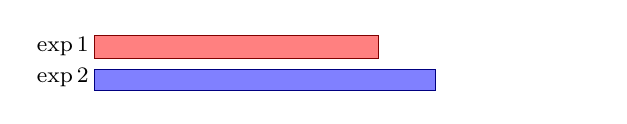
\begin{tikzpicture}[scale=0.4]
	\draw[color=white] (-2, -3) -- (16, -3);
	\node[font=\footnotesize] (e1) at (-1, -3.3) {$\exp{1}$};
	\node[font=\footnotesize] (e2) at (-1, -4.3) {$\exp{2}$};
	\filldraw[fill=red!50!white, draw=red!50!black] (0, -3.7) rectangle (9.02554, -2.9623);
	\filldraw[fill=blue!50!white, draw=blue!50!black] (0, -4.7) rectangle (10.8307, -4.04426);
\end{tikzpicture}
\end{center}
}

%\vspace{.05cm}

\uncover<3->{
\begin{center}
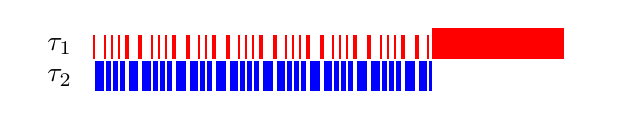
\begin{tikzpicture}[scale=0.4]
		\draw[color=white] (-2, -1) -- (16, -1);
% \draw[->] (-.2, -3.2) -- (15.2, -3.2) node[right] {time};
\node[] (t1) at (-1, -1.3) {$\tau_1$};
\node[] (t1) at (-1, -2.3) {$\tau_2$};
\fill[red] (0.0665893, -1.7) rectangle (0.130345, -0.929508);
\fill[blue] (0.130345, -2.7) rectangle (0.393197, -1.76557);
\fill[red] (0.393197, -1.7) rectangle (0.456953, -0.929508);
\fill[blue] (0.456953, -2.7) rectangle (0.614665, -1.76557);
\fill[red] (0.614665, -1.7) rectangle (0.67842, -0.929508);
\fill[blue] (0.67842, -2.7) rectangle (0.836132, -1.76557);
\fill[red] (0.836132, -1.7) rectangle (0.899887, -0.929508);
\fill[blue] (0.899887, -2.7) rectangle (1.0576, -1.76557);
\fill[red] (1.0576, -1.7) rectangle (1.18511, -0.929508);
\fill[blue] (1.18511, -2.7) rectangle (1.50053, -1.76557);
\fill[red] (1.50053, -1.7) rectangle (1.62804, -0.929508);
\fill[blue] (1.62804, -2.7) rectangle (1.8909, -1.76557);
\fill[red] (1.8909, -1.7) rectangle (1.95465, -0.929508);
\fill[blue] (1.95465, -2.7) rectangle (2.11236, -1.76557);
\fill[red] (2.11236, -1.7) rectangle (2.17612, -0.929508);
\fill[blue] (2.17612, -2.7) rectangle (2.33383, -1.76557);
\fill[red] (2.33383, -1.7) rectangle (2.39759, -0.929508);
\fill[blue] (2.39759, -2.7) rectangle (2.5553, -1.76557);
\fill[red] (2.5553, -1.7) rectangle (2.68281, -0.929508);
\fill[blue] (2.68281, -2.7) rectangle (2.99823, -1.76557);
\fill[red] (2.99823, -1.7) rectangle (3.12574, -0.929508);
\fill[blue] (3.12574, -2.7) rectangle (3.3886, -1.76557);
\fill[red] (3.3886, -1.7) rectangle (3.45235, -0.929508);
\fill[blue] (3.45235, -2.7) rectangle (3.61006, -1.76557);
\fill[red] (3.61006, -1.7) rectangle (3.67382, -0.929508);
\fill[blue] (3.67382, -2.7) rectangle (3.83153, -1.76557);
\fill[red] (3.83153, -1.7) rectangle (3.95904, -0.929508);
\fill[blue] (3.95904, -2.7) rectangle (4.27447, -1.76557);
\fill[red] (4.27447, -1.7) rectangle (4.40198, -0.929508);
\fill[blue] (4.40198, -2.7) rectangle (4.66483, -1.76557);
\fill[red] (4.66483, -1.7) rectangle (4.72858, -0.929508);
\fill[blue] (4.72858, -2.7) rectangle (4.8863, -1.76557);
\fill[red] (4.8863, -1.7) rectangle (4.95005, -0.929508);
\fill[blue] (4.95005, -2.7) rectangle (5.10776, -1.76557);
\fill[red] (5.10776, -1.7) rectangle (5.17152, -0.929508);
\fill[blue] (5.17152, -2.7) rectangle (5.32923, -1.76557);
\fill[red] (5.32923, -1.7) rectangle (5.45674, -0.929508);
\fill[blue] (5.45674, -2.7) rectangle (5.77216, -1.76557);
\fill[red] (5.77216, -1.7) rectangle (5.89968, -0.929508);
\fill[blue] (5.89968, -2.7) rectangle (6.16253, -1.76557);
\fill[red] (6.16253, -1.7) rectangle (6.22628, -0.929508);
\fill[blue] (6.22628, -2.7) rectangle (6.384, -1.76557);
\fill[red] (6.384, -1.7) rectangle (6.44775, -0.929508);
\fill[blue] (6.44775, -2.7) rectangle (6.60546, -1.76557);
\fill[red] (6.60546, -1.7) rectangle (6.66922, -0.929508);
\fill[blue] (6.66922, -2.7) rectangle (6.82693, -1.76557);
\fill[red] (6.82693, -1.7) rectangle (6.95444, -0.929508);
\fill[blue] (6.95444, -2.7) rectangle (7.26986, -1.76557);
\fill[red] (7.26986, -1.7) rectangle (7.39738, -0.929508);
\fill[blue] (7.39738, -2.7) rectangle (7.66023, -1.76557);
\fill[red] (7.66023, -1.7) rectangle (7.72398, -0.929508);
\fill[blue] (7.72398, -2.7) rectangle (7.8817, -1.76557);
\fill[red] (7.8817, -1.7) rectangle (7.94545, -0.929508);
\fill[blue] (7.94545, -2.7) rectangle (8.10316, -1.76557);
\fill[red] (8.10316, -1.7) rectangle (8.16692, -0.929508);
\fill[blue] (8.16692, -2.7) rectangle (8.32463, -1.76557);
\fill[red] (8.32463, -1.7) rectangle (8.45214, -0.929508);
\fill[blue] (8.45214, -2.7) rectangle (8.76756, -1.76557);
\fill[red] (8.76756, -1.7) rectangle (8.89508, -0.929508);
\fill[blue] (8.89508, -2.7) rectangle (9.15793, -1.76557);
\fill[red] (9.15793, -1.7) rectangle (9.22168, -0.929508);
\fill[blue] (9.22168, -2.7) rectangle (9.3794, -1.76557);
\fill[red] (9.3794, -1.7) rectangle (9.44315, -0.929508);
\fill[blue] (9.44315, -2.7) rectangle (9.60086, -1.76557);
\fill[red] (9.60086, -1.7) rectangle (9.66462, -0.929508);
\fill[blue] (9.66462, -2.7) rectangle (9.82233, -1.76557);
\fill[red] (9.82233, -1.7) rectangle (9.94984, -0.929508);
\fill[blue] (9.94984, -2.7) rectangle (10.2653, -1.76557);
\fill[red] (10.2653, -1.7) rectangle (10.3928, -0.929508);
\fill[blue] (10.3928, -2.7) rectangle (10.6556, -1.76557);
\fill[red] (10.6556, -1.7) rectangle (10.7194, -0.929508);
\fill[blue] (10.7194, -2.7) rectangle (10.8245, -1.76557);
\fill[red] (10.8245, -1.7) rectangle (15, -0.7);
\end{tikzpicture}
\end{center}
}



%\vspace{.05cm}

\uncover<4->{
\begin{center}
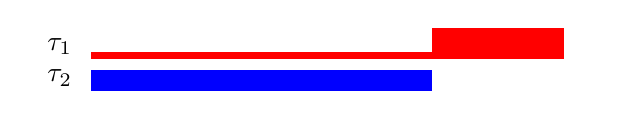
\begin{tikzpicture}[scale=0.4]
		\draw[color=white] (-2, -1) -- (16, -1);
% \draw[color=red, line width=2pt] (0,0) edge (9.02554,1.66572);
% \draw[color=red, line width=2pt] (9.02554,1.66572) edge (10.8307,1.515);
% \draw[color=red, line width=2pt] (10.8307,1.515) edge (15,0);
% \draw[color=blue, line width=2pt] (0,0) edge (9.02554,0);
% \draw[color=blue, line width=2pt] (9.02554,0) edge (10.8307,0);
% \draw[color=blue, line width=2pt] (10.8307,0) edge (15,0);
% \draw[color=black, line width=2pt] (0,0) edge (9.02554,2.90417);
% \draw[color=black, line width=2pt] (9.02554,2.90417) edge (10.8307,3.485);
% \draw[color=black, line width=2pt] (10.8307,3.485) edge (15,5);
\node[] (t1) at (-1, -1.3) {$\tau_1$};
\node[] (t1) at (-1, -2.3) {$\tau_2$};
% \draw[] (15.2, 5.2) node[right] {$m_m$};
% \draw[->] (-.2, -.2) -- (15.2, -.2) node[right] {time};
% \draw[->] (-.2, -.2) -- (-.2, 5.2) node[right] {memory};
% \draw[step=35.8423,very thin,color=gray] (0,0) grid (15, 5);
\fill[blue] (0, -2.7) rectangle (9.02554, -2.04426);
\fill[red] (0, -1.7) rectangle (9.02554, -1.4702);
\fill[blue] (9.02554, -2.7) rectangle (10.8307, -2.04426);
\fill[red] (9.02554, -1.7) rectangle (10.8307, -1.4702);
\fill[red] (10.8307, -1.7) rectangle (15, -0.7);
\end{tikzpicture}
\end{center}
}

\end{columns}


\end{frame}


\begin{frame}[fragile]
	\frametitle{Checking the Constraint}

\begin{center}
\begin{tikzpicture}[scale = 0.55]


%\draw (8.6353, -6.5) rectangle (15, -1);




\filldraw[fill=red!50!white, draw=red!50!black] (0, -4) rectangle (1.68224, -3.85714);
\filldraw[fill=green!50!white, draw=green!50!black] (0.841121, -6) rectangle (2.24299, -5.08571);
\filldraw[fill=red!50!white, draw=red!50!black] (4.48598, -4) rectangle (6.72897, -3.85714);
\filldraw[fill=blue!50!white, draw=blue!50!black] (5.04673, -5) rectangle (8.41121, -4.46429);
\filldraw[fill=green!50!white, draw=green!50!black] (7.85047, -6) rectangle (10.0935, -5.10714);
\filldraw[fill=red!50!white, draw=red!50!black] (7.57009, -4) rectangle (10.3738, -3.85714);
\filldraw[fill=blue!50!white, draw=blue!50!black] (9.25234, -5) rectangle (12.0561, -4.57143);
\filldraw[fill=green!50!white, draw=green!50!black] (11.215, -6) rectangle (12.6168, -5.08571);

\draw[->] (-.2, -.2) -- (15.2, -.2) node[right] {{\footnotesize time}};
\draw[->] (-.2, -.2) -- (-.2, 5.2) node[right] {{\footnotesize memory}};
\draw[step=46.9484,very thin,color=gray] (0,0) grid (15, 5);


\node[] (e1) at (-1, -4) {\scriptsize{$\exp{1}$}};
\node[] (e2) at (-1, -4.7) {\scriptsize{$\exp{2}$}};
\node[] (e3) at (-1, -5.6) {\scriptsize{$\exp{3}$}};


\uncover<1-> {


\node[] (t1) at (-1, -1.5) {\scriptsize{$\tau_1$}};

\draw[color=black, line width=1.5pt] (0,0) edge (0.841121,0.0704225);
\draw[color=green, line width=1.5pt] (0,0) edge (0.841121,0);
\draw[color=blue, line width=1.5pt] (0,0) edge (0.841121,0);
\draw[color=red, line width=1.5pt] (0,0) edge (0.841121,0);
\fill[red] (0, -1.7) rectangle (0.841121, -1.53607);
\only<1-3> \draw[dashed] (0.841121, -1) -- (0.841121, -6.5);

}
\uncover<2-> {


\node[] (t3) at (-1, -3.2) {\scriptsize{$\tau_3$}};

\draw[color=black, line width=1.5pt] (0.841121,0.0704225) edge (1.68224,0.413763);
\draw[color=green, line width=1.5pt] (0.841121,0) edge (1.68224,0.177786);
\draw[color=blue, line width=1.5pt] (0.841121,0) edge (1.68224,0);
\draw[color=red, line width=1.5pt] (0.841121,0) edge (1.68224,0);
\fill[red] (0.841121, -1.7) rectangle (1.68224, -1.53607);
\fill[green] (0.841121, -3.7) rectangle (1.68224, -3.06468);
\only<2-4> \draw[dashed] (1.68224, -1) -- (1.68224, -6.5);

}
\uncover<3-> {

\draw[color=black, line width=1.5pt] (1.68224,0.413763) edge (2.24299,0.634421);
\draw[color=green, line width=1.5pt] (1.68224,0.177786) edge (2.24299,0.257598);
\draw[color=blue, line width=1.5pt] (1.68224,0) edge (2.24299,0);
\draw[color=red, line width=1.5pt] (1.68224,0) edge (2.24299,0);
\fill[green] (1.68224, -3.7) rectangle (2.24299, -2.92951);
\only<3-5> \draw[dashed] (2.24299, -1) -- (2.24299, -6.5);

}
\uncover<4-> {

\draw[color=black, line width=1.5pt] (2.24299,0.634421) edge (2.89761,0.892019);
\draw[color=green, line width=1.5pt] (2.24299,0.257598) edge (2.89761,0);
\draw[color=blue, line width=1.5pt] (2.24299,0) edge (2.89761,0);
\draw[color=red, line width=1.5pt] (2.24299,0) edge (2.89761,0);
\fill[green] (2.24299, -3.7) rectangle (2.89761, -2.92951);
\only<4-6> \draw[dashed] (2.89761, -1) -- (2.89761, -6.5);

}
\uncover<5-> {

\draw[color=black, line width=1.5pt] (2.89761,0.892019) edge (4.48598,0.892019);
\draw[color=green, line width=1.5pt] (2.89761,0) edge (4.48598,0);
\draw[color=blue, line width=1.5pt] (2.89761,0) edge (4.48598,0);
\draw[color=red, line width=1.5pt] (2.89761,0) edge (4.48598,0);
\only<5-7> \draw[dashed] (4.48598, -1) -- (4.48598, -6.5);

}
\uncover<6-> {

\draw[color=black, line width=1.5pt] (4.48598,0.892019) edge (5.04673,0.938967);
\draw[color=green, line width=1.5pt] (4.48598,0) edge (5.04673,0);
\draw[color=blue, line width=1.5pt] (4.48598,0) edge (5.04673,0);
\draw[color=red, line width=1.5pt] (4.48598,0) edge (5.04673,0);
\fill[red] (4.48598, -1.7) rectangle (5.04673, -1.53607);
\only<6-8> \draw[dashed] (5.04673, -1) -- (5.04673, -6.5);

}
\uncover<7-> { 

\node[] (t2) at (-1, -2.4) {\scriptsize{$\tau_2$}};

\draw[color=black, line width=1.5pt] (5.04673,0.938967) edge (6.72897,1.5455);
\draw[color=green, line width=1.5pt] (5.04673,0) edge (6.72897,0);
\draw[color=blue, line width=1.5pt] (5.04673,0) edge (6.72897,0.0624813);
\draw[color=red, line width=1.5pt] (5.04673,0) edge (6.72897,0);
\fill[red] (5.04673, -1.7) rectangle (6.72897, -1.53607);
\fill[blue] (5.04673, -2.7) rectangle (6.72897, -2.15797);
\only<7-9> \draw[dashed] (6.72897, -1) -- (6.72897, -6.5);


}
\uncover<8-> {

\draw[color=black, line width=1.5pt] (6.72897,1.5455) edge (7.57009,1.84127);
\draw[color=green, line width=1.5pt] (6.72897,0) edge (7.57009,0);
\draw[color=blue, line width=1.5pt] (6.72897,0.0624813) edge (7.57009,0.0307911);
\draw[color=red, line width=1.5pt] (6.72897,0) edge (7.57009,0);
\fill[blue] (6.72897, -2.7) rectangle (7.57009, -2.01148);
\only<8-10> \draw[dashed] (7.57009, -1) -- (7.57009, -6.5);

}
\uncover<9-> {

\draw[color=black, line width=1.5pt] (7.57009,1.84127) edge (7.85047,1.94236);
\draw[color=green, line width=1.5pt] (7.57009,0) edge (7.85047,0);
\draw[color=blue, line width=1.5pt] (7.57009,0.0307911) edge (7.85047,0.0412047);
\draw[color=red, line width=1.5pt] (7.57009,0) edge (7.85047,0);
\fill[red] (7.57009, -1.7) rectangle (7.85047, -1.53607);
\fill[blue] (7.57009, -2.7) rectangle (7.85047, -2.15797);
\only<9-11> \draw[dashed] (7.85047, -1) -- (7.85047, -6.5);

}
\uncover<10-> {

\draw[color=black, line width=1.5pt] (7.85047,1.94236) edge (8.41121,2.14454);
\draw[color=green, line width=1.5pt] (7.85047,0) edge (8.41121,0.293427);
\draw[color=blue, line width=1.5pt] (7.85047,0.0412047) edge (8.41121,0.0620318);
\draw[color=red, line width=1.5pt] (7.85047,0) edge (8.41121,0);
\fill[red] (7.85047, -1.7) rectangle (8.41121, -1.53607);
\fill[blue] (7.85047, -2.7) rectangle (8.41121, -2.15797);
\only<10-12> \draw[dashed] (8.41121, -1) -- (8.41121, -6.5);

}
\uncover<11-> {

\draw[color=black, line width=1.5pt] (8.41121,2.14454) edge (8.6353,2.22533);
\draw[color=green, line width=1.5pt] (8.41121,0.293427) edge (8.6353,0.410685);
\draw[color=blue, line width=1.5pt] (8.41121,0.0620318) edge (8.6353,0);
\draw[color=red, line width=1.5pt] (8.41121,0) edge (8.6353,0);
\fill[red] (8.41121, -1.7) rectangle (8.6353, -1.53607);
\fill[blue] (8.41121, -2.7) rectangle (8.6353, -2.15797);
\only<11-13> \draw[dashed] (8.6353, -1) -- (8.6353, -6.5);

}
\uncover<12-> {

\draw[color=black, line width=1.5pt] (8.6353,2.22533) edge (9.25234,2.43154);
\draw[color=green, line width=1.5pt] (8.6353,0.410685) edge (9.25234,0.579024);
\draw[color=blue, line width=1.5pt] (8.6353,0) edge (9.25234,0);
\draw[color=red, line width=1.5pt] (8.6353,0) edge (9.25234,0);
\fill[red] (8.6353, -1.7) rectangle (9.25234, -1.53607);
\fill[green] (8.6353, -3.7) rectangle (9.25234, -3.20959);
\only<12-14> \draw[dashed] (9.25234, -1) -- (9.25234, -6.5);

}
\uncover<13-> {

\draw[color=black, line width=1.5pt] (9.25234,2.43154) edge (10.0935,2.73275);
\draw[color=green, line width=1.5pt] (9.25234,0.579024) edge (10.0935,0.999643);
\draw[color=blue, line width=1.5pt] (9.25234,0) edge (10.0935,0);
\draw[color=red, line width=1.5pt] (9.25234,0) edge (10.0935,0);
\fill[red] (9.25234, -1.7) rectangle (10.0935, -1.53607);
\fill[blue] (9.25234, -2.7) rectangle (10.0935, -2.2082);
\fill[green] (9.25234, -3.7) rectangle (10.0935, -3.65456);
\only<13-15> \draw[dashed] (10.0935, -1) -- (10.0935, -6.5);

}
\uncover<14-> {

\draw[color=black, line width=1.5pt] (10.0935,2.73275) edge (10.3738,2.83315);
\draw[color=green, line width=1.5pt] (10.0935,0.999643) edge (10.3738,0.993136);
\draw[color=blue, line width=1.5pt] (10.0935,0) edge (10.3738,0);
\draw[color=red, line width=1.5pt] (10.0935,0) edge (10.3738,0);
\fill[red] (10.0935, -1.7) rectangle (10.3738, -1.53607);
\fill[blue] (10.0935, -2.7) rectangle (10.3738, -2.2082);
\fill[green] (10.0935, -3.7) rectangle (10.3738, -3.65456);
\only<14-16> \draw[dashed] (10.3738, -1) -- (10.3738, -6.5);

}
\uncover<15-> {

\draw[color=black, line width=1.5pt] (10.3738,2.83315) edge (11.215,3.20121);
\draw[color=green, line width=1.5pt] (10.3738,0.993136) edge (11.215,0.836353);
\draw[color=blue, line width=1.5pt] (10.3738,0) edge (11.215,0);
\draw[color=red, line width=1.5pt] (10.3738,0) edge (11.215,0);
\fill[blue] (10.3738, -2.7) rectangle (11.215, -2.2082);
\fill[green] (10.3738, -3.7) rectangle (11.215, -3.33503);
\only<15-17> \draw[dashed] (11.215, -1) -- (11.215, -6.5);

}
\uncover<16-> {

\draw[color=black, line width=1.5pt] (11.215,3.20121) edge (12.0561,3.56926);
\draw[color=green, line width=1.5pt] (11.215,0.836353) edge (12.0561,1.13027);
\draw[color=blue, line width=1.5pt] (11.215,0) edge (12.0561,0);
\draw[color=red, line width=1.5pt] (11.215,0) edge (12.0561,0);
\fill[blue] (11.215, -2.7) rectangle (12.0561, -2.2082);
\fill[green] (11.215, -3.7) rectangle (12.0561, -3.33503);
\only<16-18> \draw[dashed] (12.0561, -1) -- (12.0561, -6.5);

}
\uncover<17-> {

\draw[color=black, line width=1.5pt] (12.0561,3.56926) edge (12.6168,3.85564);
\draw[color=black, line width=1.5pt] (12.6168,3.85564) edge (14.8575,5);
\draw[color=green, line width=1.5pt] (12.0561,1.13027) edge (12.6168,1.14436);
\draw[color=green, line width=1.5pt] (12.6168,1.14436) edge (14.8575,0);
\draw[color=blue, line width=1.5pt] (12.0561,0) edge (12.6168,0);
\draw[color=blue, line width=1.5pt] (12.6168,0) edge (14.8575,0);
\draw[color=red, line width=1.5pt] (12.0561,0) edge (12.6168,0);
\draw[color=red, line width=1.5pt] (12.6168,0) edge (14.8575,0);
\fill[green] (12.0561, -3.7) rectangle (14.8575, -2.7);

}

\end{tikzpicture}
\end{center}
% \uncover<5->{
% \begin{itemize}
% 	\item We can jump from \memph{"event"} to \memph{"event"}: \memph{$O(n \log n)$} worst case time complexity
% \end{itemize}
% }

\end{frame}



\begin{frame}[fragile]
  \frametitle{Sweep algorithm~\mycite{BeldiceanuCarlsson01}}
    
		\begin{itemize}
			\item The constraint can be checked in $\memph{O(n \log n)}$
			\pause \item Several experiments active simultaneously:
			\begin{itemize}
				\item Error is less than or equal to \memph{$1 + \frac{\tau^{max}}{\tau^{min}} \simeq 3$} blocks \\~
			\end{itemize}			
			\pause \item \memph{Faster and more accurate than the reservoir/transfer tasks model}
			
			\pause \item Bound adjustments? Two principles:
			\begin{itemize}
				\item Producing too much data too quickly can lead to data loss
				\item Filling up the mass memory while not in visibility can lead to data loss
			\end{itemize}
		\end{itemize}
	
\end{frame}


	\def\tsat{\overline{t}}


\begin{frame}[fragile]
\frametitle{Propagation: production/transfer rate}
\begin{myblock}{For a set of tasks}
\begin{itemize}
\item \memph{lower bound} on how much time the CDMS needs to transfer without data loss
\end{itemize}
\end{myblock}

\medskip

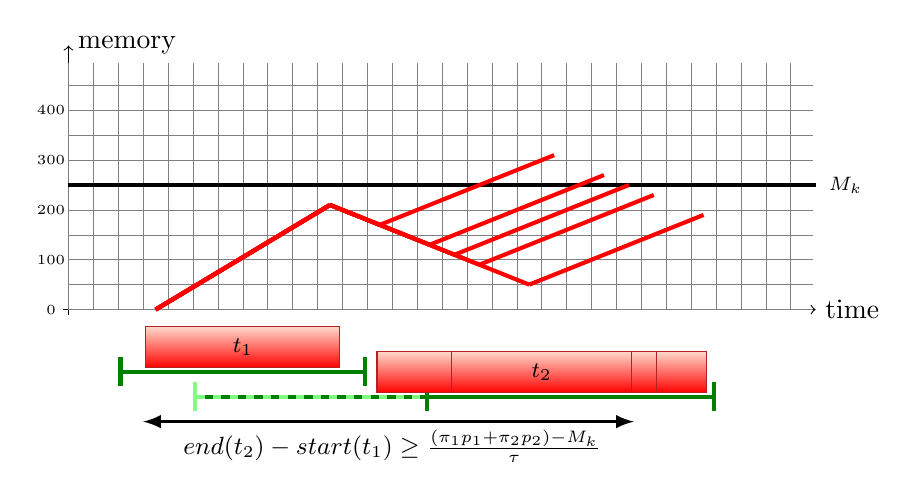
\begin{tikzpicture}[scale=0.9]
	
\tikzset{task/.style={draw=FireBrick,top color=OrangeRed!20, bottom color=Red, minimum height=15pt, shape=rectangle, font=\footnotesize}}
\tikzset{t1/.style={task, minimum width=70pt}}
\tikzset{t2/.style={task, minimum width=65pt}}
	
\node[t1] (t31) at (70pt,-15pt) {$t_1$};
\draw[|-|, ultra thick, green!50!black] (20pt,-25pt) -- (120pt,-25pt);

\uncover<1-4> {
\draw[|-|, ultra thick, green!50!black] (50pt,-35pt) -- (260pt,-35pt);
}

\uncover<5> {
\draw[|-, dashed, ultra thick, green!50] (50pt,-35pt) -- (143pt,-35pt);
\draw[|-|, ultra thick, green!50!black] (143pt,-35pt) -- (260pt,-35pt);
}

\draw[->] (-2pt,0pt) -- (300pt,0pt) node[right] {time};
\draw[->] (0pt,-2pt) -- (0pt,106pt) node[right] {memory};
\draw[step=10pt,very thin,color=gray] (0pt,0pt) grid (299pt,99pt);
\node[] (mark0) at (-7pt,0pt) {{\tiny 0}};
\node[] (mark20) at (-7pt,20pt) {{\tiny 100}};
\node[] (mark40) at (-7pt,40pt) {{\tiny 200}};
\node[] (mark60) at (-7pt,60pt) {{\tiny 300}};
\node[] (mark80) at (-7pt,80pt) {{\tiny 400}};

\draw[color=black, line width=1.5pt] (0pt,50pt) edge (300pt,50pt);
\node[] (mark0) at (312pt,50pt) {{\scriptsize $M_k$}};

\uncover<1>{
\node[t2] (t32) at (220pt,-25pt) {$t_2$};
\draw[color=red, line width=1.5pt] (35pt,0pt) edge (105pt,42pt);
\draw[color=red, line width=1.5pt] (105pt,42pt) edge (185pt,10pt);
\draw[color=red, line width=1.5pt] (185pt,10pt) edge (255pt,38pt);
}

\uncover<2>{
\node[t2] (t32) at (200pt,-25pt) {$t_2$};
\draw[color=red, line width=1.5pt] (35pt,0pt) edge (105pt,42pt);
\draw[color=red, line width=1.5pt] (105pt,42pt) edge (165pt,18pt);
\draw[color=red, line width=1.5pt] (165pt,18pt) edge (235pt,46pt);
}

\uncover<3>{
\node[t2] (t32) at (180pt,-25pt) {$t_2$};
\draw[color=red, line width=1.5pt] (35pt,0pt) edge (105pt,42pt);
\draw[color=red, line width=1.5pt] (105pt,42pt) edge (145pt,26pt);
\draw[color=red, line width=1.5pt] (145pt,26pt) edge (215pt,54pt);
}

\uncover<4>{
\node[t2] (t32) at (160pt,-25pt) {$t_2$};
\draw[color=red, line width=1.5pt] (35pt,0pt) edge (105pt,42pt);
\draw[color=red, line width=1.5pt] (105pt,42pt) edge (125pt,34pt);
\draw[color=red, line width=1.5pt] (125pt,34pt) edge (195pt,62pt);
}


\uncover<5>{
\node[t2] (t32) at (190pt,-25pt) {$t_2$};
\draw[color=red, line width=1.5pt] (35pt,0pt) edge (105pt,42pt);
\draw[color=red, line width=1.5pt] (105pt,42pt) edge (155pt,22pt);
\draw[color=red, line width=1.5pt] (155pt,22pt) edge (225pt,50pt);

\draw[latex-latex, very thick] (30pt,-45pt) -- (227pt,-45pt);
\node[] (mark0) at (130pt,-55pt) {{\small \memph{$end(t_2) - start(t_1) \geq \frac{(\pi_1 p_1 + \pi_2 p_2)-M_k}{\tau}$}}};
}


\end{tikzpicture}

\end{frame}


\begin{frame}
	\frametitle{Propagation: production/transfer rate}
	
	More generally, we consider a set of tasks \memph{$\Omega$} of a given experiment
	\begin{itemize}
		%\item Let \memph{$[a,b]=[\min_{t_{ki}\in \Omega}(\max(s_{ki})), \max_{t_{ki}\in \Omega}(\min(s_{ki}+p_{ki}))]$}
		\pause \item Let \memph{$[a,b]$} be a time interval \memph{necessarily} contained in \memph{$\Omega$}'s transfer period 
		\pause \item We can take into account the tasks of higher priority producing during \memph{$[a,b]$}
	\end{itemize}
	
\pause \begin{myblock}{Filtering rule}
\begin{itemize}
%\item Let \memph{$min(|t_{ki}\cap[a,b]|)$} be the minimal intersection between \memph{$t_{ki}$} and \memph{$[a,b]$}
\item 
Minimum amount of higher priority data to transfer on \memph{$[a,b]$} over transfer rate:
\begin{itemize}
	\item Lower bound on the time dedicated to higher priority experiment: \memph{$T_k(a,b)$}
\end{itemize}
% \begin{itemize}
% 	\item \memph{$\sum_{j=1}^{j<R(k)} \sum_{i=1}^n \min(|t_{P(j)i} \cap [a,b]|)*\pi_{P(j)i}$}
% \end{itemize}
% \pause
% \item Necessary duration:\\
% \hspace{1cm} \memph{$T_k(a,b)= \dfrac{\sum_{j=1}^{j<R(k)} \sum_{i=1}^n \min(|t_{P(j)i} \cap [a,b]|)*\pi_{P(j)i}}{\tau}$}
\pause 
\item Induced constraint:\\
\hspace{1cm} \memph{$Makespan(\Omega) \geq \frac{(\sum_{t_{ki}\in \Omega} \pi_i p_i)-M_k}{\tau} + T_k(a,b)$}
%\memph{$\max_{t_{ki} \in \Omega}(e_{ki}) - \min_{t_{ki} \in \Omega}(s_{ki}) \geq \frac{(\sum_{t_{ki}\in \Omega} \pi_i p_i)-M_k}{\tau} + T_k(a,b)$}

\end{itemize}
\end{myblock}

\end{frame}

	
	
\begin{frame}
  \frametitle{Propagation: visibility}
  
	
	\begin{itemize}
		\item When the mass memory is full, no more data is transferred to it
		\uncover<2->{\item Minimal usage and peak \memph{$m_0^{max}$}
%		\item Compute the date \memph{$\tsat$} at which the usage reaches its maximum \memph{$m_0^{\tsat}$}
		\uncover<3->{%\item Given an experiment with memory \memph{$M_k$}
		%\begin{itemize}
			\item If the production exceeds \memph{$M_k + M_0 - m_0^{max}$} in \memph{$[a, b]$} then data will be \memph{lost}
		%\end{itemize}
		\uncover<4->{
		\begin{itemize}
			\item \memph{Filtering: bound start time w.r.t. this quantity of data and production rate}
		\end{itemize}
		}
		}
		}
	\end{itemize}


\begin{center}
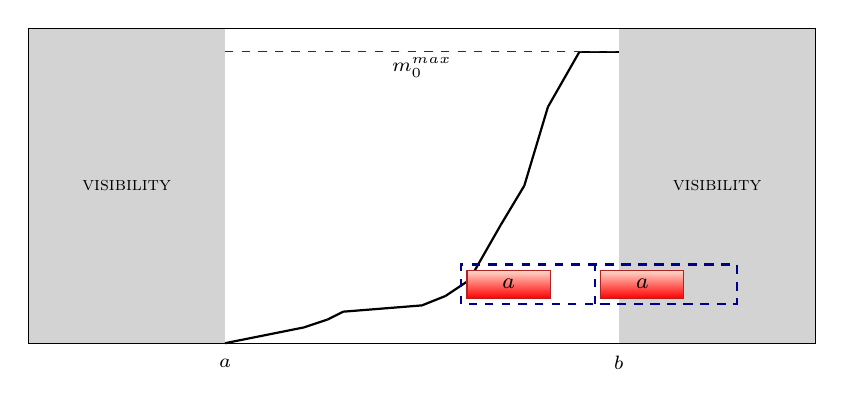
\begin{tikzpicture}
	
	\tikzset{task/.style={draw=FireBrick,top color=OrangeRed!20, bottom color=Red, minimum height=10pt, shape=rectangle, font=\footnotesize, minimum width=30pt}}
	
		 
		 \fill[color=LightGray] (0,0) rectangle (2.5,4);
		 \node[font=\scriptsize] at (1.25,2) {{\sc visibility}};
		 \fill[color=LightGray] (7.5,0) rectangle (10,4);
		 \node[font=\scriptsize] at (8.75,2) {{\sc visibility}};
		 \draw[color=black] (0,0) rectangle (10,4);
		 
		 \uncover<2-> {
		 \draw[thick] (2.5,0) -- (3.5,.2);
		 \draw[thick] (3.5,.2) -- (3.8,.3);
		 \draw[thick] (3.8,.3) -- (4,.4);
		 \draw[thick] (4,.4) -- (5,.48);
		 \draw[thick] (5,.48) -- (5.3,.6);
		 \draw[thick] (5.3,.6) -- (5.6,.8);
		 \draw[thick] (5.6,.8) -- (6,1.5);
		 \draw[thick] (6,1.5) -- (6.3,2);
		 \draw[thick] (6.3,2) -- (6.6,3);
		 \draw[thick] (6.6,3) -- (7,3.7);
		 \draw[thick] (7,3.7) -- (7.5,3.7);
		 
		 %\draw[dashed, color=red!60!black] (7,0) -- (7,4);
		 
		 \draw[dashed, color=red!60!black] (2.5,3.7) -- (7.5,3.7);
		 
%		 \node[font=\scriptsize] at (7, -.2) {$\tsat$};
		 \node[font=\scriptsize] at (2.5, -.25) {$a$};
		 \node[font=\scriptsize] at (7.5, -.25) {$b$};
		 \node[font=\scriptsize] at (5, 3.5) {\memph{$m_0^{max}$}};
		 }
		 
		 
		 \uncover<3> {
		 \draw[dashed, color=DarkBlue, thick] (5.5,.5) rectangle (9,1);
		 \node[task] at (6.1,.75) {$a$};
		 }
		 
		 \uncover<4> {
		 \draw[dashed, color=DarkBlue, thick] (7.2,.5) rectangle (9,1);
		 \node[task] at (7.8,.75) {$a$};
		 }
		 
				 
\end{tikzpicture}
\end{center}


\end{frame}

















% \input{src/sections/search.tex}

% \section{Single Machine Resource}
%
% \input{src/sections/disjunct.tex}

% \input{src/sections/unary.tex}


% \begin{frame}
%
% \begin{center}
%
% \input{theta.tex}
%
% \end{center}
%
% \end{frame}

% \section{Cumulative Resource}
%
% \section{Other Resources}


\begin{frame}[allowframebreaks]
	\frametitle{Bibliography}
	
	\AtNextBibliography{\tiny}
	\printbibliography

	
\end{frame}






\end{document}




